\documentclass[11pt]{article}
\usepackage[a4paper,margin=1in]{geometry}
\usepackage{amsmath,amssymb,amsthm,mathtools}
\usepackage[expansion=false]{microtype}
\usepackage{graphicx,booktabs,array}
\usepackage[font=small,labelfont=bf]{caption}
\usepackage[dvipsnames]{xcolor}
\usepackage{enumitem}
\usepackage[hidelinks,pdfusetitle]{hyperref}
\usepackage{xurl}
\usepackage[nameinlink,capitalise]{cleveref}
\setlist{nosep,leftmargin=1.5em}
\newtheorem{theorem}{Theorem}
\newtheorem{lemma}[theorem]{Lemma}
\newtheorem{proposition}[theorem]{Proposition}
\newtheorem{corollary}[theorem]{Corollary}
\theoremstyle{definition}\newtheorem{definition}[theorem]{Definition}
\theoremstyle{remark}\newtheorem{remark}[theorem]{Remark}
\newcommand{\R}{\mathbb R}\newcommand{\C}{\mathbb C}\newcommand{\N}{\mathbb N}
\newcommand{\dd}{\,\mathrm d}\newcommand{\e}{\mathrm e}
\renewcommand{\Re}{\operatorname{Re}}\renewcommand{\Im}{\operatorname{Im}}
\newcommand{\NH}{\mathrm{NH_3}}\newcommand{\HS}{\mathrm{H_2S}}\newcommand{\NHSH}{\mathrm{NH_4SH}}
\newcommand{\Hw}{\mathrm{H_2O}}\newcommand{\CH}{\mathrm{CH_4}}
\newcommand{\muH}{\,\mu\mathrm{Hz}}
\setlength{\parskip}{0.35em}
\AtBeginDocument{\sloppy}
\urlstyle{same}
\hypersetup{pdftitle={The Four Giants as Balanced Pairs: Throats, Hearts, the Gas Ladder and the Interstellar Visitors},pdfauthor={Abhijit Singh}}
\title{\textbf{The Four Giants as Balanced Pairs: Throats, Hearts, the Gas Ladder and the Interstellar Visitors}}
\author{Abhijit Singh}
\date{25 September 2026}
\begin{document}
\maketitle
\begin{abstract}
We show that each of the four giant planets is built of balanced pairs about a centre at four levels: its throats, its heart, its cloud decks and its place among the giants; the interstellar visitors and the planets of a pulsar meet the same structure. Every giant's Hill sphere opens through two throats, at $L_1$ and $L_2$, whose linear dynamics is the same for every planet, $\lambda^4-2\lambda^2-27=0$ ($\lambda^2-\omega^2=2$, $\lambda^2\omega^2=27$, vertical frequency $2$). The pair is unequal by $\mathcal A=\frac h3(1-\frac{h^2}{27}+O(h^3))$, $h=(\mu/3)^{1/3}$, and the full problem gives $0.99972$ to $1.00000$ of $h/3$ for the four giants and the planets of PSR~B1257+12. Near each throat the energy surface has the topology $S^2\times I$ of a spatial slice of the Einstein--Rosen bridge, in phase space; the flux through it is the action $2\pi\Delta E/\omega$ of its Lyapunov orbit, to $1.8\times10^{-6}$ at Jupiter's $L_1$, and every long temporary capture by Jupiter in the Ohtsuka catalogue entered and left through it. Jupiter and Saturn have dilute cores, and both carry tracking signals read as p-modes; the $n=1$ polytrope gives Jupiter's acoustic spacing to $4.5\%$ from mass and radius alone, and in polytropes matched to each planet's $J_2/q_\omega$ the $10^5$-bar level lies at $3569$ and $8786$ km, where the winds inferred from gravity end ($3000$ and $9000$ km). An equilibrium cloud-condensation model anchored at the $1$-bar temperatures gives $3,3,4,4$ cloud decks. The $\NHSH$ titration is an exact two-state pair, $x_{\NH}=k\e^{\varepsilon/2}$, $x_{\HS}=k\e^{-\varepsilon/2}$, whose survivor above the deck is $\mathrm{sign}(\mathrm N-\mathrm S)$. With deep $\mathrm{N/S}=4.73$, $3.16$, $0.195$ and $0.170$ this resolves why the ice giants show $\HS$ and not $\NH$ above their clouds: the model's saturated $\HS$ at the cloud tops is $0.26$--$1.8$ ppm on Uranus, which brackets the detected $0.4$--$0.8$ ppm, and $0.49$--$2.25$ ppm on Neptune, which overlaps the detected $1$--$3$ ppm.

The triangle of Jupiter--Saturn conjunctions turns one third of a turn in exactly one period of the great inequality, $883$ years. The four orbit planes precess in three live modes and one exact zero mode, the invariable plane. The triangular points are stable by the Gascheau--Routh criterion, with their spectrum on the imaginary axis in pairs of opposite Krein signature that leave it only by colliding, and Trojans are known at all four giants. The outermost moons of Jupiter, Saturn and Neptune reach $0.633$, $0.625$ and $0.654$ of the Hill radius and those of Uranus $0.407$; we predict retrograde moons $42$--$51$ million km from Uranus. The three interstellar objects share neither a direction nor a kinematic origin (largest pairwise velocity difference $75.5$ km/s). 3I/ATLAS touched Jupiter's Hill sphere, at $1.0011$ Hill radii ($1.0020$ by JPL), and was not the source of the Wow!\ signal: in 1977 it lay $8.3^\circ$ from the nearer beam centre, and a hydrogen-line transmitter on it would have been received $11.6$ channels from the Wow!. Its four OH lines are two pairs about one centre, $1612.2309+1720.5299=1665.4018+1667.3590$ MHz. PSR~B1257+12 holds a near-$3{:}2$ pair of planets whose angular momenta stand in the ratio $1.03\pm0.07$, and for its mass the horizon radius is exactly one third of the innermost stable orbit. The results rest on exact expansions and linear algebra of the restricted problem, on a thermodynamic model built from stated data, and on two-body propagation of the visitors against an ephemeris that reproduces JPL's approach of 3I/ATLAS to Jupiter to $3\times10^{-4}$ au.
\end{abstract}

\section{Introduction}\label{sec:intro}
The four giant planets have been measured closely in the last decade. Juno's radio tracking gives Jupiter's gravity field and Cassini's Grand Finale gave Saturn's \cite{Durante2020,Iess}; interior models fitted to these fields place a dilute core in Jupiter and a stably stratified core in Saturn \cite{Wahl,Militzer2024,MankovichFuller}; both tracking records carry signals read as normal modes \cite{Durante2022,Markham}; and hydrogen sulfide has been detected above the clouds of Uranus and Neptune \cite{Irwin2018,Irwin2019a}. Three interstellar objects have crossed the planetary region since 2017 \cite{Meech17,MPEC19,MPEC25}. The theory this paper applies to them is classical, and its main steps form a sequence (\cref{tab:prior}).

\begin{table}[!htb]\centering\small
\begin{tabular}{@{}l>{\raggedright\arraybackslash}p{4.6cm}>{\raggedright\arraybackslash}p{8.0cm}@{}}\toprule
year & authors & result\\\midrule
1843, 1874 & Gascheau; Routh \cite{Gascheau,Routh} & the equilateral configuration is linearly stable iff $27\sum_{i<j}m_im_j<(\sum_im_i)^2$\\
1968, 1969 & Conley; McGehee \cite{Conley,McGehee} & near a collinear point the planar energy surface is $S^2\times I$\\
1969, 1973 & Lewis; Weidenschilling, Lewis \cite{Lewis1969,WL73} & equilibrium cloud-condensation model of the giant planets\\
1990 & MacKay \cite{MacKay} & the flux over a saddle equals the action of its periodic orbit\\
1992, 2003 & Wolszczan, Frail; Konacki, Wolszczan \cite{WF92,KW03} & the planets of PSR~B1257+12; their masses and inclinations\\
1999 & Cabral, Schmidt \cite{Cabral} & stability of a ring of $N$ vortices with a centre\\
2005 & Atreya, Wong \cite{AtreyaWong} & coupled clouds and chemistry; the NH$_4$SH equilibrium constant\\
2018, 2019 & Irwin et al.\ \cite{Irwin2018,Irwin2019a} & H$_2$S above the clouds of Uranus and Neptune\\
2021 & Molter et al.\ \cite{Molter2021} & deep $\mathrm{N/S}=0.20$ in Uranus\\
2021 & Mankovich, Fuller \cite{MankovichFuller} & a diffuse, stably stratified core in Saturn from ring seismology\\\bottomrule
\end{tabular}
\caption{Prior results this paper builds on.}\label{tab:prior}
\end{table}

\paragraph{Companion papers.} The restricted problem treated here is the three-body problem of the physics companion \cite{SPhys} with one vanishing mass: its Lagrange triangle, which grows at exactly $\omega/\sqrt2$ for equal masses, is here the pair of triangular points stable by the Gascheau--Routh criterion \cite{Gascheau,Routh}, and its figure-eight holds the triad $(-s,0,s)$ that the throats hold as a pair about a centre. The chemistry companion \cite{SChem} derives the two-state law of a metal-oxide gas sensor, $p=1/(1+\e^{\varepsilon})$, and measures the sensor ladder of an urban air record; the $\NHSH$ deck of \cref{sec:ladder} obeys the same law, and \cref{sec:pairlaw} states exactly what is shared. The mathematics and quantum companions \cite{SMath,SQuant} show that the zeros of $\xi$ lie on the critical line exactly when each is its own mirror image, and that a positive merge of spins keeps every Lee--Yang zero on its circle while a negative coupling lets zeros leave in mirrored pairs; the spectrum at the triangular points (\cref{prop:krein}) carries the same Klein four-group as these zeros, with the imaginary axis as its fixed line, and its eigenvalues leave that line only where two pairs of opposite Krein signature meet. The survivor $\mathrm{sign}(\mathrm N-\mathrm S)\in\{-1,0,1\}$ of the titration is a balanced-ternary digit \cite{SAlg}. The synthesis paper \cite{SZero} collects these readings of a zero.

\subsection{Main results}\label{sec:main}
\begin{enumerate}[label=\textbf{\arabic*.},leftmargin=1.8em]
\item \emph{Two throats about one centre} (\cref{sec:hill,sec:full}). The collinear points of Hill's problem have the characteristic polynomial $\lambda^4-2\lambda^2-27=0$ for every planet, so $\lambda_H^2-\omega_H^2=2$ and $\lambda_H^2\omega_H^2=27$, with vertical frequency $2$. The two throats are unequal by $\mathcal A=\frac h3\bigl(1-\frac{h^2}{27}+O(h^3)\bigr)$, $h=(\mu/3)^{1/3}$ (\cref{prop:asym}). In the full restricted problem $\mathcal A/(h/3)$ is $0.99972$ for Jupiter and within $10^{-5}$ of $1$ for the planets of PSR~B1257+12, and the largest relative departure of a linear rate from its Hill value is $0.96h$ to $1.01h$ (\cref{tab:throats}).
\item \emph{The throat in phase space} (\cref{sec:topology}). Near each throat the planar energy surface is $S^2\times I$, the topology of a spatial slice of the Einstein--Rosen bridge. The flux through the throat is the action $2\pi\Delta E/\omega$ of its Lyapunov orbit, which the computed orbits at Jupiter's $L_1$ approach monotonically, to $1.000002$ times it at amplitude $0.0018\,r_H$. The quantum transmission through the saddle is the two-state law $T=1/(1+\e^{-2\pi\Delta E/\hbar\lambda})$, equal to $\frac12$ at the saddle energy. Every long temporary capture of a comet by Jupiter in the Ohtsuka catalogue entered and left through the $L_1$ or $L_2$ region.
\item \emph{The hearts} (\cref{sec:hearts}). The $n=1$ polytrope has Love number $k_2=15/\pi^2-1$ and $J_2/q_\omega=0.17327$ (\cref{prop:love}), and all four giants lie below it, Saturn lowest at $0.10303$. The same polytrope gives Jupiter's acoustic spacing as $162.3\muH$, $4.5\%$ above the measured $155.3\pm2.2\muH$, from mass and radius alone. Jupiter and Saturn hold their heavy elements in dilute cores and both carry tracking signals read as p-modes. In polytropes matched to each planet's $J_2/q_\omega$ the $10^5$-bar level lies at $3569$ and $8786$ km, where the winds inferred from gravity end ($3000$ and $9000$ km), and we predict Saturn's acoustic spacing at $112$--$117\muH$. A ring of $N$ equal vortices with a centre is spectrally stable exactly on the intervals of Cabral and Schmidt's theorem, and three equal vortices with an equal fourth at the centre sit exactly on the edge.
\item \emph{The gas ladder} (\cref{sec:ladder}). An equilibrium cloud-condensation model built from stated thermodynamic data and anchored at the $1$-bar temperatures reproduces published cloud bases (NH$_3$ ice on Jupiter within $1.5$--$2.0\%$ of Atreya and Wong) and gives $3,3,4,4$ cloud decks (\cref{tab:decks}). The $\NHSH$ titration is an exact two-state pair (\cref{thm:titration}): where the solid coexists with the gas, $x_{\NH}=k\e^{\varepsilon/2}$ and $x_{\HS}=k\e^{-\varepsilon/2}$ with $k^2=K(T)/P^2$, the odd part $\mathrm N-\mathrm S$ is conserved, and the survivor above the deck is $\mathrm{sign}(\mathrm N-\mathrm S)$. The deep ratios $\mathrm{N/S}=4.73$, $3.16$, $0.195$ and $0.170$ of Jupiter, Saturn, Uranus and Neptune therefore leave NH$_3$ above the gas giants and H$_2$S above the ice giants. This resolves why the ice giants show H$_2$S and not NH$_3$ above their clouds: the model's saturated H$_2$S at the cloud tops is $0.26$--$1.8$ ppm on Uranus, which brackets the detected $0.4$--$0.8$ ppm, and $0.49$--$2.25$ ppm on Neptune, which overlaps the detected $1$--$3$ ppm. The deck and a metal-oxide gas sensor obey one two-state law (\cref{sec:pairlaw}).
\item \emph{The trigon} (\cref{prop:trigon}). Each corner of the triangle of Jupiter--Saturn conjunctions turns at $\frac13(5n_S-2n_J)$, so the trigon advances one third of a turn in exactly one period of the great inequality, $883$ years.
\item \emph{The zero mode} (\cref{prop:zeromode}). The Laplace--Lagrange inclination matrix of the four giants has the exact eigenvalue $0$, whose invariant plane is the invariable plane, and three live modes, $-25.5183$, $-2.9276$ and $-0.6698$ arcsec/yr.
\item \emph{Gascheau--Routh and Krein} (\cref{sec:triangle,sec:chain,sec:reach}). The triangular points are stable exactly for $\mu<\mu_G=0.0385209$, and a stable triangle needs a dominant centre, $m_1>0.9614791\,M$. Below $\mu_G$ the spectrum at $L_4$ lies on the imaginary axis in two pairs of opposite Krein signature, which leave the axis only by colliding at $\omega=1/\sqrt2$ (\cref{prop:krein}). All four giants satisfy the criterion, and Trojans are known at all four. Every orbit tangent to two neighbouring giants lies below both throat energies (\cref{prop:tisserand}). The outermost moons of Jupiter, Saturn and Neptune reach $0.633$, $0.625$ and $0.654$ of the Hill radius and those of Uranus $0.407$, and we predict undiscovered retrograde moons of Uranus $42$--$51$ million km from the planet.
\item \emph{The visitors} (\cref{sec:visitors}). The three interstellar objects share neither a direction nor a kinematic origin: no statistic of their incoming directions departs from isotropic or kinematic populations (smallest $p=0.27$), and their largest pairwise velocity difference, $75.5$ km/s, lies at the median, $75.4$ km/s, of random triples from the kinematic population. 3I/ATLAS touched Jupiter's Hill sphere on 16 March 2026, at $1.0011$ Hill radii ($1.0020$ by JPL). 3I/ATLAS was not the source of the Wow!\ signal: in 1977 it lay $8.3^\circ$ from the nearer beam centre, and a hydrogen-line transmitter on it would have been received $11.6$ channels from the Wow!. Its four OH lines are two pairs about one centre, $1612.2309+1720.5299=1665.4018+1667.3590$ MHz, and its OH lines changed from absorption to emission between heliocentric radial velocities $+13.37$ and $+20.93$ km/s, where the inversion crosses zero.
\item \emph{PSR B1257+12} (\cref{sec:pulsar}). The pulsar's planets B and C carry the giants' two throats, unequal by $h/3$ to $10^{-5}$, lie $1.60\%$ inside the $3{:}2$ resonance and carry angular momenta in the ratio $L_C/L_B=1.03\pm0.07$. For a mass $M$ the horizon, the photon sphere and the innermost stable circular orbit stand at $2$, $3$ and $6$ in units of $GM/c^2$, so the horizon radius is exactly one third of the innermost stable orbit.
\end{enumerate}

\subsection{Outline of the method}\label{sec:outline}
The throat results are exact expansions of the collinear equilibrium conditions and linear algebra of the restricted problem; the full-problem values come from root finding, and the flux from Lyapunov orbits computed by differential correction. The hearts use the exact Love number of the $n=1$ polytrope, first-order Clairaut theory on Lane--Emden profiles and the analytic Jacobian of the $N+1$ vortex problem. The gas ladder integrates the dry adiabat of normal hydrogen, with heat capacities from the rotational levels of H$_2$, by the fourth-order Runge--Kutta method in $\ln P$ from the NSSDC $1$-bar temperatures, and locates each deck base as the balance point of its saturation ratio by root bracketing; the titration theorem follows from mass action and one-for-one consumption. The results on the set follow from the mean motions, the Laplace--Lagrange matrix and the linearisation at $L_4$, with Krein signatures computed from the quadratic Hamiltonian. The visitors are propagated on their two-body hyperbolae against planetary positions from the orbital elements and periodic terms of Schlyter's method \cite{Schlyter}, rotated to the J2000 ecliptic; this ephemeris reproduces JPL's closest approach of 3I/ATLAS to Jupiter, $0.358330$ au at 12:22 UT on 16 March 2026, as $0.358011$ au at 11:33 UT (\cref{sec:contact}). Their directions and velocities are compared with isotropic and kinematic populations by Monte Carlo sampling ($10^6$ draws).

\subsection{Organisation and notation}\label{sec:org}
\Cref{sec:giants} collects the planetary data. \Cref{sec:throats} treats the throats, \cref{sec:hearts} the hearts, \cref{sec:ladder} the gas ladder, \cref{sec:set} the giants as a set, \cref{sec:visitors} the visitors and \cref{sec:pulsar} the planets of PSR~B1257+12; \cref{sec:discussion} sets the structure out level by level. Every computed number is obtained from the stated closed forms, by root finding, by numerical linear algebra, by numerical integration of the stated equations, or by Monte Carlo sampling of the stated populations, by the method given where the number appears; arithmetic is IEEE double precision. Frequencies in hertz are written $\nu$; dimensionless frequencies in a rotating frame, in units of the mean motion, are written $\omega$. $\mathrm N$ and $\mathrm S$ are the deep mole fractions of NH$_3$ and H$_2$S, and $r_H$ is the Hill radius.

\section{The four giants}\label{sec:giants}
\Cref{tab:giants} collects the data used throughout. The rotation parameter is $q_\omega=\omega_\mathrm{rot}^2R^3/GM$ at the reference radius $R$ of each gravity field, and $J_2/q_\omega$ measures how strongly mass gathers towards the centre (\cref{sec:love}). Hubble's auroral record gives Uranus's day as $17.247864$ h, $28$ s longer than Voyager's value \cite{Lamy}; we use it. Uranus's obliquity is $97.77^\circ$ and Neptune's $28.32^\circ$; their magnetic dipoles are tilted by $58.6^\circ$ and $46.9^\circ$ and offset by $0.352$ and $0.485$ planetary radii \cite{NSSDCU,NSSDCN}. By the counts of April and June 2026, Jupiter has $115$ known moons and Saturn $293$ with confirmed orbits; Uranus has $29$, including S/2025~U~1, and Neptune $16$ \cite{WikiMoons}.

\begin{table}[!htb]\centering\small\setlength{\tabcolsep}{4pt}
\begin{tabular}{@{}lcccccccc@{}}\toprule
 & $GM$ & $a$ & $R$ & $J_2$ & rotation & $q_\omega$ & $J_2/q_\omega$ & $I/MR^2$\\
 & ($10^6$ km$^3$s$^{-2}$) & ($10^6$ km) & (km) & ($10^{-6}$) & & & & \\\midrule
Jupiter & $126.687$ & $778.479$ & $71492$ & $14696.5735$ & $9.9250$ h & $0.08919$ & $0.16477$ & $0.2582$\\
Saturn & $37.931$ & $1432.041$ & $60330$ & $16290.573$ & $10^\mathrm{h}33^\mathrm{m}38^\mathrm{s}$ & $0.15812$ & $0.10303$ & $0.2189$\\
Uranus & $5.7940$ & $2867.043$ & $25559$ & $3343.43$ & $17.247864$ h & $0.02951$ & $0.11331$ & $0.2259$\\
Neptune & $6.8351$ & $4514.953$ & $24764$ & $3411$ & $16.11$ h & $0.02608$ & $0.13080$ & $0.2374$\\\bottomrule
\end{tabular}
\caption{The four giants. $GM$, $a$ and the rotation of Jupiter and Neptune from the NSSDC fact sheets \cite{NSSDCJ,NSSDCS,NSSDCU,NSSDCN}; $J_2$ of Jupiter from Juno \cite{Durante2020} and of Saturn from Cassini \cite{Iess}, at the reference radii shown; $J_2$ of Uranus and Neptune from NSSDC at the equatorial radius; Saturn's rotation from ring seismology \cite{Mankovich2019}; Uranus's from \cite{Lamy}. The $n=1$ polytrope has $J_2/q_\omega=0.17327$ (\cref{prop:love}); smaller values mean more mass towards the centre. Last column: the first-order Radau--Darwin moment of inertia (\cref{sec:love}).}\label{tab:giants}
\end{table}

\section{Two throats about one centre}\label{sec:throats}
\subsection{Hill's problem and the universal quartic}\label{sec:hill}
In the frame turning with a planet of mass fraction $\mu=m/(M+m)$ about a star of mass $M$, with the separation, the mean motion $n$ and $G(M+m)$ set to one, a test body keeps the Jacobi constant
\[
C=2U-v^2,\qquad U=\tfrac12(x^2+y^2)+\frac{1-\mu}{r_1}+\frac{\mu}{r_2},
\]
where $r_1,r_2$ are its distances from the star and the planet \cite{MD}. Near the planet, lengths scale with $\mu^{1/3}$; in these units (Hill's units) and in the limit $\mu\to0$ the equations of motion become Hill's equations,
\[
\ddot x-2\dot y=3x-\frac{x}{r^3},\qquad \ddot y+2\dot x=-\frac{y}{r^3},\qquad \ddot z=-z-\frac{z}{r^3},
\]
which are the same for every planet. They derive from the effective potential $U_H=\frac32x^2-\frac12z^2+1/r$. On the $x$-axis, $\partial_xU_H=3x-x/r^3=0$ gives the two collinear points $x=\pm3^{-1/3}=\pm0.693361$, where $r^3=\frac13$. There $\partial^2_{xx}(1/r)=2/r^3$ and $\partial^2_{yy}(1/r)=\partial^2_{zz}(1/r)=-1/r^3$, so
\[
U_{xx}=3+\tfrac2{r^3}=9,\qquad U_{yy}=-\tfrac1{r^3}=-3,\qquad U_{zz}=-1-\tfrac1{r^3}=-4 .
\]
The linearised planar equations $\ddot x-2\dot y=U_{xx}x$, $\ddot y+2\dot x=U_{yy}y$ have solutions $\e^{\lambda t}$ when $\det\begin{pmatrix}\lambda^2-U_{xx}&-2\lambda\\2\lambda&\lambda^2-U_{yy}\end{pmatrix}=0$, that is
\begin{equation}\label{eq:quartic}
\lambda^4+(4-U_{xx}-U_{yy})\lambda^2+U_{xx}U_{yy}=\lambda^4-2\lambda^2-27=0 .
\end{equation}
Hence $\lambda^2=1\pm2\sqrt7$: a real pair $\pm\lambda_H$, $\lambda_H=\sqrt{1+2\sqrt7}=2.508287$, and an imaginary pair $\pm i\omega_H$, $\omega_H=\sqrt{2\sqrt7-1}=2.071594$; the vertical motion adds $\pm2i$. The two roots in $\lambda^2$ have sum $2$ and product $-27$, so
\[
\lambda_H^2-\omega_H^2=2,\qquad \lambda_H^2\,\omega_H^2=27=3^3 .
\]
The numbers $2$ and $3^3$ fix every planet's throat. Departures from the saddle grow by a factor $\e$ in $1/\lambda_H$ of the time unit $1/n$, that is in $P_\mathrm{orb}/(2\pi\lambda_H)=P_\mathrm{orb}/15.7600$ of the planet's orbital period. The eigenvalues of the Jacobian of Hill's equations agree with these roots to $4.4\times10^{-16}$.

\subsection{The full problem: every giant carries the same pair}\label{sec:full}
In the full restricted problem we located $L_1$ and $L_2$ by root finding and computed the eigenvalues of the linearisation for the four giants and for the three planets of PSR~B1257+12 (\cref{sec:pulsar}). \Cref{tab:throats} lists them. For every body the largest departure of a rate from its Hill value lies between $0.96h$ and $1.01h$, with $h=(\mu/3)^{1/3}$. In the full problem the $e$-folding time at Jupiter's $L_1$ is $257.26$ days.

\begin{table}[!htb]\centering\footnotesize\setlength{\tabcolsep}{4pt}
\begin{tabular}{lccccccc}\toprule
 & $\mu$ & $r_H$ (Mkm) & $L_1$, $L_2$ (Mkm) & $\mathcal A/(h/3)$ & $\lambda$ at $L_1$, $L_2$ & $C(L_1)$ & libr.\ (yr) \\\midrule
Jupiter & $9.537\times10^{-4}$ & $53.130$ & $51.906$, $54.322$ & $0.99972$ & $2.681$, $2.352$ & $3.038756$ & $147.4$\\
Saturn & $2.857\times10^{-4}$ & $65.399$ & $64.392$, $66.383$ & $0.99989$ & $2.622$, $2.402$ & $3.017821$ & $670.2$\\
Uranus & $4.366\times10^{-5}$ & $69.997$ & $69.423$, $70.562$ & $0.99997$ & $2.568$, $2.451$ & $3.005219$ & $4893$\\
Neptune & $5.150\times10^{-5}$ & $116.471$ & $115.462$, $117.465$ & $0.99997$ & $2.572$, $2.447$ & $3.005818$ & $8837$\\
PSR B & $9.225\times10^{-6}$ & $0.7821$ & $0.7783$, $0.7858$ & $0.99999$ & $2.544$, $2.474$ & $3.001872$ & $23.09$\\
PSR C & $8.367\times10^{-6}$ & $0.9814$ & $0.9767$, $0.9859$ & $0.99999$ & $2.543$, $2.475$ & $3.001755$ & $35.78$\\\bottomrule
\end{tabular}
\caption{The throats in the full restricted problem. $\mu=m/(M+m)$ and $r_H=a(\mu/3)^{1/3}$, from the NSSDC values of \cref{tab:giants}; the pulsar planets from the timing solution of \cite{KW03} with a $1.4\,M_\odot$ pulsar (\cref{sec:pulsar}). \Cref{sec:reach} uses $r_H=a(m/3M_\odot)^{1/3}$, $0.03\%$ larger at Jupiter. $\mathcal A=(\gamma_2-\gamma_1)/(\gamma_2+\gamma_1)$, with $\gamma_{1,2}$ the distances of $L_{1,2}$ from the planet; $\lambda$ in units of the mean motion (Hill value $2.5083$); $C(L_1)$ the Jacobi constant at $L_1$; last column, the Trojan libration period at $L_4$ (\cref{sec:triangle}).}\label{tab:throats}
\end{table}

\begin{proposition}[the pair is unequal by a third]\label{prop:asym}
Let $\gamma_1$, $\gamma_2$ be the distances of $L_1$ and $L_2$ from the planet and $h=(\mu/3)^{1/3}$. Then
\[
\gamma_1=h-\tfrac{h^2}3-\tfrac{h^3}9+\tfrac{58}{81}h^4+O(h^5),\qquad \gamma_2=h+\tfrac{h^2}3-\tfrac{h^3}9+\tfrac{50}{81}h^4+O(h^5),
\]
and
\[
\mathcal A=\frac{\gamma_2-\gamma_1}{\gamma_2+\gamma_1}=\frac h3\Bigl(1-\frac{h^2}{27}+O(h^3)\Bigr).
\]
\end{proposition}
\begin{proof}
Place the star at $x=-\mu$ and the planet at $x=1-\mu$. At $L_1$, $x=1-\mu-\gamma$, the centrifugal term, the star's pull and the planet's pull balance: $1-\mu-\gamma-(1-\mu)(1-\gamma)^{-2}+\mu\gamma^{-2}=0$. Expanding $(1-\gamma)^{-2}=1+2\gamma+3\gamma^2+4\gamma^3+5\gamma^4+\dots$, the constant terms cancel and $\mu=\gamma^3+(1-\mu)(2\gamma^3+3\gamma^4+4\gamma^5+5\gamma^6+\dots)$. Since $\mu=3\gamma^3(1+O(\gamma))$, the term $-2\mu\gamma^3$ equals $-6\gamma^6+O(\gamma^7)$, and
\[
\tfrac\mu3=\gamma^3\bigl(1+\gamma+\tfrac43\gamma^2-\tfrac13\gamma^3+O(\gamma^4)\bigr).
\]
At $L_2$, $x=1-\mu+\gamma$, the balance is $1-\mu+\gamma-(1-\mu)(1+\gamma)^{-2}-\mu\gamma^{-2}=0$, and the same steps with $(1+\gamma)^{-2}=1-2\gamma+3\gamma^2-4\gamma^3+5\gamma^4-\dots$ give $\frac\mu3=\gamma^3(1-\gamma+\frac43\gamma^2-\frac{11}3\gamma^3+O(\gamma^4))$. With $\mu/3=h^3$ and $(1+u)^{1/3}=1+\frac u3-\frac{u^2}9+\frac{5u^3}{81}+O(u^4)$,
\[
h=\gamma\bigl(1+\tfrac\gamma3+\tfrac{\gamma^2}3-\tfrac{28}{81}\gamma^3\bigr)\ \text{at }L_1,\qquad h=\gamma\bigl(1-\tfrac\gamma3+\tfrac{\gamma^2}3-\tfrac{80}{81}\gamma^3\bigr)\ \text{at }L_2,
\]
up to $O(\gamma^5)$. Substituting $\gamma=h+c_2h^2+c_3h^3+c_4h^4$ and equating powers of $h$ gives $c_2=\mp\frac13$, $c_3=-\frac19$ and $c_4=\frac{58}{81}$, $\frac{50}{81}$ at $L_1$, $L_2$, which are the stated expansions. Hence $\gamma_2-\gamma_1=\frac23h^2-\frac8{81}h^4+O(h^5)$ and $\gamma_2+\gamma_1=2h-\frac29h^3+O(h^4)$, so
\[
\mathcal A=\frac h3\cdot\frac{1-\frac4{27}h^2+O(h^3)}{1-\frac19h^2+O(h^3)}=\frac h3\Bigl(1-\frac4{27}h^2+\frac19h^2+O(h^3)\Bigr)=\frac h3\Bigl(1-\frac{h^2}{27}+O(h^3)\Bigr).
\]
\end{proof}
The throats are a pair about the planet, $L_1$ on the star side and $L_2$ outside, unequal by exactly one third of $h$ at first order. The computed $\mathcal A/(h/3)$ is $0.99972$ for Jupiter and within $10^{-5}$ of $1$ for the pulsar planets (\cref{tab:throats}); $|\mathcal A/(h/3)-1|$ never exceeds $0.0041h$. Solving the equilibrium conditions in $50$-digit arithmetic for $\mu=10^{-9}$ and $10^{-6}$, $\gamma_{1,2}/h$ agree with the expansions of \cref{prop:asym} to $0.2h^4$, and $(\mathcal A/(h/3)-1)/h^2=-0.037268$ and $-0.039351$, which are $-\frac1{27}-\frac h3$ to $3\times10^{-8}$ and $3\times10^{-6}$: the next coefficient is $-\frac13$. For Jupiter, $1-\frac{h^2}{27}-\frac{h^3}3=0.99972$, the value in \cref{tab:throats}.

\subsection{The throat in phase space}\label{sec:topology}
For Jacobi constants between $C(L_2)$ and $C(L_1)$ only the $L_1$ throat is open; between $C(L_3)$ and $C(L_2)$ both are (for Jupiter, $3.000954<C<3.037484$). The zero-velocity surface $2U=C$ is closed everywhere else, so a body can enter or leave the planet's realm only through the throats (\cref{fig:throats}a). Conley and McGehee showed that near each throat the planar energy surface is a sphere times an interval, $S^2\times I$ \cite{Conley,McGehee}. In the spatial problem it is $S^4\times I$; it contains an invariant $3$-sphere, whose stable and unstable manifolds are tubes $S^3\times\R$ that separate transit from non-transit orbits \cite{KLMR,Gomez}. A spatial slice through the Schwarzschild wormhole of Einstein and Rosen \cite{ER} is $S^2\times\R$ \cite{MTW}. Near each throat, therefore, the energy surface has the topology $S^2\times I$ of an Einstein--Rosen slice, in phase space, and the tubes play the part of the bridge: they carry every orbit that passes from one realm to the other. A wormhole in spacetime would also lens the light of stars behind it and pull on nearby bodies through its mass; the appearance of such a wormhole near Saturn was computed from general relativity for the film \emph{Interstellar} \cite{JamesWormhole}. Cassini's radio ranging to Saturn is precise enough to constrain where an unseen ninth planet could lie far beyond it \cite{Fienga}, and the one signal in its tracking that the gravity field did not absorb is read as Saturn's own oscillations (\cref{sec:saturnheart}).

\paragraph{The flux through the throat, and its quantum form.} In planar normal coordinates near the throat, $H=\lambda q_1p_1+\frac\omega2(q_2^2+p_2^2)$. At energy $\Delta E$ above the saddle the periodic (Lyapunov) orbit is the circle $\frac\omega2(q_2^2+p_2^2)=\Delta E$, $q_1=p_1=0$, of radius $\sqrt{2\Delta E/\omega}$, and its action is the enclosed area,
\[
\oint p\dd q=\pi\cdot\frac{2\Delta E}{\omega}=\frac{2\pi\Delta E}{\omega}.
\]
MacKay proved that the flux of orbits across the dividing surface through a saddle equals the action of this periodic orbit \cite{MacKay}. For Lyapunov orbits computed by differential correction at Jupiter's $L_1$, the ratio of the action to $2\pi\Delta E/\omega$ falls monotonically from $1.001274$ (amplitude $0.044\,r_H$) to $1.000002$ ($0.0018\,r_H$), the orbits closing to better than $1.1\times10^{-12}$. In chemistry this orbit is a reaction's transition state: Porter and Cvitanovi\'c call the orbits about $L_1$ and $L_2$ ``the transition states \ldots\ controlling transport through the bottleneck'' \cite{PorterCv}, and Jaff\'e and co-workers computed asteroid escape rates from them with the statistical rate theory of molecules \cite{Jaffe}. Quantum mechanically, a mode crossing such a saddle with energy $\Delta E$ above it is transmitted with probability
\[
T(\Delta E)=\frac1{1+\e^{-2\pi\Delta E/\hbar\lambda}}
\]
(the parabolic barrier of \cite[\S50]{LL}), and the transverse channels open at $\Delta E=\hbar\omega(n+\frac12)$, so semiclassically the flux divided by $2\pi\hbar$ counts the open channels. $T$ is the two-state law $p=1/(1+\e^{\varepsilon})$ of the chemistry companion \cite{SChem} with log-odds $\varepsilon=-2\pi\Delta E/\hbar\lambda$: transmission and reflection are the two members of a pair, and they balance, $T=\frac12$, exactly at the saddle energy.

\paragraph{Traffic through the throats.} The throats themselves are not seen; their traffic is. Ohtsuka and co-workers tabulate the long temporary captures of comets by Jupiter \cite{Ohtsuka}. Comet 147P/Kushida--Muramatsu was held from 1949 to 1961, entering near $L_2$ and leaving near $L_1$; 82P and P/1996~R2 went $L_2\to L_1$, 111P $L_1\to L_1$ over $18.45$ years, and Shoemaker--Levy~9 came through $L_1$ and circled for more than $50$ years before striking Jupiter. Every entry and exit listed passes through the $L_1$ or $L_2$ region. Comets Oterma and Gehrels~3 switch between orbits near the exterior $2{:}3$ and interior $3{:}2$ resonances by way of the throats \cite{KLMR}. The ``arches of chaos'', invariant manifolds mostly of Jupiter's collinear points, carry small bodies to Neptune's distance in under a decade \cite{Todorovic}, and they are organised by the manifolds of the unstable periodic orbits of first-order resonances and their heteroclinic connections, alongside the classical throat channels \cite{Guido}.

\begin{figure}[!htb]
\centering
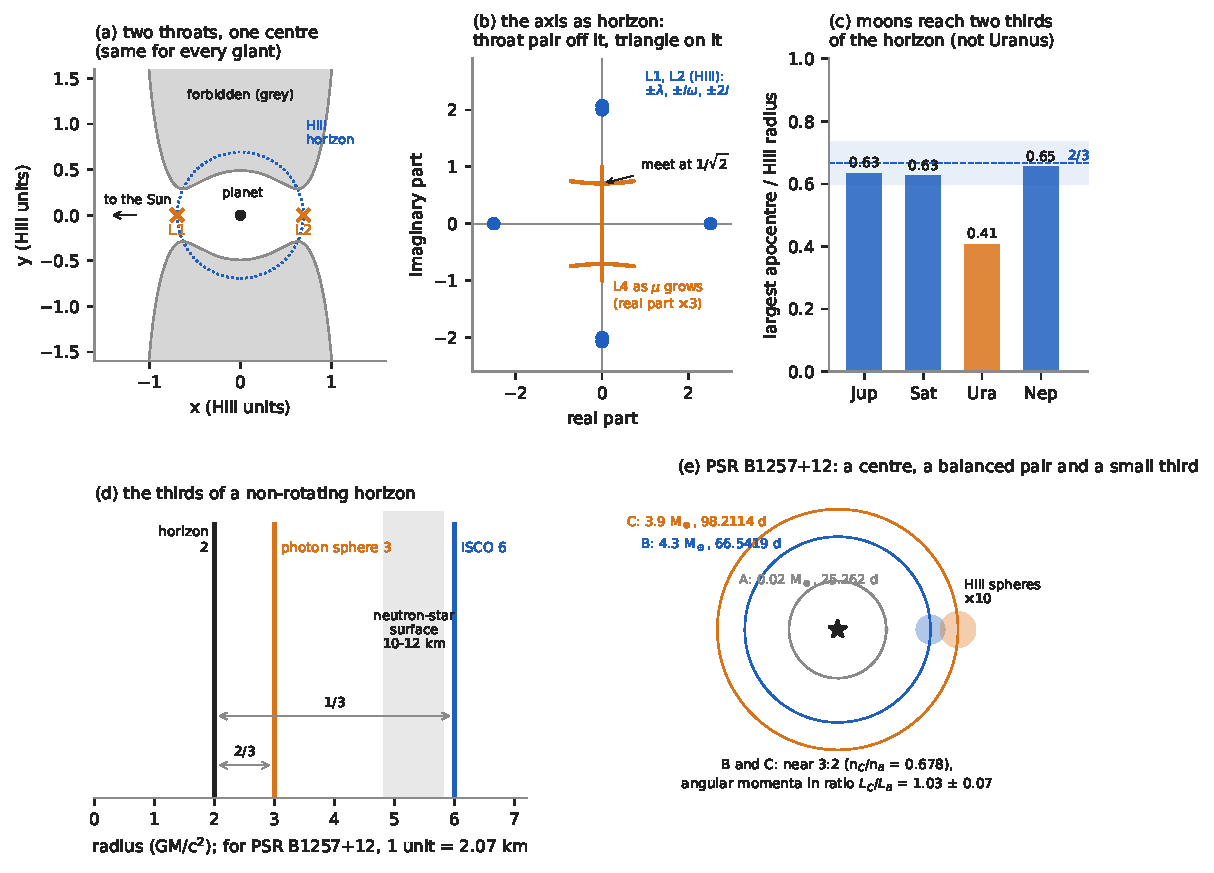
\includegraphics[width=0.93\textwidth]{fig_throats.pdf}
\caption{(a) The zero-velocity curve in Hill's units at $C=3^{4/3}-0.25$, below the throat value: the planet's realm opens towards the Sun at $L_1$ and outwards at $L_2$; dotted, the Hill radius. (b) Blue: the throat spectrum, a real pair $\pm\lambda$ off the imaginary axis and two pairs on it. Orange: the $L_4$ spectrum as $\mu$ grows from $10^{-5}$ to $0.06$; the two pairs meet at $1/\sqrt2$ and leave the axis as a quadruple (real parts drawn three times larger). (c) The largest apocentre of each giant's known moons against its Hill radius; the band marks $0.600$--$0.733$, within $10\%$ of $\frac23$. (d) Schwarzschild radii in units of $GM/c^2$; grey, neutron-star radii of $10$--$12$ km for $1.4\,M_\odot$. (e) The planets of PSR~B1257+12, with Hill spheres enlarged tenfold.}\label{fig:throats}
\end{figure}

\section{The hearts}\label{sec:hearts}
Juno's radio tracking gives Jupiter's gravity field and its infrared mapper watches the poles \cite{Durante2020,Durante2022,Adriani}. Cassini's Grand Finale in 2017 flew between Saturn and its rings and gave Saturn's field \cite{Iess}; earlier, its stellar occultations recorded $17$ density waves and $4$ bending waves in the C ring driven by Saturn's own oscillations \cite{Mankovich2019}.

\subsection{The rotational response}\label{sec:love}
The response of $J_2$ to the spin measures how strongly mass gathers to the centre. For a uniform sphere $J_2/q_\omega=\frac12$; for the $n=1$ polytrope it follows exactly from the Love number.

\begin{proposition}[the $n=1$ polytrope]\label{prop:love}
For the polytrope $P=K\rho^2$ of mass $M$ and radius $R$, $\rho=\rho_c\sin u/u$ with $u=\pi r/R$, $\rho_c=\pi M/4R^3$ and $K=2GR^2/\pi$. Its fluid Love number is $k_2=15/\pi^2-1=0.519818$, and to first order in the rotation $J_2=\frac13k_2q_\omega$, so that $J_2/q_\omega=(15/\pi^2-1)/3=0.17327$.
\end{proposition}
\begin{proof}
Let $W$ be an applied potential with $\nabla^2W=0$ inside the body and $\Phi$ the self-potential. Hydrostatic equilibrium $\nabla P=-\rho\nabla(\Phi+W)$ with $P=K\rho^2$ gives $2K\nabla\rho=-\nabla(\Phi+W)$, so $2K\rho+\Phi+W$ is constant, and Poisson's equation $\nabla^2\Phi=4\pi G\rho$ becomes $\nabla^2\Phi+k^2\Phi=k^2(c-W)$ with $k^2=2\pi G/K$. For $W=0$ the regular solution gives $\rho\propto\sin(kr)/(kr)$, which first vanishes at $kR=\pi$; hence $K=2GR^2/\pi$, and $M=4\pi\rho_c(R/\pi)^3\,\pi$ gives $\rho_c=\pi M/4R^3$. Now let $W=wr^2P_2(\cos\theta)$ and write $\Phi_1$ for the change of the self-potential. Inside, $\nabla^2\Phi_1+k^2\Phi_1=-k^2W$, whose regular solution is $\Phi_1=[-wr^2+A\,j_2(kr)]P_2$, with $j_2$ the spherical Bessel function; outside, $\Phi_1=Br^{-3}P_2$. The unperturbed density vanishes at $r=R$, so the displaced surface carries no mass at first order and $\Phi_1$ and $\partial_r\Phi_1$ are continuous there. With $j_2(\pi)=3/\pi^2$ and $j_2'(\pi)=j_1(\pi)-\frac3\pi j_2(\pi)=\frac1\pi-\frac9{\pi^3}$, matching gives
\[
-wR^2+A\tfrac3{\pi^2}=BR^{-3},\qquad -2wR+A\tfrac\pi R\bigl(\tfrac1\pi-\tfrac9{\pi^3}\bigr)=-3BR^{-4}.
\]
Adding $3/R$ times the first equation to the second eliminates $B$ and leaves $-5wR+A/R=0$, so $A=5wR^2$ and $BR^{-3}=wR^2(15/\pi^2-1)$: the response at the surface is $k_2=15/\pi^2-1$ times the applied potential. For uniform rotation the centrifugal potential $-\frac12\omega_\mathrm{rot}^2r^2\sin^2\theta$ has quadrupole part $w=\omega_\mathrm{rot}^2/3$. Outside, the response $k_2\frac{\omega_\mathrm{rot}^2}3R^5r^{-3}P_2$ is the $J_2$ term $GMJ_2R^2r^{-3}P_2$ of the exterior potential $-\frac{GM}r[1-J_2(\frac Rr)^2P_2]$, so $J_2=k_2\omega_\mathrm{rot}^2R^3/3GM=\frac13k_2q_\omega$.
\end{proof}

All four giants lie below $0.17327$ (\cref{tab:giants}): Jupiter at $0.16477$, Saturn at $0.10303$, Uranus at $0.11331$ and Neptune at $0.13080$. Saturn is the most centrally condensed. The polytropic index for which first-order Clairaut theory on the Lane--Emden profile reproduces the measured $J_2/q_\omega$ is $1.04$ for Jupiter and $1.44$ for Saturn. The first-order Radau--Darwin relation, $I/MR^2=\frac23\bigl[1-\frac25\sqrt{\eta-1}\bigr]$ with $\eta=5q_\omega/(3J_2+q_\omega)$ \cite{MilitzerHubbard2023}, gives the moments of inertia in \cref{tab:giants}, against $\frac25$ for a uniform sphere; it assumes a nearly uniform density and is least reliable for strongly layered planets.

\subsection{The heart of Jupiter}\label{sec:jupheart}
Juno measured $J_2=14696.5735$, $J_4=-586.6085$ and $J_6=34.2007$ ($\times10^{-6}$, reference radius $71492$ km) \cite{Durante2020}. Interior models fitted to Juno's field place a dilute core between $0.3$ and $0.5$ of the radius \cite{Wahl}. In the five-layer reference model of Militzer and Hubbard the dilute core extends to $0.42$ and a stably stratified transition layer to $0.62$ of the radius, spanning the cumulative mass fractions $0.20$ to $0.54$; any compact core weighs at most $2.5$ (rock) to $3.0$ (rock--ice) Earth masses of the $23.5$--$25.5$ Earth masses of heavy elements \cite{Militzer2024}. The zonal winds reach about $3000$ km down, $4\%$ of the radius \cite{Kaspi2018,Kaspi2020}.

\paragraph{The heartbeat.} Juno's Doppler record carries residuals of up to $0.1$ mm/s over $10$--$15$ minutes in its $22$ gravity passes, which resist a low-order static interpretation; they are fitted by pressure modes (p-modes) at $900$--$1200\muH$ with surface speeds of $10$--$50$ cm/s and displacements of $15$--$80$ m \cite{Durante2022}. From the ground, Jupiter's oscillations peak at $1213\pm50\muH$ with a spacing of $155.3\pm2.2\muH$ \cite{Gaulme}. The spacing is set by the sound-crossing time, $\Delta\nu=[2\int_0^R\dd r/c]^{-1}$. In the $n=1$ polytrope with $\Gamma_1=2$, \cref{prop:love} gives
\[
c^2=\Gamma_1\frac P\rho=\Gamma_1K\rho=\frac{\Gamma_1GM}{2R}\,\frac{\sin u}{u},\qquad
\int_0^R\frac{\dd r}{c}=\frac R\pi\Bigl(\frac{2R}{\Gamma_1GM}\Bigr)^{1/2}\int_0^\pi\Bigl(\frac u{\sin u}\Bigr)^{1/2}\dd u ,
\]
and the last integral is $5.893400$ by quadrature. With $\Gamma_1=2$, $\Delta\nu=\frac{\pi^2}{5.893400}\,\nu_\mathrm{dyn}=1.6747\,\nu_\mathrm{dyn}$, where $\nu_\mathrm{dyn}=(GM/R^3)^{1/2}/2\pi$ is the planet's dynamical frequency. For Jupiter ($R=69911$ km, the volumetric mean radius) the crossing takes $3081$ s and $\Delta\nu=162.3\muH$, $4.5\%$ above the measurement, from mass and radius alone.

\subsection{The heart of Saturn and the signal in the tracking}\label{sec:saturnheart}
Cassini measured $J_2=16290.573$, $J_4=-935.314$ and $J_6=86.340$ ($\times10^{-6}$, reference radius $60330$ km) \cite{Iess}. The same tracking held a signal that the gravity solution could not absorb: range-rate residuals of up to $0.2$ mm/s over $20$--$60$ minutes, accelerations of order $10^{-7}$ m/s$^2$, handled in the published field by random accelerations in $10$-minute steps near closest approach \cite{Iess}. A forward model of Saturn's normal modes reproduces it, favouring p-modes at $500$--$700\muH$ with amplitudes of several kilometres; no single fundamental mode had more than a $2\%$ chance of producing it, and the corresponding signal at Jupiter is about $20$ times weaker \cite{Markham}. This is the gravitational anomaly in the data around Saturn, and its reading is Saturn's own ringing, recorded by the spacecraft that flew through it.

\paragraph{In the rings.} The ring-wave pattern speeds, known to better than $0.1$ deg/day, fixed Saturn's day at $10^\mathrm{h}33^\mathrm{m}38^\mathrm{s}$, with the $5\%$ and $95\%$ quantiles $1^\mathrm{m}19^\mathrm{s}$ below and $1^\mathrm{m}52^\mathrm{s}$ above \cite{Mankovich2019}. The gravity-mode waves fixed its heart: a stably stratified core out to $0.59\pm0.01$ of the radius (linear composition profile) or $0.70\pm0.02$ (smooth profile), half of the heavy elements within $0.32\pm0.01$, and $19.1\pm1.0$ Earth masses of heavy elements, $17.4\pm1.2$ of them in the stable region \cite{MankovichFuller}.

\subsection{What links the two hearts}\label{sec:links}
\paragraph{One pressure.} Jupiter's winds are inferred to end near $3000$ km and Saturn's near $9000$ km, and both depths lie near $10^5$ bar \cite{Kaspi2020}, where hydrogen's conductivity reaches about $1$ S/m and the magnetic field is expected to brake the flow \cite{Kaspi2020,Galanti}. In the $n=1$ polytrope of \cref{prop:love} ($\rho_c=4363$ and $2260$ kg/m$^3$) the pressure $P=K\rho^2$ is $7.899\times10^4$ bar at $3000$ km in Jupiter and $2.273\times10^5$ bar at $9000$ km in Saturn, and the $10^5$ bar level lies at $3360$ and $6180$ km. In polytropes whose first-order $J_2/q_\omega$ matches each planet ($n=1.04$ and $1.44$) the pressures are $6.908\times10^4$ and $1.070\times10^5$ bar, and the $10^5$ bar level lies at $3569$ and $8786$ km (\cref{fig:heart}b); the mid-point of Saturn's inferred wind decay is at $8743$ km \cite{Galanti}. Saturn's greater central condensation therefore brings the two depths to one pressure: the ratio of the pressures falls from $2.88$ ($n=1$) to $1.55$. The depth ratio of the $10^5$ bar level, $2.46$, follows mostly from the surface gravities, $24.79$ and $10.44$ m/s$^2$ (ratio $2.37$), since layers of one material reach a given pressure at depths in the inverse ratio of $g$. One physical level, found in two planets at depths near the inverse ratio of their gravities, is the equivalence that links their winds.

\paragraph{One heartbeat.} Both planets carry tracking signals best read as p-modes \cite{Durante2022,Markham}. Each planet's natural clock is $\nu_\mathrm{dyn}$: $96.91\muH$ for Jupiter and $69.75\muH$ for Saturn, ratio $1.3893$. The ratios of the published p-mode bands (Juno $900$--$1200$, Cassini $500$--$700\muH$) run from $1.286$ to $2.400$, so the bands are consistent with each planet ringing on its own clock. Scaled from Jupiter's measured spacing by $\nu_\mathrm{dyn}$, Saturn's acoustic spacing is $111.8\muH$; the $n=1$ polytrope gives $116.8\muH$. We predict Saturn's spacing at $112$--$117\muH$; a long, continuous record of Saturn's disk or gravity would measure it.

\paragraph{One shape of heart.} Both planets hold their heavy elements in a dilute, stratified core (\cref{fig:heart}a). In Saturn half of them lie within $0.32\pm0.01$ of the radius, $1.33\sigma$ from one third, and the stable region ends at $0.59\pm0.01$ or $0.70\pm0.02$, $7.67\sigma$ below and $1.67\sigma$ above two thirds. In Jupiter the dilute core and the transition layer reach $0.42$ and $0.62$.

\subsection{The poles: a centre and its ring}\label{sec:poles}
Jupiter's north pole has eight cyclones around one, its south pole five around one \cite{Adriani}. On 4 November 2019 a sixth joined the southern ring \cite{PIA}; it was gone two months later \cite{Mura}. The classical model is a ring of $N$ point vortices of strength $1$ at radius $1$ around a central vortex of strength $\kappa$, rotating rigidly at $\Omega_N=((N-1)/2+\kappa)/2\pi$ \cite{Thomson}. We computed its linear stability, with the central vortex free to move, from the analytic Jacobian in the co-rotating frame, which agrees with finite differences to $9.55\times10^{-10}$ (\cref{fig:heart}c). Thomson's heptagon ($N=7$, no centre) is neutral (largest growth rate $9.9\times10^{-9}$), and eight without a centre grow at $0.450$. For $N=4,\dots,12$ the computed intervals of spectral stability coincide, to $4\times10^{-11}$ at both edges, with those of Cabral and Schmidt's theorem \cite{Cabral,BHW},
\[
\frac{N^2-8N+8}{16}<\kappa<\frac{(N-1)^2}4\ (N\ \text{even}),\qquad \frac{(N-1)(N-7)}{16}<\kappa<\frac{(N-1)^2}4\ (N\ \text{odd}).
\]
For $N=3$ the upper edge is $\kappa=1$ and no lower edge lies above $-20$. At the upper edge the centre holds the share $\kappa/(\kappa+N)=(N-1)^2/((N-1)^2+4N)=((N-1)/(N+1))^2$ of the total strength.
\begin{itemize}
\item \emph{Three with an equal fourth sit on the edge.} For $N=3$, $\kappa_{\max}=1$: an equal fourth vortex at the centre of three leaves the triad exactly marginal. The growth rate is zero below $\kappa=1$, $5.0\times10^{-3}$ at $1.001$ and $1.6\times10^{-2}$ at $1.01$, rising as $\sqrt{\kappa-1}$.
\item \emph{Large rings need a centre.} For $N\ge8$ the lower edge is positive. Jupiter's northern $8+1$ with an equal centre has central share $\frac19$, inside its interval $[0.059,0.605]$ (largest growth rate $1.0\times10^{-8}$).
\item \emph{The south.} With equal centres, $5+1$ and $6+1$ are both inside their intervals (growth rates $6.6\times10^{-9}$ and $1.9\times10^{-16}$), so the departure of the sixth cyclone is set by what the planar model leaves out: on the planet each cyclone is wrapped in a shielding ring of opposite vorticity \cite{Li}, and the ring of cyclones sits on a curved pole at $83^\circ$, $8700$ km from the centre \cite{Chen}.
\end{itemize}

\paragraph{Saturn's poles and hemispheres.} In the north, the hexagon's vertices lie at $74.7^\circ$ planetocentric latitude and turn in $10^\mathrm{h}39^\mathrm{m}23.01^\mathrm{s}$; its $120$ m/s jet survived the polar night \cite{SLHex}. In the south, a ten-sided wave formed at $63^\circ$S: faint in October 2023, sharper in August 2024, complete with ten vertices in August--September 2025 \cite{SLDec}, in the months after the Sun crossed the ring plane on 6 May 2025 \cite{AAQ}; its winds are reported as about $400$ km/h \cite{SSL}. Saturn's northern and southern radio emissions pulse with their own periods, about $10.6$ and $10.8$ hours before the 2009 equinox; the two converged, crossed shortly after the equinox of 11 August 2009, and merged near $10.7$ hours in spring 2010 \cite{Fischer}. The opposite hemispheres, one on each side of the ring plane, joined in one period in the months after the Sun crossed that plane. Saturn's magnetic dipole is tilted by less than $0.007^\circ$ from its spin axis \cite{Cao}.

\paragraph{Jupiter's poles in X-rays.} Chandra's High Resolution Camera found the northern auroral X-ray hot spot pulsing with a period of about $45$ minutes on 18 December 2000 \cite{Gladstone}. XMM-Newton and Chandra campaigns in March 2007 and May--June 2016 found the southern X-ray aurora pulsing every $11$ minutes while the northern aurora varied independently of it \cite{Dunn}. The two poles are a pair whose pulses are not locked to each other.

\begin{figure}[!htb]
\centering
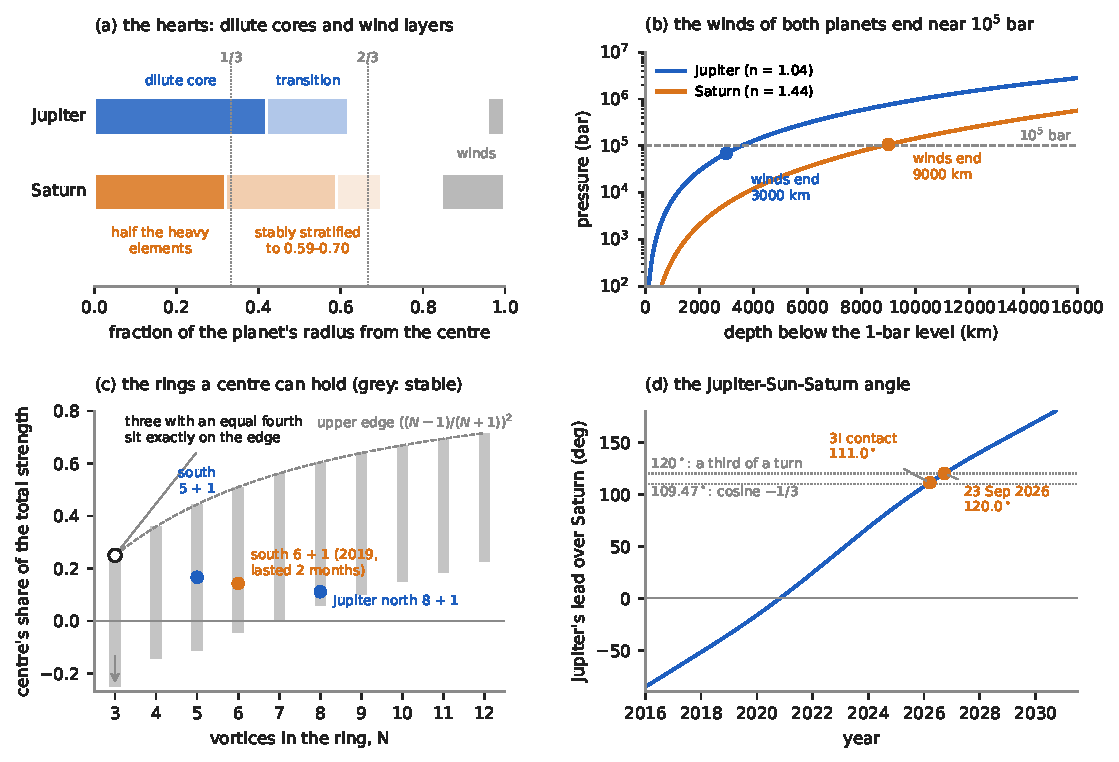
\includegraphics[width=\textwidth]{fig_heart.pdf}
\caption{(a) The hearts by fraction of radius: Jupiter's dilute core and transition layer \cite{Militzer2024}, Saturn's heavy-element core and stable region \cite{MankovichFuller}, and the wind layers (grey); dotted lines at $\frac13$ and $\frac23$. (b) Pressure against depth in the polytropes whose $J_2/q_\omega$ matches each planet; dots mark the published wind depths. (c) Grey: the central share $\kappa/(\kappa+N)$ for which a ring of $N$ equal vortices around a centre of strength $\kappa$ is spectrally stable; dashed, the upper edge $((N-1)/(N+1))^2$; dots, Jupiter's polar patterns with the centre equal to the others. (d) Jupiter's lead over Saturn in heliocentric longitude, with the 3I/ATLAS contact of \cref{sec:contact}.}
\label{fig:heart}
\end{figure}

\section{The gas ladder}\label{sec:ladder}
Each giant's troposphere is a ladder of cloud decks. Water condenses deepest; above it ammonia and hydrogen sulfide combine into solid ammonium hydrosulfide; above that the survivor of that reaction condenses as ice; and in the two cold planets methane condenses on top. The equilibrium cloud-condensation model that computes this ladder goes back to Lewis and to Weidenschilling and Lewis \cite{Lewis1969,WL73}; its modern form is that of Atreya and Wong \cite{AtreyaWong}. We build it from stated thermodynamic data, validate it against the published decks, and show that its middle rung is an exact two-state pair whose balance decides what each planet shows above its clouds.

\subsection{Inputs}\label{sec:ladderinputs}
\Cref{tab:ladderinputs} lists every external input. The deck bases depend on the $1$-bar temperature, the abundances of the condensing species, the saturation vapour pressures and the heat capacity of the gas; the gravity enters only the conversion from pressure to altitude.

\begin{table}[!htb]\centering\footnotesize
\begin{tabular}{@{}>{\raggedright\arraybackslash}p{3.0cm}>{\raggedright\arraybackslash}p{8.1cm}>{\raggedright\arraybackslash}p{3.8cm}@{}}\toprule
input & value & source\\\midrule
$T$ at $1$ bar & Jupiter $165$ K, Saturn $134$ K, Uranus $76$ K, Neptune $72$ K & NSSDC \cite{NSSDCJ,NSSDCS,NSSDCU,NSSDCN}\\
gravity at $1$ bar & $23.12$, $8.96$, $8.69$, $11.00$ m\,s$^{-2}$ (equatorial) & NSSDC\\
$T$ at $0.1$ bar (context) & $112$, $84$, $53$, $55$ K & NSSDC\\
bulk composition (context) & J: H$_2$ $89.8\%$, He $10.2\%$; S: $96.3\%$, $3.25\%$; U: $82.5\%$, $15.2\%$, CH$_4$ $2.3\%$; N: $80.0\%$, $19.0\%$, CH$_4$ $1.5\%$ & NSSDC\\
protosolar X/H & C $2.95\times10^{-4}$, N $7.41\times10^{-5}$, O $5.37\times10^{-4}$, S $1.45\times10^{-5}$ (N/S $=5.110$) & \cite{Asplund2009}, photospheric $+0.04$ dex, as tabulated in \cite{Atreya2020}\\
He/H$_2$ & J $0.157$; S $0.135$ (alternative $0.124$); U $0.180$; N $0.241$ ($0.180$ with N$_2$) & \cite{Atreya2020}\\
Jupiter NH$_3$ & $362\pm33$ ppmv (nominal); $351^{+22}_{-21}$ ppmv; Galileo probe N/H $=(3.32\pm1.27)\times10^{-4}$ ($566\pm216$ ppmv); depleted $100$--$250$ ppmv at mid-latitudes & \cite{Li2017,Li2020,Wong2004,Guillot2020b}\\
Jupiter H$_2$S & S/H $=(4.45\pm1.05)\times10^{-5}$ (H$_2$S/H$_2=(8.9\pm2.1)\times10^{-5}$) & \cite{Wong2004}\\
Jupiter H$_2$O & $2.5^{+2.2}_{-1.6}\times10^3$ ppmv at $0$--$4^\circ$N; $490\pm160$ ppmv in the $5$-$\mu$m hot spot & \cite{Li2020,Wong2004}\\
Jupiter CH$_4$ & C/H $=1.19\times10^{-3}$ & \cite{Wong2004}, via \cite{Atreya2020}\\
Saturn CH$_4$, NH$_3$ & $(4.7\pm0.2)\times10^{-3}$; $(4\pm1)\times10^{-4}$ (observed to $3$ bar) & \cite{Fletcher2009,Atreya2020}\\
Saturn S, O & S: $1\times$ protosolar to S/H $=1.88\times10^{-4}$ ($13\times$, marked highly uncertain by the compilers), nominal $5\times$; O: $1$--$10\times$, nominal $5\times$ & \cite{Atreya2020,AtreyaWong}\\
Uranus NH$_3$, H$_2$S & deep $1.7^{+0.7}_{-0.4}\times10^{-4}$ and $8.7^{+3.1}_{-1.5}\times10^{-4}$, N/S $=0.20^{+0.08}_{-0.07}$; above the cloud $0.4$--$0.8$ ppm H$_2$S at the $1.2$--$3$ bar cloud top, below it $>(1.0$--$2.5)\times10^{-5}$ & \cite{Molter2021,Irwin2018}\\
Neptune H$_2$S & $1$--$3$ ppm at the $2.5$--$3.5$ bar cloud tops, below the cloud $>(0.4$--$1.3)\times10^{-5}$; deep H$_2$S $10$--$30\times$ solar, bulk S/N $>5\times$ solar & \cite{Irwin2019a,dePater1991}\\
Uranus, Neptune CH$_4$ & $\approx4\%$ (equatorial) to $\approx2\%$ (polar) near the $2$--$3$ bar cloud tops & \cite{Irwin2019b}\\
ice-giant H$_2$O & $1$, $10$, $30$, $80\times$ protosolar; nominal $30\times$ & \cite{Atreya2020,Molter2021}\\
NH$_4$SH equilibrium & $\log_{10}(P_{\NH}P_{\HS}/\mathrm{atm}^2)=14.82-4705/T$ & \cite{AtreyaWong}, eq.~(3)\\
H$_2$ constants & $\omega_e=4401.213$, $\omega_ex_e=121.336$, $B_e=60.8530$, $\alpha_e=3.0622$, $D_e=0.0471$ cm$^{-1}$ & \cite{HuberHerzberg}, via \cite{NISTWebBook}\\
H$_2$ heat capacity (validation) & normal and para H$_2$, $0.1$ bar, $40$--$400$ K & \cite{Leachman}, via \cite{NISTWebBook}\\
H$_2$O vapour pressure & liquid: IAPWS SR1-86, $T_c=647.096$ K, $p_c=22.064$ MPa; ice Ih: IAPWS R14-08, $T_t=273.16$ K, $p_t=611.657$ Pa & \cite{WagnerPruss,Wagner2011}\\
NH$_3$ & $T_\mathrm{fus}=194.95$ K, $P_\mathrm{triple}=0.06060$ bar, $\Delta_\mathrm{sub}H=31.2$ kJ\,mol$^{-1}$; Antoine $3.18757-506.713/(T-80.78)$ ($164$--$239.6$ K), $4.86886-1113.928/(T-10.409)$ ($239.6$--$371.5$ K), $\log_{10}P/$bar & \cite{NISTWebBook}\\
H$_2$S & $T_\mathrm{triple}=187.66$ K, $P_\mathrm{triple}=0.232$ bar, $T_\mathrm{boil}=212.87$ K; $\Delta_\mathrm{sub}H=22.5$ kJ\,mol$^{-1}$ at $135$ K, $25.4$ at $175$ K; Antoine $4.43681-829.439/(T-25.412)$ ($138.8$--$212.8$ K), $4.52887-958.587/(T-0.539)$ ($212.8$--$349.5$ K) & \cite{NISTWebBook}\\
CH$_4$ & $T_\mathrm{triple}=90.67$ K, $P_\mathrm{triple}=0.1169$ bar; $\Delta_\mathrm{sub}H=9.7$ kJ\,mol$^{-1}$ at $72$ K; liquid Antoine $3.9895-443.028/(T-0.49)$ ($90.99$--$189.99$ K) & \cite{NISTWebBook}\\
constants & $R=8.314462618$ J\,mol$^{-1}$K$^{-1}$, $hc/k_B=1.438776877$ cm\,K & \cite{CODATA}\\\bottomrule
\end{tabular}
\caption{Inputs of the gas ladder. The NIST WebBook compiles the NH$_3$, H$_2$S and CH$_4$ data from their primary sources, listed in \cref{sec:data}.}\label{tab:ladderinputs}
\end{table}

\subsection{The model}\label{sec:model}
\paragraph{(i) Composition.} Deep mole fractions $x_i$ of the trace species are given either directly (Juno, Molter et al., Fletcher et al., ice-giant CH$_4$) or as ratios $r_i$ to H$_2$ (Galileo, protosolar multiples). Then
\[
x_\mathrm{H_2}=\frac{1-\sum_\mathrm{given}x_j}{1+\mathrm{He/H_2}+\sum_ir_i},\qquad x_\mathrm{He}=(\mathrm{He/H_2})\,x_\mathrm{H_2},\qquad x_i=r_i\,x_\mathrm{H_2}.
\]
The nominal abundances are, for Jupiter, NH$_3$ $362$ ppmv (Juno), H$_2$S/H$_2=8.9\times10^{-5}$ (Galileo) and H$_2$O $2500$ ppmv (Juno); for Saturn, NH$_3$ $4\times10^{-4}$ and S and O at $5\times$ protosolar; for Uranus, the NH$_3$ and H$_2$S of Molter et al., CH$_4$ $4\%$ and O $30\times$ protosolar; for Neptune, N $1\times$, S $30\times$ and O $30\times$ protosolar, CH$_4$ $4\%$. They give the mole fractions of \cref{tab:mole}. We write $\mathrm N=x_{\NH}$ and $\mathrm S=x_{\HS}$ for the deep values.

\begin{table}[!htb]\centering\footnotesize\setlength{\tabcolsep}{4pt}
\begin{tabular}{@{}lcccccccc@{}}\toprule
 & H$_2$ & He & CH$_4$ & NH$_3$ & H$_2$S & H$_2$O & N/S & $\Delta=\mathrm N-\mathrm S$\\\midrule
Jupiter & $0.8600$ & $0.1350$ & $2.047\times10^{-3}$ & $3.620\times10^{-4}$ & $7.654\times10^{-5}$ & $2.500\times10^{-3}$ & $4.730$ & $+2.855\times10^{-4}$\\
Saturn & $0.8723$ & $0.1178$ & $4.700\times10^{-3}$ & $4.000\times10^{-4}$ & $1.265\times10^{-4}$ & $4.684\times10^{-3}$ & $3.162$ & $+2.735\times10^{-4}$\\
Uranus & $0.7911$ & $0.1424$ & $0.0400$ & $1.700\times10^{-4}$ & $8.700\times10^{-4}$ & $2.549\times10^{-2}$ & $0.1954$ & $-7.000\times10^{-4}$\\
Neptune & $0.7534$ & $0.1816$ & $0.0400$ & $1.117\times10^{-4}$ & $6.555\times10^{-4}$ & $2.427\times10^{-2}$ & $0.1703$ & $-5.438\times10^{-4}$\\\bottomrule
\end{tabular}
\caption{Nominal deep mole fractions. $\mathrm{N/S}=x_{\NH}/x_{\HS}$ at depth; protosolar N/S is $5.11$.}\label{tab:mole}
\end{table}

\paragraph{(ii) The heat capacity of hydrogen, and its ortho/para state.} Take the rotational levels of the vibrational ground state, $E_J/hc=B_0J(J+1)-D_e[J(J+1)]^2$ with $B_0=B_e-\alpha_e/2=59.3219$ cm$^{-1}$, which gives $E_1=118.455$, $E_2=354.236$, $E_3=705.080$ and $E_4=1167.60$ cm$^{-1}$; we keep $J\le15$, where the levels still increase. The nuclear-spin weights are $1$ for para (even $J$) and $3$ for ortho (odd $J$), times $2J+1$. For levels with weights $g_J$ and reduced energies $x_J=hcE_J/k_BT$, the rotational heat capacity is the variance $\mathrm{Var}(x)$ under the weights $g_J\e^{-x_J}$ (the second derivative of $\ln Z$ in $1/T$). Then,
for normal H$_2$, with ortho:para frozen at $3{:}1$,
\[
\frac{c_p}R=\frac52+\frac14\mathrm{Var}_\mathrm{para}+\frac34\mathrm{Var}_\mathrm{ortho}+c_\mathrm{vib},
\]
and for equilibrium H$_2$
\[
\frac{c_p}R=\frac52+\mathrm{Var}_\mathrm{all}+c_\mathrm{vib},
\]
where the second includes the heat of ortho--para conversion and $c_\mathrm{vib}$ is the harmonic term for the fundamental interval $\omega_e-2\omega_ex_e=4158.541$ cm$^{-1}$. Against the NIST fluid data at $0.1$ bar and $40$--$400$ K \cite{Leachman}, the computed $c_p$ agrees to $0.24\%$ for normal H$_2$ ($22.565$ against $22.578$ J\,mol$^{-1}$K$^{-1}$ at $100$ K) and to $0.24\%$ for para H$_2$ ($27.007$ against $27.015$). No single value of $c_p$ fits the tropospheres, which span $70$--$600$ K (\cref{tab:cp}). The nominal model uses normal H$_2$ with $c_p(T)$ from these levels, He with $c_p/R=\frac52$ and the polyatomic vapours as rigid non-linear rotors, $c_p/R=4$.

\begin{table}[!htb]\centering\footnotesize\setlength{\tabcolsep}{4pt}
\begin{tabular}{@{}lccccccccccc@{}}\toprule
$T$ (K) & $60$ & $76$ & $80$ & $100$ & $120$ & $140$ & $165$ & $200$ & $300$ & $400$ & $600$\\\midrule
normal & $2.519$ & $2.571$ & $2.590$ & $2.714$ & $2.857$ & $2.993$ & $3.135$ & $3.280$ & $3.470$ & $3.511$ & $3.529$\\
equilibrium & $4.359$ & $3.853$ & $3.747$ & $3.386$ & $3.232$ & $3.191$ & $3.217$ & $3.302$ & $3.471$ & $3.511$ & $3.529$\\\bottomrule
\end{tabular}
\\[4pt]
\begin{tabular}{@{}lccc@{}}\toprule
$R/\bar c_p$ at $1$ bar & normal H$_2$ & equilibrium H$_2$ & mean molar mass (g\,mol$^{-1}$)\\\midrule
Jupiter & $0.3278$ & $0.3203$ & $2.318$\\
Saturn & $0.3442$ & $0.3209$ & $2.317$\\
Uranus & $0.3884$ & $0.2740$ & $2.453$\\
Neptune & $0.3922$ & $0.2713$ & $2.458$\\\bottomrule
\end{tabular}
\caption{Top: $c_p/R$ of normal and equilibrium H$_2$. Bottom: the adiabatic exponent of each mixture at $1$ bar.}\label{tab:cp}
\end{table}

\paragraph{(iii) Dry adiabat.} For an ideal mixture with molar heat capacity $\bar c_p(T)=\sum_ix_ic_{p,i}(T)$ over the local gas,
\[
\frac{\dd\ln T}{\dd\ln P}=\frac R{\bar c_p(T)},\qquad T(1\ \mathrm{bar})=T_\mathrm{NSSDC},
\]
integrated upward to $0.2$ bar and downward to $300$ bar (Jupiter, Saturn) or $3000$ bar (Uranus, Neptune) by the fourth-order Runge--Kutta method in $\ln P$ with step $0.002$. Condensable vapours above their decks are held at their local saturation values in $\bar c_p$. Anchored at the Galileo $1$-bar temperature of $166.1$ K, the Jupiter adiabat gives $426.65$ K at $22$ bar; the probe measured $427.7\pm1.5$ K (Seiff et al., as quoted in \cite{Guillot2020b}).

\paragraph{(iv) Saturation vapour pressures.} Water follows the IAPWS liquid equation above $273.16$ K and the IAPWS ice-Ih sublimation equation below, with no condensation above $647.096$ K \cite{WagnerPruss,Wagner2011}. Solid NH$_3$, H$_2$S and CH$_4$ follow the Clausius--Clapeyron law through the triple point with constant sublimation enthalpy, $p_\mathrm{sat}=p_t\exp[-\frac LR(\frac1T-\frac1{T_t})]$, with $(T_t,p_t,L)=(194.95\ \mathrm K,0.06060\ \mathrm{bar},31.2\ \mathrm{kJ\,mol^{-1}})$, $(187.66,0.232,22.5)$ and $(90.67,0.1169,9.7)$; liquids above their triple points follow the Antoine equations of \cref{tab:ladderinputs}. As sensitivity variants we extrapolate Stull's solid-range Antoine equations below their lower limits (the NH$_3$ form diverges near $81$ K and is spliced to the Clausius--Clapeyron shape below $120$ K, far from any deck base), use $L=25.4$ kJ\,mol$^{-1}$ for H$_2$S, and vary $L$ of CH$_4$ by $\pm5\%$. The adopted and Stull curves give, for NH$_3$, $1.89\times10^{-4}$ against $7.37\times10^{-5}$ bar at $164$ K and $1.60\times10^{-3}$ against $1.26\times10^{-3}$ bar at $180$ K; for H$_2$S, $6.83\times10^{-5}$ (adopted), $4.65\times10^{-5}$ (Stull) and $2.39\times10^{-5}$ bar ($L=25.4$) at $120$ K, and $1.71\times10^{-3}$ against $1.58\times10^{-3}$ bar at $140$ K.

\paragraph{(v) The NH$_4$SH equilibrium.} $\NH(\mathrm g)+\HS(\mathrm g)\rightleftharpoons\NHSH(\mathrm s)$ with $K(T)=P_{\NH}P_{\HS}$ in atm$^2$ and $\log_{10}K=14.82-4705/T$ \cite{AtreyaWong}; the NH$_3$--H$_2$S cloud chemistry goes back to Lewis \cite{Lewis1969}. The van 't Hoff enthalpy is $L_\mathrm{rx}=4705\,R\ln10=90.08$ kJ\,mol$^{-1}$, and $\dd\ln K/\dd T=10834/T^2$; for example $K(200\ \mathrm K)=1.97\times10^{-9}$ and $K(250\ \mathrm K)=1.00\times10^{-4}$ atm$^2$.

\paragraph{(vi) The deck base as a balance point.} For a simple condensable with vapour mole fraction $x$, define the log saturation ratio
\[
\varepsilon_\mathrm{deck}(P)=\ln\frac{xP}{p_\mathrm{sat}(T(P))}.
\]
Condensate is stable where $\varepsilon_\mathrm{deck}>0$, and the deck base is the deepest level where $\varepsilon_\mathrm{deck}=0$, crossing from negative below to positive above; we find it by root bracketing on the profile. For NH$_4$SH, $\varepsilon_{\NHSH}=\ln(x_{\NH}x_{\HS}P_\mathrm{atm}^2/K(T))$. For the ice deck of the surviving species (NH$_3$ or H$_2$S), $x$ is the mole fraction left by the NH$_4$SH equilibrium at that level (\cref{sec:titration}). Each deck is thus a two-state pair, vapour and condensate, and its base is the balance point where the saturation ratio is $1$, $\varepsilon_\mathrm{deck}=0$.

\paragraph{(vii) Moist pseudo-adiabat (sensitivity).} Let $L_k=RT^2\dd\ln p_{\mathrm{sat},k}/\dd T$ be the latent heats of the saturated species. The first law for one mole of gas reads $\bar c_p\dd T-RT\dd\ln P=-\sum_kL_k\dd x_k-L_\mathrm{rx}\dd x_{\HS}$. For a saturated species $x_kP=p_{\mathrm{sat},k}(T)$, so $\dd x_k=x_k(L_k\dd T/RT^2-\dd\ln P)$. For NH$_4$SH, $x_{\NH}x_{\HS}P^2=K$ and the two gases are removed $1{:}1$, so $\dd x_{\NH}=\dd x_{\HS}=Y(10834\,\dd T/T^2-2\dd\ln P)$ with $Y=x_{\NH}x_{\HS}/(x_{\NH}+x_{\HS})$; this counts the reaction heat once per pair removed. Substituting and solving for $\dd\ln T/\dd\ln P$ gives
\[
\frac{\dd\ln T}{\dd\ln P}=\frac R{\bar c_p}\;\frac{1+\bigl(\sum_kL_kx_k+2L_\mathrm{rx}Y\bigr)/RT}{1+\bigl(\sum_kL_k^2x_k/R+10834\,L_\mathrm{rx}Y\bigr)/(\bar c_pT^2)},
\]
which is equation (7) of \cite{AtreyaWong} written in $\ln P$.

\paragraph{(viii) Altitude.} $\dd z=-(RT/\bar m g)\dd\ln P$, with $\bar m$ the mean molar mass and the NSSDC equatorial gravity held constant, measured from $1$ bar (positive upward).

\subsection{Validation against published models}\label{sec:validation}
We evaluated the model with the inputs of published cloud models (\cref{tab:validation}); ``AG solar'' is the Anders--Grevesse solar composition tabulated by Atreya and Wong, N/H $1.12\times10^{-4}$, S/H $1.62\times10^{-5}$, O/H $8.51\times10^{-4}$, C/H $3.62\times10^{-4}$ \cite{AtreyaWong}. NH$_3$ ice on Jupiter lies within $1.5\%$ ($1\times$ solar) and $2.0\%$ ($3\times$ solar) of Atreya and Wong. Against the rounded values of Li et al.\ ($0.7$, $2.2$, $5$ bar) the model lies within $4.7\%$ (NH$_3$), $7.4\%$ (NH$_4$SH) and $4.2\%$ (water, dry) or $1.6\%$ (water, moist). The moist water bases lie $4.0$--$7.1\%$ shallower than the published moist values for Jupiter $1\times$ and Saturn $1\times$ and $5\times$; the dry ones lie $8.6$--$21.4\%$ shallower, because with the $1$-bar anchor a dry profile is warmer at depth. Uranus's NH$_3$ ice (published $\approx10$ bar) lies $4.0\%$ shallower moist and $22\%$ dry. The ice-giant deep water bases differ for three reasons: the published models include the aqueous NH$_3$--H$_2$O solution and van der Waals corrections, while this model treats pure water, whose liquid base ($T>273$ K) corresponds to the base of the solution cloud; latent heat is large at $30$--$80\times$ O, so the dry and moist profiles diverge strongly below the NH$_4$SH deck ($290$ against $948$ bar at $30\times$); and the published models fix their profiles at different levels. The published kilobar-scale values lie between the dry and moist bases of this model.

\begin{table}[!htb]\centering\scriptsize\setlength{\tabcolsep}{2.5pt}
\begin{tabular}{@{}>{\raggedright\arraybackslash}p{2.2cm}>{\raggedright\arraybackslash}p{1.8cm}>{\raggedright\arraybackslash}p{1.8cm}>{\raggedright\arraybackslash}p{1.8cm}>{\raggedright\arraybackslash}p{1.8cm}>{\raggedright\arraybackslash}p{1.95cm}>{\raggedright\arraybackslash}p{3.2cm}@{}}\toprule
case & CH$_4$ ice & NH$_3$ ice & H$_2$S ice & NH$_4$SH & H$_2$O & published\\\midrule
Jupiter $1\times$ AG & -- & 0.709 / 0.709 & -- & 2.113 / 2.117 & 5.211 / 5.436 & NH$_3$ $720$ mb; water $5.7$ bar \cite{AtreyaWong}\\
Jupiter $3\times$ AG & -- & 0.823 / 0.823 & -- & 2.481 / 2.494 & 6.608 / 7.397 & NH$_3$ $840$ mb; water $5$--$8$ bar for $1$--$3\times$ \cite{AtreyaWong}\\
Jupiter $1\times$ protosolar & -- & 0.667 / 0.667 & -- & 2.037 / 2.041 & 4.788 / 4.922 & $\approx0.7$, $2.2$, $5$ bar \cite{Li2020}\\
Saturn $1\times$ AG & -- & 1.435 / 1.442 & -- & 4.326 / 4.354 & 11.19 / 11.71 & water $12.6$ bar; NH$_4$SH ``$5$ bar region'' \cite{AtreyaWong}\\
Saturn $5\times$ AG & -- & 1.812 / 1.854 & -- & 5.557 / 5.735 & 16.52 / 20.17 & water $21$ bar \cite{AtreyaWong}\\
Neptune $1\times$ AG & $0.720$ & 9.62 / 9.66 & -- & 29.16 / 29.34 & 85.6 / 89.0 (liquid base, $323$ K) & CH$_4$ at $\approx1$ bar; water ice $\approx40$ bar, solution cloud $\approx2\times$ deeper \cite{AtreyaWong}\\
Neptune $30\times$ AG & 1.332 / 1.693 & -- & -- & -- & 290.0 / 947.9 & solution cloud $370$ bar \cite{AtreyaWong}\\
Neptune $50\times$ AG & 1.481 / 2.253 & -- & -- & -- & 383.8 / 2623 & $500$ bar \cite{AtreyaWong}\\
Uranus: C $45\times$, N, O, S $1\times$, $76$ K & 1.187 / 1.479 & 7.79 / 9.60 & -- & 24.46 / 30.25 & -- & CH$_4$ $1$--$1.4$ bar; NH$_3$ $\approx10$ bar \cite{Atreya2020}\\
Uranus: C $80\times$, S/N $=6$, N $0.001$--$0.1\times$ & 1.351 / 2.233 & -- & $1.54$--$2.55$ / $2.40$--$4.02$ & -- & -- & H$_2$S ice in the $2$--$3$ bar region, $\sim3$ bar for S/N $=6$ \cite{Atreya2020}\\
Uranus O $1\times$, $80\times$ & -- & -- & -- & -- & 67.7 / 114.9; 315.0 / 1732 & $\sim1$ kilobar ($80\times$) \cite{Atreya2020}\\\bottomrule
\end{tabular}
\caption{Validation. Deck-base pressures in bar, dry/moist, against the published values.}\label{tab:validation}
\end{table}

\subsection{The decks and the rungs}\label{sec:decks}
\Cref{tab:decks} gives the nominal deck bases on the dry adiabat of normal H$_2$. On the nominal profiles the temperature is, for Jupiter, $130.59$ K at $0.5$ bar, $146.55$ at $0.7$, $170.22$ at $1.1$, $188.09$ at $1.5$, $205.98$ at $2$, $255.0$ at $4$ and $424.1$ at $22$ bar; for Saturn $104.73$, $138.45$, $153.68$, $168.91$ and $210.43$ K at $0.5$, $1.1$, $1.5$, $2$ and $4$ bar; for Uranus $78.86$, $88.70$, $98.68$, $107.02$, $114.23$, $120.61$ and $126.36$ K at $1.1$, $1.5$, $2$, $2.5$, $3$, $3.5$ and $4$ bar; for Neptune $74.74$, $84.23$, $93.82$, $101.86$, $108.84$, $115.01$ and $120.58$ K at the same levels.

\begin{table}[!htb]\centering\small
\begin{tabular}{@{}llcccc@{}}\toprule
planet & deck & $P$ (bar) & $T$ (K) & depth below $1$ bar (km) & phase at base\\\midrule
Jupiter & NH$_3$ ice & $0.7628$ & $150.84$ & $-6.6$ (above) & solid\\
 & NH$_4$SH & $2.3804$ & $217.47$ & $25.6$ & solid\\
 & H$_2$O & $5.8319$ & $285.74$ & $60.2$ & liquid\\
Saturn & NH$_3$ ice & $1.5372$ & $154.94$ & $24.8$ & solid\\
 & NH$_4$SH & $5.1301$ & $227.22$ & $116.0$ & solid\\
 & H$_2$O & $14.6824$ & $311.82$ & $227.4$ & liquid\\
Uranus & CH$_4$ ice & $1.3643$ & $85.60$ & $9.2$ & solid\\
 & H$_2$S ice & $6.2634$ & $147.16$ & $67.2$ & solid\\
 & NH$_4$SH & $34.9800$ & $253.31$ & $179.0$ & solid\\
 & H$_2$O & $200.4875$ & $425.80$ & $364.7$ & liquid\\
Neptune & CH$_4$ ice & $1.6186$ & $86.69$ & $11.0$ & solid\\
 & H$_2$S ice & $6.9726$ & $146.01$ & $53.8$ & solid\\
 & NH$_4$SH & $37.5896$ & $250.04$ & $137.2$ & solid\\
 & H$_2$O & $224.5147$ & $428.26$ & $283.7$ & liquid\\\bottomrule
\end{tabular}
\caption{Nominal deck bases (dry adiabat, normal H$_2$, nominal abundances). The water decks have liquid bases, with ice above the $273.16$ K level.}\label{tab:decks}
\end{table}

\paragraph{The rungs.} Counted as the model gives them with nominal abundances, Jupiter and Saturn have $3$ rungs (NH$_3$ ice, NH$_4$SH, H$_2$O) and Uranus and Neptune have $4$ (CH$_4$ ice, H$_2$S ice, NH$_4$SH, H$_2$O). Jupiter and Saturn carry the triad of decks; the ice giants carry a fourth, methane, on top. The count is fixed by two facts. Each planet has exactly one ice deck from the titration survivor (\cref{thm:titration}), so the count is the same in all $179$ abundance-range cases of \cref{sec:ranges}, and only the identity of the survivor can change. CH$_4$ condenses only in the two cold planets, which have $76$ and $72$ K at $1$ bar; it does not condense anywhere on the Jupiter and Saturn profiles from $0.2$ bar downward.

\subsection{The titration as an exact two-state pair}\label{sec:titration}
\begin{theorem}[the survivor is the sign of the odd part]\label{thm:titration}
Let $\mathrm N$ and $\mathrm S$ be the deep mole fractions of NH$_3$ and H$_2$S, and write $x_{\NH}=k\e^{\varepsilon/2}$, $x_{\HS}=k\e^{-\varepsilon/2}$ at every level where NH$_4$SH(s) coexists with the gas, with $k^2=K(T)/P_\mathrm{atm}^2$. Then:
\begin{enumerate}
\item the odd part $\Delta=x_{\NH}-x_{\HS}=\mathrm N-\mathrm S$ is conserved, and $\Delta=2k\sinh(\varepsilon/2)$, so $\varepsilon=2\,\mathrm{arsinh}(\Delta/2k)=\ln(x_{\NH}/x_{\HS})$;
\item the NH$_3$ share of the vapour is the logistic $\phi_\mathrm{N}=x_{\NH}/(x_{\NH}+x_{\HS})=1/(1+\e^{-\varepsilon})$, with $\phi_\mathrm{N}-\frac12=\frac12\tanh(\varepsilon/2)$;
\item at the deck base $k=\sqrt{\mathrm{NS}}$ and $\varepsilon_\mathrm{base}=\ln(\mathrm N/\mathrm S)$; above it $k\to0$ and $\varepsilon\to\mathrm{sign}(\Delta)\cdot\infty$, so the surviving member is $\mathrm{sign}(\mathrm N-\mathrm S)$, with mole fraction $|\Delta|$;
\item at $\mathrm N=\mathrm S$, $\varepsilon=0$ at every level, both gases fall together as $k\to0$, and neither survives: this is the zero of the pair;
\item the deep signed survivor fraction is $(\mathrm N-\mathrm S)/(\mathrm N+\mathrm S)=\tanh(\frac12\ln(\mathrm N/\mathrm S))$.
\end{enumerate}
\end{theorem}
\begin{proof}
Where the solid coexists with the gas, $x_{\NH}x_{\HS}P_\mathrm{atm}^2=K(T)$, so $x_{\NH}x_{\HS}=k^2$, which the parametrisation satisfies identically; $k$ is the common part (the geometric mean) and $\varepsilon=\ln(x_{\NH}/x_{\HS})$. The solid takes NH$_3$ and H$_2$S one for one, so $\Delta$ keeps its deep value $\mathrm N-\mathrm S$ from the deck base upward, and $\Delta=k(\e^{\varepsilon/2}-\e^{-\varepsilon/2})=2k\sinh(\varepsilon/2)$, which gives (1). (2) is $x_{\NH}/(x_{\NH}+x_{\HS})=\e^{\varepsilon/2}/(\e^{\varepsilon/2}+\e^{-\varepsilon/2})$. At the base the gas still has its deep composition, so $k^2=\mathrm{NS}$ and $\varepsilon=\ln(\mathrm N/\mathrm S)$. Above the base the temperature falls, $K\propto10^{-4705/T}$ falls faster than $P^2$, and $k\to0$ at fixed $\Delta$; by (1) $|\varepsilon|\to\infty$ with the sign of $\Delta$, so the minority member vanishes ($x=k\e^{-|\varepsilon|/2}\to0$) and the majority member tends to $|\Delta|$, which is (3). If $\Delta=0$ then $\varepsilon=0$ at every level and $x_{\NH}=x_{\HS}=k\to0$, which is (4). (5) is (2) evaluated at the base, $2\phi_\mathrm{N}-1=\tanh(\varepsilon_\mathrm{base}/2)$.
\end{proof}
The titration is the logistic of the chemistry companion \cite{SChem}, $p=1/(1+\e^{\varepsilon})$ for the H$_2$S share, with the difference $\delta=\phi_\mathrm{N}-\frac12$ carried by $\varepsilon$; the common part $k$ cancels from the share, and the observer above the deck reads only the sign of the odd part. On the nominal profiles (\cref{tab:eps}) $\varepsilon$ at the base equals $\ln(\mathrm N/\mathrm S)$ to all digits, and $40$ K above the base it has reached $\pm8$ to $\pm11$. At the base of the surviving ice deck the minority species has fallen to $2.6\times10^{-13}$ (H$_2$S, Jupiter), $4.5\times10^{-13}$ (H$_2$S, Saturn), $2.6\times10^{-16}$ (NH$_3$, Uranus) and $1.5\times10^{-16}$ (NH$_3$, Neptune).

\begin{table}[!htb]\centering\footnotesize
\begin{tabular}{@{}llcccc@{}}\toprule
planet & level & $P$ (bar) & $x_{\NH}$ & $x_{\HS}$ & $\varepsilon$\\\midrule
Jupiter & base ($217.5$ K) & $2.380$ & $3.620\times10^{-4}$ & $7.654\times10^{-5}$ & $1.554$\\
 & $1$ K colder & $2.345$ & $3.502\times10^{-4}$ & $6.475\times10^{-5}$ & $1.688$\\
 & $5$ K colder & $2.209$ & $3.169\times10^{-4}$ & $3.144\times10^{-5}$ & $2.310$\\
 & $20$ K colder & $1.749$ & $2.866\times10^{-4}$ & $1.153\times10^{-6}$ & $5.516$\\
 & $40$ K colder & $1.251$ & $2.855\times10^{-4}$ & $4.669\times10^{-9}$ & $11.02$\\
Saturn & base ($227.2$ K) & $5.130$ & $4.000\times10^{-4}$ & $1.265\times10^{-4}$ & $1.151$\\
 & $5$ K colder & $4.772$ & $3.335\times10^{-4}$ & $5.998\times10^{-5}$ & $1.716$\\
 & $20$ K colder & $3.807$ & $2.768\times10^{-4}$ & $3.329\times10^{-6}$ & $4.421$\\
 & $40$ K colder & $2.756$ & $2.735\times10^{-4}$ & $2.413\times10^{-8}$ & $9.336$\\
Uranus & base ($253.3$ K) & $34.98$ & $1.700\times10^{-4}$ & $8.700\times10^{-4}$ & $-1.633$\\
 & $5$ K colder & $32.75$ & $9.023\times10^{-5}$ & $7.902\times10^{-4}$ & $-2.170$\\
 & $20$ K colder & $26.69$ & $9.160\times10^{-6}$ & $7.092\times10^{-4}$ & $-4.349$\\
 & $40$ K colder & $19.95$ & $2.137\times10^{-7}$ & $7.002\times10^{-4}$ & $-8.095$\\
Neptune & base ($250.0$ K) & $37.59$ & $1.117\times10^{-4}$ & $6.555\times10^{-4}$ & $-1.770$\\
 & $5$ K colder & $35.20$ & $5.736\times10^{-5}$ & $6.012\times10^{-4}$ & $-2.349$\\
 & $20$ K colder & $28.68$ & $5.296\times10^{-6}$ & $5.491\times10^{-4}$ & $-4.641$\\
 & $40$ K colder & $21.41$ & $1.082\times10^{-7}$ & $5.439\times10^{-4}$ & $-8.523$\\\bottomrule
\end{tabular}
\caption{The titration along the nominal profiles: $\varepsilon=\ln(x_{\NH}/x_{\HS})$ runs from $\ln(\mathrm N/\mathrm S)$ at the base towards $\mathrm{sign}(\mathrm N-\mathrm S)\cdot\infty$.}\label{tab:eps}
\end{table}

\paragraph{The zero.} On each planet's nominal profile we varied N/S over $41$ values from $0.05$ to $20$ at fixed $\mathrm N+\mathrm S$. The top ice deck is H$_2$S for every $\mathrm N/\mathrm S<1$ and NH$_3$ for every $\mathrm N/\mathrm S>1$, and at $\mathrm N/\mathrm S=1.000$ neither ice forms, on all four planets. The grid points flanking the zero are $0.861$ (H$_2$S) and $1.162$ (NH$_3$); on the Uranus profile they give H$_2$S ice at $4.25$ bar and NH$_3$ ice at $7.64$ bar, on Jupiter's H$_2$S ice at $0.314$ bar and NH$_3$ ice at $0.579$ bar (\cref{fig:ladder}c).

\paragraph{The planets.} With protosolar N/S $=5.11$:
\begin{itemize}
\item \emph{Jupiter}: N/S $=4.730$ (range $3.48$--$13.41$); NH$_3$ survives with $2.855\times10^{-4}$. With Juno's mid-latitude depleted NH$_3$ of $100$--$250$ ppmv, N/S $=1.306$--$3.266$, still above $1$; the NH$_3$ ice base moves to $0.556$ bar ($100$ ppmv) and $0.713$ bar ($250$ ppmv), and NH$_4$SH to $2.167$ and $2.316$ bar.
\item \emph{Saturn}: N/S $=3.162$ (range $0.909$--$19.86$). The one corner below $1$ combines the compilers' uncertain $13\times$ S with the low NH$_3$ ($3\times10^{-4}$), and gives an H$_2$S ice deck at $0.62$ bar instead of NH$_3$ ice.
\item \emph{Uranus}: N/S $=0.195$ (range $0.110$--$0.333$); H$_2$S survives with $7.00\times10^{-4}$.
\item \emph{Neptune}: N/S $=0.170$ (range $0.170$--$1.022$); H$_2$S survives with $5.44\times10^{-4}$. The upper corner (N $2\times$, S $10\times$) gives N/S $=1.022$ and an NH$_3$ ice deck at $6.0$ bar; the H$_2$S observed above Neptune's clouds \cite{Irwin2019a} excludes it.
\end{itemize}

\subsection{Why the ice giants show hydrogen sulfide}\label{sec:resolved}
The observable above the NH$_4$SH deck is the sign of the odd part, $\mathrm{sign}(\mathrm N-\mathrm S)$ (\cref{thm:titration}). For deep $\mathrm N/\mathrm S<1$ the titration consumes all the NH$_3$ at the NH$_4$SH deck (Uranus $35.0$ bar, Neptune $37.6$ bar) and leaves $|\mathrm N-\mathrm S|$ of H$_2$S ($7.0\times10^{-4}$ and $5.4\times10^{-4}$), which condenses as the H$_2$S ice deck at $6.26$ and $6.97$ bar; above it NH$_3$ falls below $10^{-15}$. Uranus's $\mathrm N/\mathrm S=0.20$ is measured \cite{Molter2021}; Neptune's $\mathrm N/\mathrm S<1$ is required by the observed H$_2$S \cite{Irwin2019a} and by the microwave spectra \cite{dePater1991}. For Jupiter and Saturn ($\mathrm N/\mathrm S=4.73$, $3.16$) the same equation gives the opposite sign and an NH$_3$ ice top deck. The zero, $\mathrm N/\mathrm S=1$, is where the observable changes, and the scan shows that it changes exactly there. The comparison with observation is as follows.
\begin{itemize}
\item \emph{Jupiter.} NH$_3$ ice is the top deck ($0.763$ bar). Galileo imaging found a nearly ubiquitous cloud base at $750\pm200$ mb (Banfield et al., as quoted in \cite{AtreyaWong}); spectrally identifiable NH$_3$ ice covers about $1\%$ of the planet (Baines et al., as quoted in \cite{AtreyaWong}); the Galileo probe nephelometer saw tenuous layers at $0.55$, $1.3$ and $1.6$ bar in a dry hot spot, which Atreya and Wong reproduce with depleted abundances.
\item \emph{Saturn.} NH$_3$ ice is the top deck ($1.537$ bar). Spectral evidence for NH$_3$ ice in the Great Storm of 2010--2011 is reported by Sromovsky, Baines and Fry \cite{Sromovsky2013}. The adopted tropospheric NH$_3$, $(4\pm1)\times10^{-4}$, is the NH$_3$ that survives above NH$_4$SH, as the titration sign requires.
\item \emph{Uranus.} H$_2$S survives and condenses at $6.26$ bar. H$_2$S gas is detected above the main cloud at $0.4$--$0.8$ ppm, with cloud tops at $1.2$--$3$ bar \cite{Irwin2018}; the model's saturated H$_2$S at $2$--$2.5$ bar is $0.26$--$1.8$ ppm, which brackets the detection. The sub-cloud H$_2$S of $7.0\times10^{-4}$ satisfies the observed lower limit $(1.0$--$2.5)\times10^{-5}$. The NH$_4$SH base at $35.0$ bar agrees with the $\approx35$ bar of Molter et al.\ \cite{Molter2021}, and the CH$_4$ base ($1.36$ bar; $1.16$--$1.36$ over the range) lies in the $1$--$1.4$ bar region of the Voyager cloud layer \cite{Atreya2020}.
\item \emph{Neptune.} H$_2$S survives and condenses at $6.97$ bar. H$_2$S is detected at $1$--$3$ ppm at the $2.5$--$3.5$ bar cloud tops \cite{Irwin2019a}; the model's saturated H$_2$S at $2.5$--$3$ bar is $0.49$--$2.25$ ppm. The sub-cloud $5.4\times10^{-4}$ satisfies the lower limit $(0.4$--$1.3)\times10^{-5}$. Irwin et al.\ conclude that the observed cloud base likely lies deeper than $4$ bar, consistent with $6.97$ bar, and the CH$_4$ base ($1.62$ bar at $4\%$, $1.38$ bar at $2\%$) matches the $1.5$ bar methane condensation level they adopt \cite{Irwin2019a}.
\end{itemize}

\subsection{Sensitivities and abundance ranges}\label{sec:ranges}
\Cref{tab:sens} gives the deck bases under each variant of the model. The ortho/para state of hydrogen is the dominant model uncertainty in the ice giants: equilibrium H$_2$ moves Uranus's decks deeper by $16\%$ (CH$_4$), $50\%$ (H$_2$S), $52\%$ (NH$_4$SH) and $67\%$ (H$_2$O), and Neptune's by $26\%$, $57\%$, $60\%$ and $78\%$, while Jupiter's shift is at most $1.2\%$ and Saturn's at most $4.8\%$. The reason is visible in \cref{tab:cp}: at $70$--$90$ K equilibrium H$_2$ has $c_p/R\approx3.8$ against $2.6$ for normal H$_2$, so its adiabat is far shallower, while above $300$ K the two coincide. The moist treatment has a similar size in the ice giants. No variant changes which decks exist, their order, or the identity of the surviving ice.

\begin{table}[!htb]\centering\scriptsize\setlength{\tabcolsep}{3pt}
\begin{tabular}{@{}>{\raggedright\arraybackslash}p{2.3cm}>{\raggedright\arraybackslash}p{2.6cm}>{\raggedright\arraybackslash}p{2.7cm}>{\raggedright\arraybackslash}p{3.45cm}>{\raggedright\arraybackslash}p{3.45cm}@{}}\toprule
variant & Jupiter NH$_3$/NH$_4$SH/H$_2$O & Saturn NH$_3$/NH$_4$SH/H$_2$O & Uranus CH$_4$/H$_2$S/NH$_4$SH/H$_2$O & Neptune CH$_4$/H$_2$S/NH$_4$SH/H$_2$O\\\midrule
nominal (dry, normal H$_2$) & 0.763/2.380/5.832 & 1.537/5.130/14.68 & 1.364/6.263/34.98/200.5 & 1.619/6.973/37.59/224.5\\
equilibrium H$_2$ & 0.756/2.405/5.901 & 1.577/5.356/15.39 & 1.586/9.395/53.32/335.8 & 2.046/10.98/60.03/399.0\\
classical $c_p/R=3.5$ for H$_2$ & 0.736/2.557/6.469 & 1.651/6.124/18.22 & 1.536/10.15/63.85/423.5 & 1.935/11.54/69.65/484.5\\
moist pseudo-adiabat & 0.763/2.392/6.251 & 1.549/5.209/16.64 & 2.315/10.57/59.27/603.6 & 3.050/12.97/69.83/739.4\\
polyatomic $c_p/R=4.5$ & 0.763/2.381/5.837 & 1.538/5.138/14.72 & 1.366/6.355/35.96/210.9 & 1.622/7.073/38.62/236.1\\
NH$_3$ ice: Stull & \textbf{0.830}/2.380/5.832 & \textbf{1.641}/5.130/14.68 & unchanged & unchanged\\
H$_2$S ice: Stull & unchanged & unchanged & 1.364/\textbf{6.312}/34.98/200.5 & 1.619/\textbf{7.032}/37.59/224.5\\
H$_2$S ice: $L=25.4$ kJ\,mol$^{-1}$ & unchanged & unchanged & 1.364/\textbf{6.841}/34.98/200.5 & 1.619/\textbf{7.626}/37.59/224.5\\
CH$_4$ ice $L\mp5\%$ & -- & -- & \textbf{1.351}, \textbf{1.376} (others $\pm0.1\%$) & \textbf{1.607}, \textbf{1.629}\\
$T(1\,\mathrm{bar})-2$ K & 0.796/2.484/6.101 & 1.616/5.396/15.51 & 1.485/6.796/37.92/221.1 & 1.769/7.592/40.89/248.7\\
$T(1\,\mathrm{bar})+2$ K & 0.732/2.282/5.577 & 1.463/4.880/13.91 & 1.256/5.783/32.32/182.2 & 1.484/6.418/34.63/203.3\\
He/H$_2$ alternative & $0.136$:\newline 0.762/2.393/5.883 & $0.124$:\newline 1.537/5.152/14.82; \newline $0.0337$ (NSSDC):\newline 1.538/5.356/16.14 & $0.184$:\newline 1.364/6.260/34.91/199.3 & $0.180$:\newline 1.620/7.099/38.97/244.5\\\bottomrule
\end{tabular}
\caption{Sensitivities: deck-base pressures in bar at nominal abundances. Bold: the deck the variant acts on.}\label{tab:sens}
\end{table}

The abundance ranges are the full factorial of the literature ranges: for Jupiter NH$_3$ $330$, $362$, $566$, $782$ ppmv $\times$ H$_2$S/H$_2$ $6.8$, $8.9$, $11.0\times10^{-5}$ $\times$ H$_2$O $490$, $900$, $2500$, $4700$ ppmv ($48$ cases); for Saturn NH$_3$ $3$, $4$, $5\times10^{-4}$ $\times$ S $1$, $5$, $13\times$ $\times$ O $1$, $5$, $10\times$ ($27$); for Uranus NH$_3$ $1.3$, $1.7$, $2.4\times10^{-4}$ $\times$ H$_2$S $7.2$, $8.7$, $11.8\times10^{-4}$ $\times$ CH$_4$ $2\%$, $4\%$ $\times$ O $1$, $10$, $30$, $80\times$ ($72$); for Neptune N $1$, $2\times$ $\times$ S $10$, $30\times$ $\times$ CH$_4$ $2\%$, $4\%$ $\times$ O $1$, $10$, $30$, $80\times$ ($32$). \Cref{tab:ranges} gives the resulting decks. Over the ranges the depths below $1$ bar are: Jupiter NH$_3$ $3.5$--$7.2$ km above $1$ bar, NH$_4$SH $24.7$--$28.1$ km, water $47.4$--$66.5$ km; Saturn $13.7$--$29.9$, $103.0$--$124.8$ and $184.6$--$249.7$ km; Uranus CH$_4$ $4.5$--$9.2$, H$_2$S $63.7$--$77.2$, NH$_4$SH $175.6$--$200.6$ and water $239.6$--$459.4$ km; Neptune $7.3$--$11.0$, $43.3$--$58.1$, $131.1$--$153.9$ and $187.6$--$357.2$ km.

\begin{table}[!htb]\centering\footnotesize\setlength{\tabcolsep}{3pt}
\begin{tabular}{@{}>{\raggedright\arraybackslash}p{1.35cm}>{\raggedright\arraybackslash}p{1.3cm}>{\raggedright\arraybackslash}p{2.0cm}>{\raggedright\arraybackslash}p{2.5cm}>{\raggedright\arraybackslash}p{2.5cm}>{\raggedright\arraybackslash}p{2.3cm}>{\raggedright\arraybackslash}p{2.3cm}@{}}\toprule
planet & N/S & CH$_4$ ice & NH$_3$ ice & H$_2$S ice & NH$_4$SH & H$_2$O\\\midrule
Jupiter & $3.48$--$13.41$ & -- & $0.743$--$0.869$ ($149.5$--$157.6$ K), $48/48$ & -- & $2.317$--$2.564$ ($215.7$--$222.5$ K) & $4.31$--$6.72$ ($260.8$--$298.1$ K)\\
Saturn & $0.909$--$19.86$ & -- & $1.277$--$1.665$ ($145.6$--$159.1$ K), $24/27$ & $0.616$--$0.624$ ($113.0$--$113.5$ K), $3/27$ & $4.432$--$5.644$ ($217.2$--$234.0$ K) & $10.17$--$17.59$ ($279.5$--$329.0$ K)\\
Uranus & $0.110$--$0.333$ & $1.163$--$1.364$ ($80.6$--$85.6$ K) & -- & $5.734$--$6.789$ ($143.5$--$151.2$ K), $72/72$ & $32.64$--$37.15$ ($249.8$--$258.0$ K) & $66.0$--$317.7$ ($308.9$--$487.2$ K)\\
Neptune & $0.170$--$1.022$ & $1.376$--$1.619$ ($81.5$--$86.7$ K) & $6.006$--$6.127$ ($139.4$--$139.8$ K), $8/32$ & $5.136$--$7.006$ ($132.0$--$146.3$ K), $24/32$ & $33.13$--$40.18$ ($242.3$--$255.2$ K) & $74.4$--$355.0$ ($310.2$--$490.5$ K)\\\bottomrule
\end{tabular}
\caption{Deck bases in bar over the abundance ranges (dry, normal H$_2$), with the number of cases in which each ice is the top titration deck.}\label{tab:ranges}
\end{table}

\subsection{What the ladder structures: water and Jupiter's ammonia}\label{sec:structures}
\paragraph{Where water is hidden.} In every planet water is the deepest rung, below the titration deck, and its depth is set by O/H and by the $1$-bar temperature. For $1$--$80\times$ protosolar O on the dry adiabat the water base lies at $4.3$--$6.7$ bar in Jupiter ($47$--$66$ km below $1$ bar), $10.2$--$17.6$ bar in Saturn ($185$--$250$ km), $66$--$318$ bar in Uranus ($240$--$459$ km) and $74$--$355$ bar in Neptune ($188$--$357$ km). Against O/H with the other abundances nominal: Jupiter $4.31$ bar ($260.8$ K, ice base) at $490$ ppmv (hot spot), $4.77$ bar ($268.9$ K, ice) at $900$ ppmv, $5.83$ bar ($285.7$ K, liquid) at $2500$ ppmv and $6.72$ bar ($298.1$ K, liquid) at $4700$ ppmv; Saturn $10.17$, $14.68$ and $17.59$ bar ($279.5$, $311.8$, $329.0$ K) at $1$, $5$ and $10\times$; Uranus $67.9$, $132.1$, $200.5$ and $317.6$ bar ($309.1$, $376.5$, $425.8$, $487.2$ K) at $1$, $10$, $30$ and $80\times$; Neptune $76.6$, $148.3$, $224.5$ and $355.0$ bar ($310.4$, $378.4$, $428.3$, $490.5$ K). The moist profile carries the ice-giant bases to $0.6$--$1.7$ kbar at $30$--$80\times$, and Uranus's $80\times$ case to $1732$ bar. The ladder places the water rung and gives its dependence on O/H; O/H itself is the open quantity, and in the ice giants the water base is further moved by the ortho/para state (up to $78\%$) and by the non-ideality of the solution cloud.

\paragraph{Jupiter's ammonia depletion.} Juno finds NH$_3$ variable and depleted ($100$--$250$ ppmv at mid-latitudes) down to tens of bars \cite{Li2017,Guillot2020b}. Equilibrium condensation keeps $362$ ppmv below the NH$_4$SH deck and removes only the H$_2$S-equivalent $7.7\times10^{-5}$ at $2.38$ bar, leaving the odd part $2.855\times10^{-4}$, so the depletion is dynamical. Guillot and co-workers explain it by the mushball mechanism \cite{Guillot2020a,Guillot2020b}: water ice lofted by storms into the $1.1$--$1.5$ bar, $173$--$188$ K region absorbs ammonia into a liquid of about $\frac13$ NH$_3$ and $\frac23$ H$_2$O, and the resulting hail and downdrafts carry ammonia to $7$--$25$ bar. The nominal adiabat gives $170.2$ K at $1.1$ bar and $188.1$ K at $1.5$ bar, which places that region between the NH$_3$ ice ($0.763$ bar) and NH$_4$SH ($2.380$ bar) rungs. The titration sign is unchanged by the depletion: with $100$--$250$ ppmv NH$_3$ and the Galileo H$_2$S, $\mathrm N/\mathrm S=1.31$--$3.27>1$, so NH$_3$ remains the survivor and the top ice.

\subsection{One pair law for the sensor and the deck}\label{sec:pairlaw}
The chemistry companion \cite{SChem} derives, from mass action on a metal-oxide surface, that the ionosorbed-oxygen occupancy is an exact logistic in the log-odds $\varepsilon=\ln(\Phi_+/\Phi_-)$ of the electron-release and trapping flux coefficients, linear in $\beta_R\ln C_R-\beta_O\ln C_O$ under three stated approximations, and measures the resulting sensor ladder in the UCI urban air record \cite{UCI,DeVito}: on the common CO axis the two-state law identifies half-points $C_{1/2}=1.68$, $4.61$ and $5.40$ mg\,m$^{-3}$ for three sensors and places a fourth at $7.49$ mg\,m$^{-3}$, at the upper edge of the data, with slopes $\beta=1.18$--$1.45$. In both systems the observable is the occupancy of a two-state pair fixed by a mass-action balance between two opposing species; its log-odds is linear in the log-ratio of their activities, and its balance point $\varepsilon=0$ decides which member is observed (\cref{tab:pairlaw}, \cref{fig:ladder}d).

\begin{table}[!htb]\centering\footnotesize
\begin{tabular}{@{}>{\raggedright\arraybackslash}p{2.6cm}>{\raggedright\arraybackslash}p{5.6cm}>{\raggedright\arraybackslash}p{5.6cm}@{}}\toprule
 & metal-oxide sensor \cite{SChem} & NH$_4$SH deck (\cref{thm:titration})\\\midrule
pair & a surface site holds the electron (O$^-$) or releases it & the surviving vapour is NH$_3$ or H$_2$S\\
balance & $\theta/(1-\theta)=\Phi_-/\Phi_+$ & $x_{\NH}/x_{\HS}=\e^{\varepsilon}$ with $x_{\NH}x_{\HS}=K/P^2$\\
log-odds & $\varepsilon=\ln\Phi_+/\Phi_-=\beta_R\ln C_R-\beta_O\ln C_O+$const & $\varepsilon=2\,\mathrm{arsinh}[\Delta P/(2\sqrt K)]$, $=\ln(\mathrm N/\mathrm S)$ at the base\\
occupancy & $1-\theta=1/(1+\e^{-\varepsilon})$ & $\phi_\mathrm{N}=1/(1+\e^{-\varepsilon})$\\
common part (cancels) & any factor common to $\Phi_\pm$ & $k=\sqrt K/P$, the geometric mean\\
zero & $C=C_{1/2}$: release flux equals trapping flux & $\mathrm N=\mathrm S$: neither survives\\
what the observer reads & which member holds the electron & which gas survives the deck\\\bottomrule
\end{tabular}
\caption{One two-state law, two systems.}\label{tab:pairlaw}
\end{table}

In both, two opposing reactants compete for a shared partner and mass action converts their ratio into an occupancy: on the sensor, reducing and oxidizing gases compete for the surface oxygen and its trapped electron; in the giants, NH$_3$ and H$_2$S are consumed together by the NH$_4$SH lattice, one for one. The two differ in one respect: the sensor is an open steady state whose log-ratio is set by the ambient gases, with effective orders $\beta$ fitted at $1.18$--$1.45$, while the deck is a closed equilibrium titration with exact stoichiometric order $1$, whose log-ratio is driven to $\pm\infty$ by cooling. The air record measures the single-coordinate logistic over $8991$ present hours of its $9357$-hour record on four surfaces, whose binned readings collapse onto $1/(1+\e^{-\varepsilon})$ with $\varepsilon=\beta\ln(C/C_{1/2})$; the four giants apply the two-member form of the same law, with the zero at $\mathrm N/\mathrm S=1$ separating Jupiter and Saturn from Uranus and Neptune. The survivor $\mathrm{sign}(\mathrm N-\mathrm S)$ takes the three values $+1$ (NH$_3$), $0$ (neither) and $-1$ (H$_2$S): the digits of balanced ternary \cite{SAlg}, the triad $\{-s,0,s\}$ read by the observer above the clouds.

\begin{figure}[!htb]
\centering
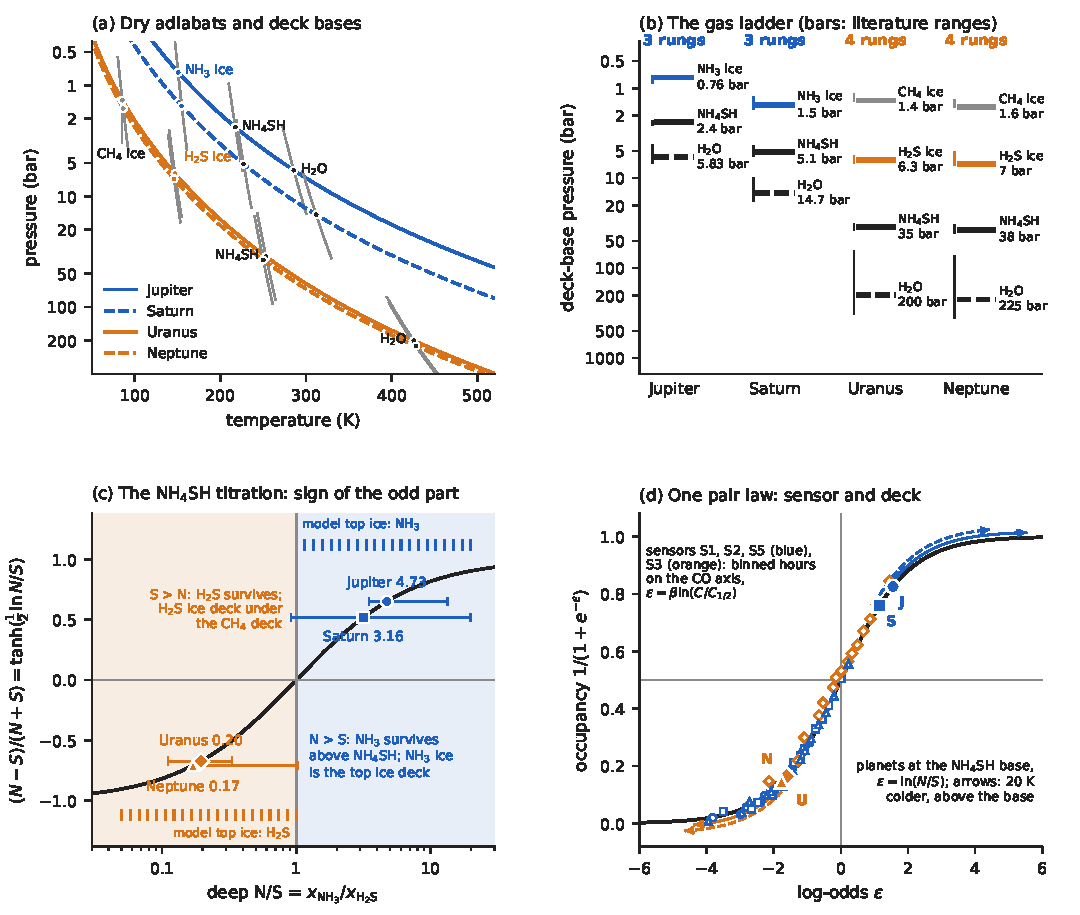
\includegraphics[width=\textwidth]{fig_gas_ladder.pdf}
\caption{The gas ladder of the four giants from the equilibrium cloud-condensation model: dry adiabat of normal H$_2$ with He and CH$_4$, anchored at the NSSDC $1$-bar temperatures ($165$, $134$, $76$, $72$ K). Blue: deep $\mathrm N/\mathrm S>1$ (Jupiter solid, Saturn dashed); orange: $\mathrm N/\mathrm S<1$ (Uranus solid, Neptune dashed). (a) Pressure--temperature profiles with each deck's condensation curve (grey, for the planet's nominal abundances) and its base (dots, labelled for Jupiter and Uranus). (b) The ladder of deck bases: horizontal bars are the nominal bases, vertical bars span the bases over the literature abundance ranges ($179$ model cases); the rung count is shown at the top, $3,3,4,4$. (c) The NH$_4$SH titration: the signed survivor fraction $(\mathrm N-\mathrm S)/(\mathrm N+\mathrm S)=\tanh(\frac12\ln\mathrm N/\mathrm S)$ against deep N/S, zero at $\mathrm N/\mathrm S=1$, with the planets at their nominal N/S and literature ranges. Tick rows: the model's top ice deck across the N/S scan on the Uranus profile, identical on all four profiles. (d) One pair law, the logistic $1/(1+\e^{-\varepsilon})$. Open markers: binned hours of the metal-oxide sensors S1, S2, S5 (blue) and S3 (orange) of the chemistry companion \cite{SChem} on the CO axis, with $\varepsilon=\beta\ln(C/C_{1/2})$ and occupancy $(S-S_\mathrm{lo})/(S_\mathrm{hi}-S_\mathrm{lo})$. Filled markers: the four planets at their NH$_4$SH bases, where $\varepsilon=\ln(\mathrm N/\mathrm S)$ exactly; arrows follow $\varepsilon$ to $20$ K colder, above the base, towards $\mathrm{sign}(\mathrm N-\mathrm S)\cdot\infty$.}\label{fig:ladder}
\end{figure}

\section{The giants as a set}\label{sec:set}
\subsection{The classical order and the week}\label{sec:week}
Order the seven classical bodies by decreasing period: Saturn, Jupiter, Mars, Sun, Venus, Mercury, Moon (the Chaldean order). Give each hour of the day to the next body in this order, and name each day for the body of its first hour, as Cassius Dio describes \cite{Dio}. Consecutive days then advance by $24\bmod7=3$ places, which draws the star heptagram $\{7/3\}$ through the period order, and the days come out as Saturday, Sunday, Monday, Tuesday (Mars), Wednesday (Mercury), Thursday (Jupiter), Friday (Venus). The week is the period order of the bodies read in steps of three.

\subsection{Moon systems: a locked triad and a fourth, and pairs}\label{sec:moons}
The sidereal periods of the Galilean moons are Io $1.769138$, Europa $3.551181$, Ganymede $7.154553$ and Callisto $16.689017$ days \cite{NSSDCJsat}, so their mean motions are $203.488931$, $101.374726$, $50.317609$ and $21.571073$ deg/day. The inner three form two pairs, each near $2{:}1$ (period ratios $2.00729$ and $2.01470$), and the two pairs are tied to each other:
\[
n_\mathrm{Io}-2n_\mathrm{Eu}=0.739479,\qquad n_\mathrm{Eu}-2n_\mathrm{Ga}=0.739508\ \text{deg/day}.
\]
Their difference, the Laplace combination $n_\mathrm{Io}-3n_\mathrm{Eu}+2n_\mathrm{Ga}$, is $-0.000029$ deg/day, $1.4\times10^{-7}$ of Io's motion and below the $1.1\times10^{-4}$ deg/day allowed by the six-decimal rounding of the periods. The Io--Europa conjunctions recur every $3.5255$ days and the Europa--Ganymede conjunctions every $7.0509$ days, exactly twice as long. The three moons are one locked triad; the Laplace resonance holds its angle at $180^\circ$, so a triple conjunction never occurs. Callisto stands outside the lock, at a period ratio of $2.33264$ to Ganymede: Jupiter's large moons are a triad with a fourth body beside it (\cref{fig:jup}b). Saturn's moons \cite{NSSDCSsat} lock in pairs: Tethys/Mimas $=2.00314$ ($2{:}1$, $+0.157\%$), Dione/Enceladus $=1.99743$ ($2{:}1$, $-0.128\%$) and Hyperion/Titan $=1.33434$ ($4{:}3$, $+0.075\%$).

\subsection{Jupiter and Saturn meet at thirds of a turn}\label{sec:trigon}
The period ratio of Saturn to Jupiter is $P_S/P_J=10759.22/4332.589=2.48332$ \cite{NSSDCJ,NSSDCS}, close to $\frac52$. Their synodic period is $7253.45$ days, or $19.859$ years. In that time Jupiter moves $602.698^\circ$, so each conjunction falls $242.698^\circ=0.67416$ of a turn beyond the previous one; at an exact $5{:}2$ ratio the advance would be $\frac{5/2}{3/2}-1=\frac23$ of a turn. Three conjunctions therefore close a triangle, the trigon, which turns by $3\times242.698^\circ-720^\circ=8.095^\circ$ every $59.58$ years.

\begin{proposition}[the trigon and the great inequality]\label{prop:trigon}
Let $n_J$, $n_S$ be the mean motions in turns per unit time. Each corner of the trigon turns at the rate $\frac13(5n_S-2n_J)$, so the trigon advances one third of a turn in exactly one period $1/|2n_J-5n_S|$ of the great inequality.
\end{proposition}
\begin{proof}
Conjunctions recur every $S=1/(n_J-n_S)$. In that time Jupiter moves $n_JS$ turns, and the conjunction point advances $n_JS$ turns, which is $\frac53+\Delta$ with $\Delta=n_JS-\frac53$ the excess over the exact $5{:}2$ advance of $\frac23$ of a turn modulo $1$. Every third conjunction returns to the same corner, moved on by $3\Delta$ turns after $3S$. The corner's rate is $\Delta/S=n_J-\frac53(n_J-n_S)=\frac13(5n_S-2n_J)$, and $\frac13$ of a turn takes $1/|5n_S-2n_J|$.
\end{proof}
With the NSSDC periods the great inequality has period $883$ years, and $120^\circ/8.095^\circ\times59.58$ years $=883$ years. From the ephemeris we find the heliocentric conjunctions of 1802--2080 (\cref{fig:jup}a). Successive advances vary from $224^\circ$ to $255^\circ$ because both orbits are eccentric; their mean is $242.1^\circ$. Every third conjunction returns to the same corner, moved on by $8.6^\circ$ on average: $159^\circ$ (1802), $169^\circ$ (1861), $178^\circ$ (1921), $187^\circ$ (1981) and $196^\circ$ (2040); $25^\circ$ (1821) to $62^\circ$ (2060); and $280^\circ$ (1842) to $309^\circ$ (2080). The 2020 heliocentric conjunction, on 2 November at $301.5^\circ$, preceded the geocentric great conjunction of 21 December 2020 near $300.5^\circ$.

\begin{figure}[!htb]\centering
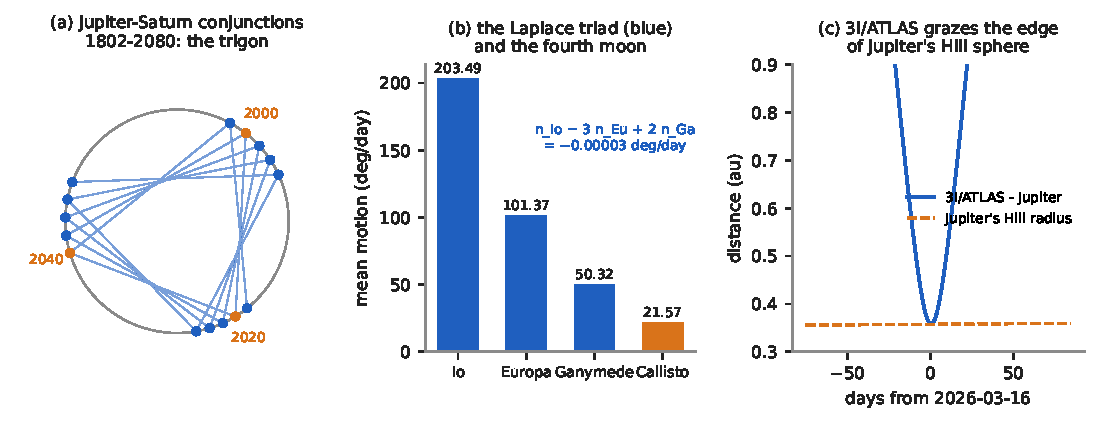
\includegraphics[width=\textwidth]{fig_jup.pdf}
\caption{(a) Heliocentric Jupiter--Saturn conjunctions 1802--2080, joined in time order; each falls about two thirds of a turn after the last; those of 2000, 2020 and 2040 in orange. (b) Mean motions of the Galilean moons: the Laplace triad (blue) and Callisto (orange). (c) The distance of 3I/ATLAS from Jupiter (blue) and Jupiter's Hill radius (orange), which meet at closest approach (\cref{sec:contact}).}\label{fig:jup}
\end{figure}

\subsection{The triangle is a triad with a centre}\label{sec:triangle}
The equilateral configuration of three masses rotates rigidly. Gascheau and Routh \cite{Gascheau,Routh,Sicardy} showed that it is linearly stable exactly when
\[
(m_1+m_2+m_3)^2>27(m_1m_2+m_2m_3+m_3m_1).
\]
The criterion forces a dominant centre: if $m_1$ is the largest mass and $M$ the total, then $\sum_{i<j}m_im_j\ge m_1(M-m_1)$, so $27\,x(1-x)<1$ with $x=m_1/M\ge\frac13$, hence $m_1>(1-\mu_G)M=0.9614791\,M$, where $\mu_G=\frac12(1-\sqrt{23/27})=0.0385209$ is Routh's critical value \cite{SPhys,MHO}. For a planet and a test body the criterion reads $27\mu(1-\mu)<1$, that is $\mu<\mu_G$. The computed spectra agree with the criterion for $2000$ values of $\mu$ and for $2000$ random mass triples spanning six decades ($870$ of them stable), with real parts below $1.05\times10^{-7}$ of the rotation rate on the stable side and above $1.34\times10^{-2}$ on the unstable side. Three equal masses are unstable, with growth rate $0.7071=1/\sqrt2$ of the rotation rate, the equal-mass Lagrange triangle of the physics companion \cite{SPhys}: a triangle stands only around a dominant centre.

\begin{proposition}[on the axis, and off it in mirrored fours]\label{prop:krein}
At $L_4$ of the restricted problem the characteristic polynomial is $\lambda^4+\lambda^2+\frac{27}4\mu(1-\mu)=0$. For $\mu<\mu_G$ its roots are two pairs $\pm i\omega_1$, $\pm i\omega_2$ on the imaginary axis with $\omega_1^2+\omega_2^2=1$ and $\omega_1^2\omega_2^2=\frac{27}4\mu(1-\mu)$; they meet at $\omega=1/\sqrt2$ exactly at $\mu=\mu_G$, and for $\mu>\mu_G$ they form the quadruple $\pm a\pm ib$ off the axis.
\end{proposition}
\begin{proof}
At $L_4$, $U_{xx}=\frac34$, $U_{yy}=\frac94$ and $U_{xy}=\frac{3\sqrt3}4(1-2\mu)$ \cite{MD}. The linearised equations $\ddot x-2\dot y=U_{xx}x+U_{xy}y$, $\ddot y+2\dot x=U_{xy}x+U_{yy}y$ give $\lambda^4+(4-U_{xx}-U_{yy})\lambda^2+U_{xx}U_{yy}-U_{xy}^2=0$, and $U_{xx}U_{yy}-U_{xy}^2=\frac{27}{16}[1-(1-2\mu)^2]=\frac{27}4\mu(1-\mu)$. Hence $\lambda^2=\frac12[-1\pm\sqrt{1-27\mu(1-\mu)}]$, both negative for $27\mu(1-\mu)<1$, equal to $-\frac12$ at equality, and complex conjugate beyond.
\end{proof}
The eigenvalues of a real linear Hamiltonian system come in fours, $\{\lambda,-\lambda,\bar\lambda,-\bar\lambda\}$: the spectrum is invariant under the Klein four-group $V$ generated by $\lambda\mapsto-\lambda$ (the Hamiltonian symmetry) and $\lambda\mapsto\bar\lambda$ (reality). On the fixed line of $\lambda\mapsto-\bar\lambda$, the imaginary axis, an orbit of $V$ collapses to a pair $\{\lambda,-\lambda\}$. The Krein signature of a pair on the axis is the sign of the quadratic Hamiltonian on its eigenspace, the sign of the mode's energy. Krein's theorem states that under a continuous Hamiltonian perturbation a pair of definite signature stays on the axis until it collides with a pair of opposite signature (or at zero) \cite{MHO}. Below $\mu_G$ the two pairs at $L_4$ have opposite signatures on all $155$ grid values: the slow libration carries negative energy (at $\mu=10^{-6}$, $\omega=0.002598$, signature $-1$) and the fast epicycle positive ($\omega=0.999997$, $+1$). They meet at $1/\sqrt2$ at $\mu_G$, and at $\mu_G(1+10^{-4})$ the four are $\pm0.00346\pm0.70712\,i$ (\cref{fig:throats}b). With $\lambda=s-\frac12$ the zeros of Riemann's $\xi$ are invariant under the same group: $\xi(s)=\xi(1-s)$ is $\lambda\mapsto-\lambda$ and $\xi(\bar s)=\overline{\xi(s)}$ is $\lambda\mapsto\bar\lambda$; the fixed line of $\lambda\mapsto-\bar\lambda$ is the critical line, and the Riemann Hypothesis states that every orbit of $V$ on the zero set is a pair on that line \cite{SMath}. The Lee--Yang zeros of a real partition function that is symmetric under reversal of the field carry the same group in the variable $\lambda=\frac12\ln z$: $z\mapsto1/z$ is $\lambda\mapsto-\lambda$, $z\mapsto\bar z$ is $\lambda\mapsto\bar\lambda$, and the fixed line is the unit circle; there positive coupling keeps every zero on the circle, and a negative coupling sends zeros off it in mirrored pairs $z,1/\bar z$ \cite{SQuant}. In all three settings one mechanism holds. A simple zero $iy\ne0$ on the fixed line is an orbit of two, $\{iy,-iy\}$, and under a small perturbation that respects $V$ it stays on the line: off the line its orbit would put two zeros ($\lambda$ and $-\bar\lambda$) near $iy$, where the perturbed function has only one. Zeros leave the line only where two of them meet, and away from $\lambda=0$ they leave as a quadruple $\{\lambda,-\lambda,\bar\lambda,-\bar\lambda\}$. Krein's theorem sharpens this for Hamiltonian spectra: a meeting sends two pairs off the axis only if their signatures are opposite. Below $\mu_G$ the two frequencies stand in the ratio $2{:}1$ at $\mu=0.0242939$ and $3{:}1$ at $\mu=0.0135160$, both inside the linearly stable range.

\paragraph{Trojans at all four.} All four giants satisfy the criterion (the largest $27\mu(1-\mu)$ is Jupiter's, $2.57\times10^{-2}$), and Trojans are now known at all four: Jupiter's long-known clouds; Neptune's $35$ by the 2023 count, $28$ at $L_4$ and $7$ at $L_5$ \cite{WikiMoons}; Uranus's two transient ones, 2011~QF$_{99}$ and 2014~YX$_{49}$ \cite{dlFM}; and Saturn's one, 2019~UO$_{14}$, confirmed in 2024, captured about $2000$ years ago and leaving in about $1000$ \cite{HuiTrojan}. For primordial Trojans in the present planetary configuration, Nesvorn\'y and Dones found Saturn's and Uranus's depleted about $100$-fold over the age of the Solar System, while Neptune may retain about half \cite{NesvornyDones}. Since the three-body triangles are linearly stable, the depletion comes from the rest of the planetary system, which is to each triangle a fourth body. The libration periods at $L_4$ are $P_\mathrm{orb}/\omega_\mathrm{slow}$, $147.4$, $670.2$, $4893$ and $8837$ years for the four giants (\cref{tab:throats}).

\subsection{Four is three and a zero}\label{sec:zeromode}
To first order in the masses the inclinations of the four orbits evolve under the Laplace--Lagrange equations $\dot{\mathbf p}=B\mathbf q$, $\dot{\mathbf q}=-B\mathbf p$, with $p_j=I_j\sin\Omega_j$, $q_j=I_j\cos\Omega_j$ and the $4\times4$ matrix
\[
B_{jk}=\frac{n_j}4\,\frac{m_k}{M_\odot+m_j}\,\alpha_{jk}\bar\alpha_{jk}\,b^{(1)}_{3/2}(\alpha_{jk})\ (j\ne k),\qquad B_{jj}=-\sum_{k\ne j}B_{jk},
\]
where $b^{(1)}_{3/2}$ is a Laplace coefficient \cite{MD}.
\begin{proposition}[the zero mode]\label{prop:zeromode}
$B$ has the eigenvalue $0$ with eigenvector $(1,1,1,1)$: a common tilt of all four orbits, which is a rotation of the reference plane, does not evolve. Its invariant plane is the invariable plane, perpendicular to the total orbital angular momentum.
\end{proposition}
\begin{proof}
Every row of $B$ sums to zero by construction. A common tilt changes all $(p_j,q_j)$ by the same vector, which the equations leave fixed; the plane so defined is fixed by the conserved total angular momentum.
\end{proof}
With the NSSDC masses and semimajor axes and the Laplace coefficients by quadrature, the eigenvalues of $B$ are $-25.5183$, $-2.9276$, $-0.6698$ and $0$ arcsec/yr, the zero to $6\times10^{-17}$ of the largest. The three live modes have periods of $50{,}787$, $442{,}677$ and $1{,}935{,}044$ years. The zero mode is occupied by no body; it is fixed by the total angular momentum, of which Jupiter carries $0.6158$, Saturn $0.2501$, Neptune $0.0800$ and Uranus $0.0541$. The eccentricities have four live modes, $0.6254$, $2.7168$, $3.6869$ and $22.0865$ arcsec/yr, and no zero.

\subsection{No barrier between the four}\label{sec:chain}
\begin{proposition}[tangent orbits lie below the throats]\label{prop:tisserand}
An orbit coplanar with two circular planetary orbits, with perihelion on the inner and aphelion on the outer, has Tisserand parameter $\mathcal T=1-e+2\sqrt{1+e}$ with respect to the inner planet and $\mathcal T=1+e+2\sqrt{1-e}$ with respect to the outer, and both are below $3$ for every $e>0$.
\end{proposition}
\begin{proof}
With respect to a planet at $a_p$, $\mathcal T=a_p/a+2\sqrt{(a/a_p)(1-e^2)}$. Perihelion at $a_p$ means $a=a_p/(1-e)$, which gives $\mathcal T=1-e+2\sqrt{1+e}$; aphelion at $a_p$ means $a=a_p/(1+e)$, which gives $1+e+2\sqrt{1-e}$. Both equal $3$ at $e=0$ and have derivatives $-1+(1+e)^{-1/2}<0$ and $1-(1-e)^{-1/2}<0$.
\end{proof}
Since $\mathcal T\approx C$ for a small body and $C(L_1),C(L_2)>3$ (\cref{tab:throats}), every tangent orbit is energetically open to both throats of both planets. For Jupiter--Saturn, Saturn--Uranus and Uranus--Neptune, $\mathcal T=2.981/2.974$, $2.976/2.966$ and $2.989/2.986$, below even $C(L_4)$: at these energies the zero-velocity surfaces place no barrier between the four realms. The tangent orbits take $10.04$, $27.23$ and $61.28$ years per hop, and one tangent orbit from Jupiter to Neptune takes $37.21$ years; the arches of chaos do it in under a decade \cite{Todorovic}.

\subsection{Two thirds of the horizon is filled at three giants}\label{sec:reach}
The Hill radius $r_H=a(m/3M_\odot)^{1/3}$ bounds each giant's family of moons. We read the moon tables: all $29$ moons of Uranus and $16$ of Neptune; for Saturn the $210$ Norse-group moons with eccentricities and $35$ Gallic and Inuit moons with semimajor axes only; for Jupiter $13$ outer moons with eccentricities and $21$ with semimajor axes only \cite{WikiMoons}. Every listed moon lies inside its Hill sphere.

The largest apocentres $a(1+e)$, in units of $r_H$, are $0.6326$ for Jupiter (S/2017~J~14), $0.6255$ for Saturn (S/2023~S~5), $0.4070$ for Uranus (Ferdinand) and $0.6543$ for Neptune (S/2021~N~1; Neso $0.6233$) (\cref{fig:throats}c). Three of the four lie within $10\%$ of two thirds, in $0.600$--$0.733\,r_H$, with mean $0.6374$. Nine of Jupiter's twelve largest orbits are listed without eccentricities; those moons would carry the reach beyond $0.733\,r_H$ only with $e>0.638$, and Saturn's only with $e>1$. The reach agrees with the known dynamics of irregular satellites: planar retrograde orbits are long-lived to $a\approx0.7\,r_H$, prograde ones only to $0.4\,r_H$ \cite{Nesvorny03}, and the moons with the largest apocentres at all four giants are retrograde.

\paragraph{The exception, and a prediction.} Uranus's moons stop at $0.41$ of its Hill radius; its retrograde moon with the largest apocentre has $a/r_H=0.29$, against $0.44$, $0.39$ and $0.44$ for the other three giants. We predict that Uranus has undiscovered retrograde irregular moons with apocentres of $0.60$--$0.73\,r_H$, $42$--$51$ million km from the planet.

\section{The visitors}\label{sec:visitors}
\subsection{Three interstellar objects on every measured axis}\label{sec:iso}
We compare the three known interstellar objects on every axis with published measurements. Orbital elements are JPL solutions: 1I from the Small-Body Database (solution 16) \cite{JPL1I}, 2I and 3I as quoted from JPL in \cite{W2I,W3I}. The other quantities come from the sources cited in each table; where studies disagree we quote the range. Directions, deflections, velocities relative to the local standard of rest (LSR) and traceback separations are computed from these inputs, with the solar motion $(U,V,W)_\odot=(11.1,12.24,7.25)$ km/s \cite{SBD10}.

\begin{table}[!htb]\centering\small\setlength{\tabcolsep}{4pt}
\begin{tabular}{@{}>{\raggedright\arraybackslash}p{2.9cm}>{\raggedright\arraybackslash}p{3.7cm}>{\raggedright\arraybackslash}p{3.7cm}>{\raggedright\arraybackslash}p{4.1cm}@{}}\toprule
 & 1I/\textquoteleft Oumuamua & 2I/Borisov & 3I/ATLAS\\\midrule
designation & A/2017 U1 & C/2019 Q4 & C/2025 N1\\
perihelion (TDB) & 2017 Sep 9.51 & 2019 Dec 8.56 & 2025 Oct 29.51\\
$q_\mathrm{p}$ (au) & $0.25591$ & $2.0065$ & $1.3564$\\
$e$ & $1.20113$ & $3.3565$ & $6.1414$\\
$i$ & $122.74^\circ$ & $44.05^\circ$ & $175.12^\circ$\\
$v_\infty$ (km/s) & $26.32$ & $32.28$ & $57.94$\\
incoming RA, Dec & $279.55^\circ$, $+33.90^\circ$ (Lyra) & $32.81^\circ$, $+59.46^\circ$ (Cassiopeia) & $295.05^\circ$, $-19.07^\circ$ (Sagittarius)\\
outgoing RA, Dec & $357.83^\circ$, $+24.70^\circ$ & $275.44^\circ$, $-51.99^\circ$ & $95.18^\circ$, $+19.76^\circ$\\
deflection $2\arcsin(1/e)$ & $112.7^\circ$ & $34.7^\circ$ & $18.7^\circ$\\\bottomrule
\end{tabular}
\caption{Direction and orbit. $q_\mathrm{p}$ is the perihelion distance. The incoming directions of 1I and 3I agree with the published radiants to $0.1^\circ$ \cite{ISSI19,dlFM25}; that of 2I is computed from its elements. $v_\infty$ from \cite{Mamajek17,Hui20,dlFM25}.}\label{tab:isodir}
\end{table}

\paragraph{Direction.} We asked whether the three incoming directions share a common point: whether they cluster (circumradius), lie on one great circle ($|\det[\mathbf r_1\mathbf r_2\mathbf r_3]|$), have orbit planes that share one line ($|\det|$ of the poles), or have a circumcentre near the solar apex, the Galactic Centre, the anticentre or the Galactic pole. Each statistic was compared with an isotropic population and a kinematic population ($10^6$ draws each). The kinematic population draws stellar velocities from a Gaussian ellipsoid with dispersions $(35,25,18)$ km/s about the LSR, weighted by the encounter rate $v(1+(42.1\ \mathrm{km/s}/v)^2)$ with gravitational focusing at $1$ au. The three directions share no point: none of the eight statistics departs from either population. The circumradius, $57.2^\circ$, lies below the population medians $69.6^\circ$ and $66.1^\circ$ with $p=0.27$ (isotropic) and $0.35$ (kinematic); the great circle gives $p=0.73/0.78$, the common orbital line $0.76/0.77$ and the reference points $0.87/0.89$ (with the antipode rule the Galactic Centre and anticentre are one statistic); and the smallest enclosing circle, of radius $55.1^\circ$, gives $p=0.32$. The directions carry known physics instead: 1I came from $15^\circ$ from the solar apex, as expected for a slow object, and 3I from $28^\circ$ from the Galactic Centre.

\begin{table}[!htb]\centering\small\setlength{\tabcolsep}{4pt}
\begin{tabular}{@{}>{\raggedright\arraybackslash}p{2.6cm}>{\raggedright\arraybackslash}p{3.8cm}>{\raggedright\arraybackslash}p{3.9cm}>{\raggedright\arraybackslash}p{4.2cm}@{}}\toprule
 & 1I & 2I & 3I\\\midrule
heliocentric $(U,V,W)$ (km/s) & $(-11.46,-22.40,-7.75)$ \cite{Mamajek17} & $(22.0,-23.6,1.1)$ \cite{TS25} & $(-51.23,-19.46,18.93)$ \cite{dlFM25}\\
relative to LSR (km/s) & $(-0.4,-10.2,-0.5)$; $10.2$ & $(33.1,-11.4,8.4)$; $36.0$ & $(-40.1,-7.2,26.2)$; $48.5$\\
$z_{\max}$ (kpc) \cite{KL26} & $0.016$ & $0.121$ & $0.481$\\
kinematic age (Gyr) \cite{TS25} & $1.2^{+4.3}_{-1.0}$ & $4.8^{+4.7}_{-2.8}$ & $6.9^{+4.1}_{-3.3}$\\
population & young thin disk; no parent \cite{Mamajek17} & thin disk; Ross~573 fly-by, not a parent \cite{BJ20} & thick-disk-like, metal-poor host favoured \cite{Hopkins25,KL26}\\\bottomrule
\end{tabular}
\caption{Origin and kinematics.}\label{tab:isokin}
\end{table}

\paragraph{Origin.} Members of one star, cluster or moving group differ in velocity by a few km/s. The three objects differ by up to $75.5$ km/s relative to the LSR ($34.6$ for 1I--2I, $48.0$ for 1I--3I, $75.5$ for 2I--3I). Triples drawn from the kinematic population give a median largest difference of $75.4$ km/s ($p=0.50$), and a difference below $10$ km/s occurs in $5\times10^{-5}$ of them. On straight-line paths the three were $35$--$77$ pc apart one million years ago and $354$--$772$ pc apart ten million years ago, so they share no recent point of release: the three interstellar objects share neither a direction nor a kinematic origin. Speed ($26\to32\to58$ km/s), kinematic age ($1\to5\to7$ Gyr) and vertical excursion ($0.016\to0.12\to0.48$ kpc) rise together; the ages and excursions are inferred from the velocities, so this is one fact, the age--velocity relation of the Galactic disk, by which faster objects are assigned to older, dynamically hotter parts of the disk \cite{Hopkins25,TS25}.

\begin{table}[!htb]\centering\small\setlength{\tabcolsep}{4pt}
\begin{tabular}{@{}>{\raggedright\arraybackslash}p{2.3cm}>{\raggedright\arraybackslash}p{4.2cm}>{\raggedright\arraybackslash}p{4.2cm}>{\raggedright\arraybackslash}p{4.2cm}@{}}\toprule
 & 1I & 2I & 3I\\\midrule
discovery & 2017 Oct 19, Pan-STARRS1, Haleakal\=a \cite{Meech17} & 2019 Aug 30, G.~Borisov, Crimea \cite{MPEC19} & 2025 Jul 1, ATLAS Chile \cite{MPEC25}\\
relative to perihelion & $40$ d after & $100$ d before & $120$ d before (TESS images from May \cite{Feinstein25})\\\bottomrule
\end{tabular}
\caption{Time.}\label{tab:isotime}
\end{table}

\paragraph{Time.} Each object was found within about four months of perihelion, when it was brightest and nearest.

\begin{table}[!htb]\centering\small\setlength{\tabcolsep}{4pt}
\begin{tabular}{@{}>{\raggedright\arraybackslash}p{2.4cm}>{\raggedright\arraybackslash}p{3.7cm}>{\raggedright\arraybackslash}p{3.7cm}>{\raggedright\arraybackslash}p{4.5cm}@{}}\toprule
 & 1I & 2I & 3I\\\midrule
absolute magnitude & $H_V=22.4\pm0.04$ \cite{ISSI19} & nucleus hidden by coma & nucleus $H_V=17.1\pm0.4$ \cite{Hui26}\\
radius & $\sim0.1$ km (albedo $0.04$) \cite{Meech17}; Spitzer: $<49$--$220$ m \cite{Trilling18} & $0.2$--$0.5$ km \cite{Jewitt20} & $1.3\pm0.2$ km \cite{Hui26}; $0.4$--$1.2$ km from non-grav.\ \cite{Thoss26}\\
slope (\%/100 nm) & $9$--$23$ (studies differ) \cite{ISSI19} & $10.6\pm1.4$ \cite{Hui20} & $17.1\pm0.2$ \cite{Seligman25}; $18.3\pm0.9$ \cite{dlFM25}\\
class & D-type-like & like Solar System comets & slightly redder than D-type; TNO/Centaur-like\\
polarisation & not measured & high positive, like Hale--Bopp \cite{Bagnulo21} & deep negative branch, $-2.7\%$ at $7^\circ$, inversion $17^\circ$ \cite{Gray25}\\\bottomrule
\end{tabular}
\caption{Brightness, size, colour and polarisation.}\label{tab:isophot}
\end{table}

\paragraph{Brightness, colour, rotation.} All three are moderately red and none is ultrared; nucleus sizes span roughly a factor of ten, with large uncertainties for the two active objects (\cref{tab:isophot}). 3I's negative polarisation branch is unprecedented \cite{Gray25}. 1I rotated in $8.67\pm0.34$ h \cite{ISSI19} or $8.1$ h \cite{Bolin18}, tumbling, with a lightcurve amplitude of $1.5$--$2.5$ mag and axis ratio at least $6{:}1$; 2I has no secure period; 3I rotates in $16.16\pm0.01$ h \cite{SantanaRos25} or $16.79\pm0.23$ h \cite{dlFM25}, with amplitude $0.2$--$0.3$ mag; the Hubble Space Telescope images were too sparsely sampled to fix a period \cite{Hui26}. The ratio $16.16/8.1=1.995$ lies within $0.3\%$ of $2$, the factor by which lightcurve periods are commonly ambiguous. The free-floating planetary-mass object PSO~J318.5$-$22 rotates in $8.6\pm0.1$ h \cite{Biller18} and lies $22^\circ$ from the direction 3I came from, and $68^\circ$ and $102^\circ$ from those of 1I and 2I.

\begin{table}[!htb]\centering\footnotesize\setlength{\tabcolsep}{3.5pt}
\begin{tabular}{@{}>{\raggedright\arraybackslash}p{2.0cm}>{\raggedright\arraybackslash}p{2.8cm}>{\raggedright\arraybackslash}p{3.6cm}>{\raggedright\arraybackslash}p{3.8cm}>{\raggedright\arraybackslash}p{2.3cm}@{}}\toprule
species & 1I & 2I & 3I & Solar System comets\\\midrule
activity & none; dust $<1.7\times10^{-3}$ kg/s \cite{ISSI19} & coma at discovery; active by $7.8$ au \cite{Ye20} & coma at discovery; CN from $\approx3$ au \cite{Rahat25} & --\\
CO (CO/H$_2$O) & rate $<9\times10^{23}$ s$^{-1}$, no H$_2$O seen \cite{Trilling18} & $0.35$--$1.05$ \cite{Cordiner20}; $\ge1.7$ \cite{Bodewits20} & $1.65\pm0.09$ at $3.32$ au \cite{Cordiner25} & median $0.03$ \cite{HP22}\\
CO$_2$ (CO$_2$/H$_2$O) & rate $<9\times10^{22}$ s$^{-1}$ \cite{Trilling18} & not measured & $7.6\pm0.3$ at $3.32$ au \cite{Cordiner25}; $0.3$--$2.1$ after perihelion \cite{Shinnaka26} & median $0.12$ \cite{HP22}\\
C$_2$ & -- & depleted (C$_2$/CN $0.1$--$0.3$) \cite{Deam26} & strongly depleted \cite{Paek26} & mostly not depleted\\
nickel, iron & -- & Ni and Fe; $\log(\mathrm{Ni/Fe})=0.21\pm0.18$ \cite{GD21,Opitom21} & Ni without Fe before $2.64$ au \cite{Rahat25}; $\log(\mathrm{Ni/Fe})\approx0.9\to0.3$ \cite{Hutsemekers26} & $-0.06\pm0.31$ \cite{Manfroid21}\\
isotopes & -- & -- & $^{12}$C/$^{13}$C $\approx151$, $^{14}$N/$^{15}$N $\approx363$, large errors \cite{Opitom26} & $\approx90$, $\approx150$ \cite{Opitom26}\\\bottomrule
\end{tabular}
\caption{Activity and composition.}\label{tab:isocomp}
\end{table}

\paragraph{Activity, composition and acceleration.} 2I and 3I share comae rich in carbon oxides relative to water (carbon monoxide for 2I, carbon dioxide and monoxide for 3I), far above Solar System medians; depleted C$_2$; and gas-phase nickel (\cref{tab:isocomp}). These point to formation or storage at low temperature, far from their stars. Nickel near $2$ au is also seen in Solar System comets \cite{Manfroid21}; what is distinctive in 3I is nickel (Ni\,\textsc{i} \cite{Rahat25}) \emph{before} iron, with $\log(\mathrm{Ni/Fe})$ falling from $\approx0.9$ towards Solar System values as it approached the Sun, which indicates a nickel carrier that releases at lower temperature \cite{Hutsemekers26}. 1I showed no gas or dust at deep limits, so its composition is unmeasured, and the proposed drivers of its acceleration (hydrogen from irradiated water ice, a nitrogen-ice fragment, radiation pressure on a thin body) remain to be decided \cite{BS23,JD21}. All three show non-gravitational acceleration: the radial parameter at $1$ au is $(4.92\pm0.16)\times10^{-6}$ m\,s$^{-2}$ for 1I \cite{Micheli18}, $\approx5\times10^{-8}$ m\,s$^{-2}$ for 2I \cite{Hui20} and $\approx1\times10^{-6}$ m\,s$^{-2}$ for 3I \cite{Spada26}; the distance scalings differ, so the ordering is approximate. For 2I and 3I the acceleration matches their measured outgassing \cite{Hui20,Thoss26}; for 1I no outgassing was seen.

\begin{table}[!htb]\centering\small
\begin{tabular}{@{}>{\raggedright\arraybackslash}p{2.6cm}>{\raggedright\arraybackslash}p{5.4cm}>{\raggedright\arraybackslash}p{6.0cm}@{}}\toprule
axis & shared & not shared\\\midrule
direction & -- (no common point) & Lyra, Cassiopeia, Sagittarius; spread typical of random directions\\
origin, time & Galactic disk & separate sources; inferred ages $1$, $5$, $7$ Gyr\\
dates & found near perihelion (selection) & discovered in 2017, 2019 and 2025\\
size, brightness & small bodies & factor $\sim10$ in radius\\
colour & moderately red, not ultrared & 3I redder than 2I\\
polarisation & -- & 2I strongly positive; 3I deeply negative\\
rotation & -- & 1I tumbling, very elongated; 3I small amplitude (diluted by coma)\\
activity & 2I and 3I active & 1I inert\\
composition & 2I and 3I: carbon-oxide-rich, C$_2$-depleted, nickel & 3I: nickel before iron, CO$_2$-dominated\\
dynamics & non-gravitational acceleration in all three & strength and cause differ\\\bottomrule
\end{tabular}
\caption{Synthesis: kin, not siblings.}\label{tab:isosyn}
\end{table}

\paragraph{Kin, not siblings.} The answer on every axis is the same (\cref{tab:isosyn}). The three are samples of one population, the small bodies ejected from planetary systems throughout the Galactic disk, not three pieces of one source. They share what that population shares: they are red and small, and the two whose gas could be measured are rich in carbon oxides and carry nickel. They share no star, direction or date. What all three orbits have in common is the Sun as their focus, placed there by detection: interstellar objects are seen only when they pass close to us.

\subsection{At the giants: 3I/ATLAS touched Jupiter's Hill sphere}\label{sec:contact}
We propagated each object on its two-body hyperbola and found its closest approach to Mars, Jupiter and Saturn within ten years of perihelion (\cref{tab:isoplanets}). As validation, our 3I--Jupiter approach is $0.358011$ au at 2026-03-16 11:33 UT, against JPL's $0.358330$ au at 12:22 UT \cite{W3I}; our 3I--Mars approach is $0.1936$ au on 2025-10-03 and our 3I--Earth approach $1.798$ au on 2025-12-19, both matching the published values.

\begin{table}[!htb]\centering\small
\begin{tabular}{@{}llrrr@{}}\toprule
object & planet & closest (au), date & $r_H$ (au) & $d/r_H$\\\midrule
1I & Jupiter & $4.8069$, 2017-07-30 & $0.3720$ & $12.9$\\
1I & Saturn & $8.1799$, 2017-01-15 & $0.4599$ & $17.8$\\
2I & Jupiter & $5.1385$, 2020-05-25 & $0.3533$ & $14.5$\\
2I & Saturn & $8.8901$, 2020-10-27 & $0.4574$ & $19.4$\\
3I & Mars & $0.1936$, 2025-10-03 & $0.0073$ & $26.4$\\
3I & \textbf{Jupiter} & $\mathbf{0.3580}$, \textbf{2026-03-16} & $\mathbf{0.3576}$ & $\mathbf{1.001}$\\
3I & Saturn & $9.9791$, 2025-05-28 & $0.4389$ & $22.7$\\\bottomrule
\end{tabular}
\caption{Closest approaches and the planet's Hill radius $r_H=r(m/3M_\odot)^{1/3}$ at its distance $r$ from the Sun at that moment. 1I and 2I passed Mars at $190$ and $225$ Hill radii.}\label{tab:isoplanets}
\end{table}

\paragraph{The horizon touched.} Of the three interstellar objects, only 3I came near a giant planet. At its closest approach Jupiter was $5.238$ au from the Sun, and its Hill radius, the distance of $L_1$ and $L_2$ where Jupiter's gravity balances the Sun's tidal pull, was $0.3576$ au. 3I's closest approach was $0.3580$ au by our computation and $0.358330$ au by JPL: $1.0011$ and $1.0020$ Hill radii. With the Hill radius at Jupiter's mean distance ($0.3552$ au) the ratio is $1.008$. The object that arrived from $28^\circ$ from the Galactic Centre touched the balance sphere of the Sun--Jupiter pair and left (\cref{fig:jup}c). The approach was noted in advance by Loeb, Hibberd and Crowl, who showed that Juno could have been sent to within about $27$ million km of the object \cite{LoebJuno}.

\paragraph{The contact point.}
\begin{itemize}
\item \emph{When and how far:} 2026-03-16 11:33 UT (JPL: 12:22 UT), $53.56$ million km from Jupiter, passing at $65.90$ km/s relative to it.
\item \emph{Where in the Solar System} (heliocentric ecliptic J2000): $(-1.96319,\ +4.70277,\ -0.21433)$ au; longitude $112.658^\circ$, latitude $-2.408^\circ$, $5.1006$ au from the Sun.
\item \emph{Where in Earth's sky:} RA $06^\mathrm{h}50.6^\mathrm{m}$, Dec $+20.32^\circ$, in Gemini, $4.731$ au away and $4.14^\circ$ from Jupiter (RA $07^\mathrm{h}04.3^\mathrm{m}$, Dec $+22.98^\circ$); Galactic longitude $194.60^\circ$, latitude $+8.93^\circ$, $17.1^\circ$ from the Galactic anticentre. The object that arrived from near the Galactic Centre met Jupiter's sphere, as seen from Earth, near the opposite point of the sky.
\item \emph{Where on Jupiter's sphere:} $114^\circ$ from the anti-Sun direction and $66^\circ$ from the Sun direction, $42^\circ$ below Jupiter's orbital plane.
\item \emph{Relation to the throats:} the contact distance lies between Jupiter's $L_1$ distance ($0.3493$ au, sunward) and its $L_2$ distance ($0.3655$ au, anti-sunward), on the shell where the Sun--Jupiter balance sits; the point is $0.38$ au from $L_1$ itself and $0.61$ au from $L_2$.
\end{itemize}
3I's Jacobi constant was $C=-22.5$, against $3.0388$ at $L_1$ and $3.0375$ at $L_2$: far below the throat energies, so the zero-velocity surfaces placed no constraint on its path. It crossed the surface of the Sun--Jupiter balance sphere at speed, where the slow bodies of \cref{sec:topology} enter and leave only through the throats.

\paragraph{The configuration at the contact.} At the contact Jupiter led Saturn by $111.049^\circ$ in heliocentric longitude; in three dimensions the angle is $111.044^\circ$ (latitudes $+0.332^\circ$ and $-2.344^\circ$). The angle was growing by $0.0481^\circ$ per day and passed two exact values within months of the contact (\cref{fig:heart}d): $\arccos(-\frac13)=109.4712^\circ$, the angle whose cosine is minus one third, on 2026-02-11 ($32.6$ days before), and $120^\circ$, one third of a turn, on 2026-09-23; an ephemeris error of $0.05^\circ$ moves these dates by $1.0$ day. The value $111.049^\circ$ recurs twice per synodic cycle, with Jupiter and Saturn leading in turn: 2007-07-20, 2014-07-12, 2026-03-16, 2034-08-22. At the contact Saturn stood $8.00^\circ$ from the Sun in Earth's sky, and its conjunction with the Sun followed on 2026-03-25, $8.8$ days later. Three further angles of the configuration at the contact were Saturn--Sun--3I $108.474^\circ$, Sun--Earth--Jupiter $109.235^\circ$ and Sun--3I--Jupiter $110.658^\circ$. Around Saturn the sequence ran: equinox on 6 May 2025 \cite{AAQ}; 3I's closest approach to Saturn, $9.9791$ au, on 2025-05-28, $22.5$ days later; 3I's discovery on 1 July 2025; the southern decagon complete in August--September 2025; the contact on 16 March 2026. A body of $10$ km radius and density $1000$ kg/m$^3$ at $9.9791$ au pulls on Saturn with $1.25\times10^{-19}$ m/s$^2$, $1.3\times10^{-12}$ of the accelerations in Cassini's residuals: the sequence is one of timing, and the signal in Cassini's tracking is Saturn's own.

\paragraph{X-rays of 3I.} XRISM observed 3I for $17$ hours on 26--28 November 2025 and found carbon, nitrogen and oxygen lines from solar-wind charge exchange extending about $400\,000$ km from the nucleus; XMM-Newton also saw the diffuse glow \cite{ESAXRISM}.

\subsection{Radio: the Wow!\ signal, hydrogen and hydroxyl}\label{sec:radio}
The Wow!\ signal was recorded by the Big Ear telescope on 16 August 1977 at 03:16:06 UTC. The revised values are $1420.726\pm0.005$ MHz, at least $73.4$ s long, signal-to-noise ratio $30.1$, at least $256$ Jy, heliocentric radial velocity $-84\pm1$ km/s and LSR velocity $-74\pm2$ km/s; the two horn positions are RA $19^\mathrm{h}25^\mathrm{m}02^\mathrm{s}$ and $19^\mathrm{h}27^\mathrm{m}55^\mathrm{s}$ ($\pm3$ s), Dec $-26^\circ57'18''$ and $-26^\circ57'13''$ ($\pm20'$), and the beam is about $8'$ wide in right ascension \cite{Mendez25}. The printout's six characters \texttt{6EQUJ5} give the signal-to-noise ratio in successive $12$-s samples, $6$, $14$, $26$, $30$, $19$ and $5$ (lower edges) \cite{Ehman}. The proposed natural cause is a maser-like flare of a small cold hydrogen cloud \cite{Mendez24}.

\paragraph{Direction.} 3I came from RA $295.049^\circ$, Dec $-19.072^\circ$ (Galactic $l=20.73^\circ$, $b=-19.06^\circ$), $8.619^\circ$ from the positive-horn position and $8.371^\circ$ from the negative-horn position; 1I and 2I lie more than $61^\circ$ away (\cref{fig:sounds}a). Loeb noted that 3I arrived from near the direction of the Wow!\ signal \cite{LoebWow}. Its position and radial velocity in 1977 decide whether it could have been the source.

\paragraph{Position in 1977.} Propagated back to the Wow!\ epoch, 3I was $591.12$ au from the Sun, at RA $19^\mathrm{h}39^\mathrm{m}20.2^\mathrm{s}$, Dec $-19^\circ05'30''$ (J2000), $0.204^\circ$ from its incoming direction and $8.288^\circ$ from the nearer horn. The offsets are $+152.7'$ in RA (times $\cos$ Dec) and $+471.7'$ in Dec, against beam half-widths of $4'$ and $20'$.

\paragraph{Frequency.} In August 1977 3I moved at $58.013$ km/s, and its heliocentric radial velocity along the line of sight was $-58.012$ km/s, against the Wow!'s $-84\pm1$ km/s, a difference of $25.988$ km/s. Subtracting the observer's velocity along the line (Earth's orbital motion $-15.000$ km/s, its rotation $+0.026$ km/s at the Big Ear site) gives a topocentric velocity of $-43.038$ km/s. A transmitter on 3I at the hydrogen frequency would have been received at $1420.6097$ MHz, $116.3$ kHz below the Wow!, or $11.6$ of the receiver's $10$-kHz channels; to appear at $1420.726$ MHz it would have had to transmit at $1420.5221$ MHz. Our ephemeris converts the Wow!'s $1420.726$ MHz into $-84.47$ km/s heliocentric, against the published $-84\pm1$. The LSR radial velocities tell the same story: $-46.45$ km/s for 3I and $-74\pm2$ km/s for the Wow!. 3I/ATLAS was not the source of the Wow!\ signal: in 1977 it lay $8.3^\circ$ from the nearer beam centre, far outside a beam of half-widths $4'$ and $20'$, and a hydrogen-line transmitter on it would have been received $11.6$ channels from the Wow!.

\paragraph{Hydrogen: a triad and a fourth.} The Wow!\ lies $320.2$ kHz above the hydrogen line, $1420.405751768$ MHz \cite{Hellwig}, the flip between the two spin arrangements of hydrogen's electron and proton. The upper level, $F=1$, has three states, $m_F=-1,0,+1$; the lower level, $F=0$, has one. The line joins a triad to a single fourth state; the triad holds $\frac34$ of the degeneracy. This is the decomposition $\frac12\otimes\frac12=1\oplus0$ whose singlet is the fourth state of the physics and quantum companions \cite{SPhys,SQuant}.

\paragraph{Hydroxyl: two pairs about one centre.} 3I's radio lines are those of hydroxyl (OH). MeerKAT detected no OH on 20 and 28 September 2025, absorption at $1665$ and $1667$ MHz on 24 October and again on 4 and 6 November, and emission on 11--12 November \cite{UCT,AstroBio,ATel}. Searches for artificial signals found none: down to $0.17$ W over $900$--$1670$ MHz with MeerKAT \cite{UCT}, $10$--$110$ W over $1$--$9$ GHz with the Allen Telescope Array \cite{Sheikh}, and about $0.1$ W with the Green Bank Telescope \cite{BL}. OH's ground level is a pair of levels of opposite parity (the $\Lambda$-doublet), and each member splits into $F=1$ (three states) and $F=2$ (five). The four lines join the upper member to the lower \cite{Jiang}: $1612$ MHz is $F=1\to2$, $1720$ MHz is $F=2\to1$, $1665$ MHz is $F=1\to1$ and $1667$ MHz is $F=2\to2$. Writing $u_F$ and $\ell_F$ for the energies of the upper and lower members, $\nu_{1612}+\nu_{1720}=(u_1-\ell_2)+(u_2-\ell_1)$ and $\nu_{1665}+\nu_{1667}=(u_1-\ell_1)+(u_2-\ell_2)$ are the same combination of four level energies, so the two sums are equal. The measured frequencies satisfy this to the last digit:
\[
1612.2309+1720.5299=1665.4018+1667.3590=3332.7608\ \text{MHz}.
\]
Both pairs share one centre, $1666.38040$ MHz. The main lines sit at $\pm0.97860$ MHz from it and the satellites at $\pm54.14950$ MHz: two pairs $\pm s$ about one zero (\cref{fig:sounds}c). The hyperfine spacings are $55.1281$ MHz in the upper member and $53.1709$ MHz in the lower. The band between the hydrogen line and the OH lines is the ``water hole'', named by Bernard Oliver in 1971, where searches for other civilisations have long listened \cite{WaterHole}. The Wow!\ lies at its lower wall and 3I's OH lines at its upper wall; the span from $1420.405752$ to $1667.3590$ MHz is a ratio of $1.17386$, $2.775$ semitones.

\paragraph{3I's OH crossed its balance point.} The OH lines of a comet appear in absorption or emission against the sky according to the sign of the population difference between the two members of the doublet. That sign is set by sunlight: the Doppler shift of the comet against the Sun's absorption lines near $3086$\,\AA\ changes how strongly each level is pumped (the Swings effect \cite{Despois,Schleicher}, as used in \cite{Jiang}). Where the inversion passes through zero the two members are equally populated and the line vanishes. From our ephemeris, 3I's heliocentric radial velocity on the MeerKAT dates was $-45.12$ and $-40.13$ km/s on 20 and 28 September (no OH), $-8.452$ km/s on 24 October (absorption), $+10.139$ and $+13.373$ km/s on 4 and 6 November (absorption), and $+20.929$ and $+22.332$ km/s on 11 and 12 November (emission); the flip lies between $+13.37$ and $+20.93$ km/s. Comet C/2025 A6, observed by FAST in the same weeks while approaching the Sun, showed the opposite sequence \cite{Jiang}: emission at $-22.39$ and $-19.85$ km/s, absorption at $-9.34$, $-7.65$ and $-5.94$ km/s, and no detection closer to zero; its flip lies between $-19.85$ and $-9.34$ km/s (\cref{fig:sounds}d). Two comets, one on each side of zero velocity, crossed an inversion zero at speeds of similar size, as the Swings effect allows; they were at different distances from the Sun ($0.54$--$0.65$ au for C/2025 A6, $1.3687$--$1.4500$ au for 3I).

\subsection{The sounds of the giants and the visitors}\label{sec:sounds}
Each source has a sound it is known for and a vibration of its own body (\cref{tab:freq}). Jupiter's auroral electrons radiate by the cyclotron-maser process from a few kHz up to $40$ MHz, a limit set by a surface field of up to $14$ G \cite{Louis,SKAWB}; Saturn's kilometric radiation lies near $100$ kHz \cite{SKAWB}; 3I's OH line and rotation are as above, with a post-perihelion period of $7.136\pm0.001$ h \cite{ScarmatoLoeb}. As a terrestrial reference we include the periodical cicadas: \emph{Magicicada septendecim} sings a modulated pure tone sharply tuned at $1.3$ kHz, \emph{M.~cassini} in pulses with a broad peak near $6$ kHz \cite{YoungJosephson}, and a cicada's wings beat at $47\pm1$ Hz \cite{Wan}. Periodical cicadas emerge every $13$ or $17$ years, both prime, so a $13$-year and a $17$-year brood meet only every $\mathrm{lcm}(13,17)=221$ years; Broods XIX and XIII co-emerged in 2024 for the first time since 1803 and will next do so in 2245 \cite{BroodXIX}.

\begin{table}[!htb]\centering\small
\begin{tabular}{@{}lll@{}}\toprule
source & A: sound & B: vibration or spin\\\midrule
cicadas & song $1300$ Hz & wingbeat $47$ Hz\\
Jupiter & radio up to $40$ MHz & rotation $9.9250$ h\\
Saturn & kilometric radio $\sim100$ kHz & rotation $10^\mathrm{h}33^\mathrm{m}38^\mathrm{s}$\\
3I/ATLAS & OH $1667.3590$ MHz & rotation $16.16$ h\\
Wow! & $1420.726$ MHz & --\\\bottomrule
\end{tabular}
\caption{Characteristic frequencies of the sources: A, a sound each is known for; B, a vibration or spin of its body. \Cref{fig:sounds}b adds further characteristic frequencies of the same sources.}\label{tab:freq}
\end{table}

\paragraph{Sound mappings.} Each source is carried into hearing by whole octaves; the tones are synthesised from the published frequencies. The cicada song sounds at its own pitch, $1300$ Hz, and the wingbeat two octaves up at $188$ Hz. Jupiter's spin sounds at $117.389$ Hz ($22$ octaves up), its radio edge at $152.588$ Hz and its acoustic spacing at $162.844$ Hz. Saturn's interior spin sounds at $110.324$ Hz and beats against the hexagon's $109.332$ Hz at $0.9922$ Hz, and its kilometric radio at $195.312$ Hz. 3I's OH pair sounds at $794.125$ and $795.059$ Hz ($21$ octaves down), beating at $0.9333$ Hz, once every $1.072$ s, and its spin at $144.194$ Hz. The Wow!\ sounds at $677.455$ Hz, shaped by \texttt{6EQUJ5} with each $12$-s sample played as $1.2$ s, over the hydrogen line at $677.302$ Hz, with a beat every $6.549$ s. Jupiter's and Saturn's spin tones stand $1.075$ semitones apart. In each pair the beat is the difference of the two members: the OH beat is the main-line splitting $1.9572$ MHz divided by $2^{21}$, and the Wow!\ beat is its $320.2$ kHz offset from hydrogen divided by $2^{21}$.

\begin{figure}[!htb]
\centering
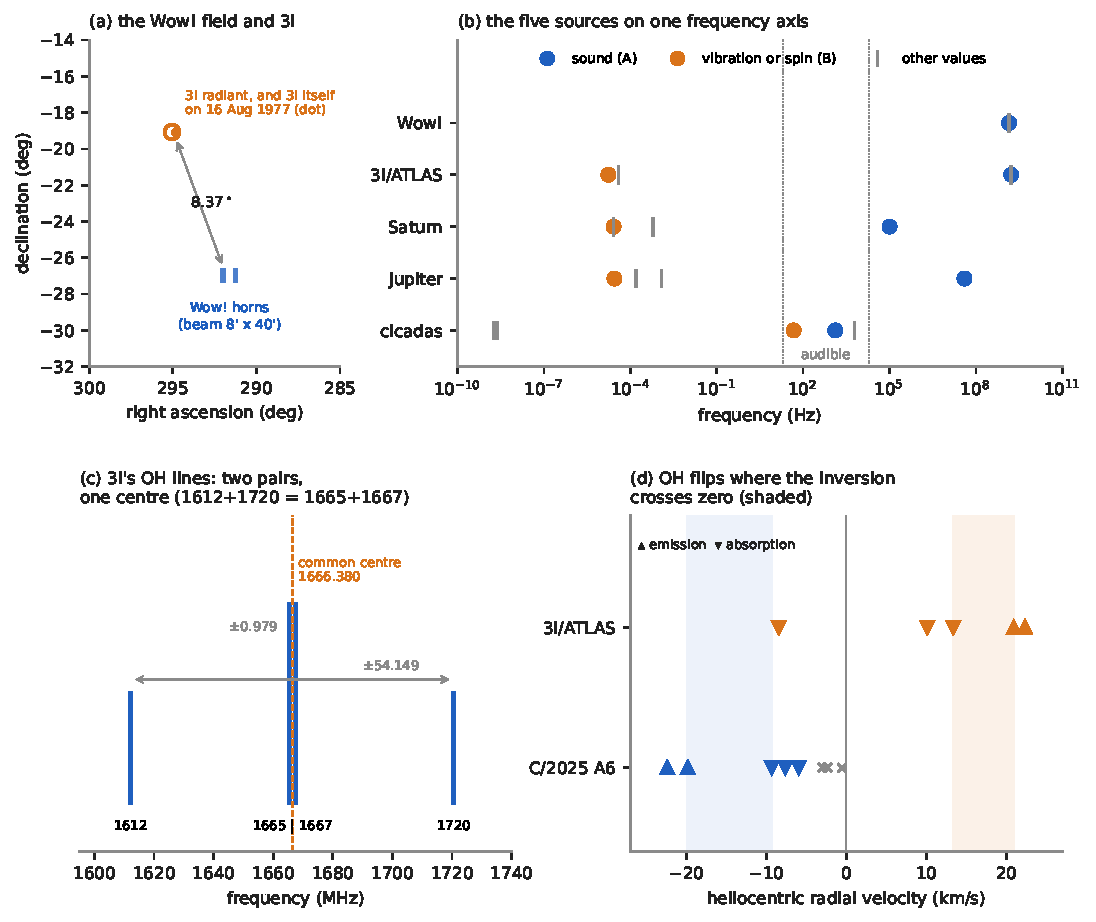
\includegraphics[width=\textwidth]{fig_sounds.pdf}
\caption{(a) The two Wow!\ horn positions with the beam footprint, and 3I's incoming direction with its 1977 position. (b) The five sources on one frequency axis: sounds (A), vibrations or spins (B) and further characteristic frequencies (grey). (c) The OH quartet: two pairs about one centre. (d) OH emission and absorption against heliocentric radial velocity for 3I/ATLAS (MeerKAT reports) and C/2025 A6 (FAST \cite{Jiang}); shading marks where each flip lies.}
\label{fig:sounds}
\end{figure}

\section{A compact centre: the planets of PSR~B1257+12}\label{sec:pulsar}
The first planets found beyond the Sun were found by arithmetic on pulse arrival times \cite{WF92}. In the timing solution of Konacki and Wolszczan \cite{KW03}, with an assumed $1.4\,M_\odot$ pulsar spinning every $6.21853$ ms, planet A has $0.020\,M_\oplus$ and a $25.262$-day period; B has $4.3\,M_\oplus$, $66.5419$ days, $e=0.0186$ and $i=53^\circ$ or $127^\circ$; C has $3.9\,M_\oplus$, $98.2114$ days, $e=0.0252$ and $i=47^\circ$ or $133^\circ$. Kepler's law puts them at $0.18849$, $0.35951$ and $0.46604$ au. The pulsar's reflex orbits, $a_\mathrm{psr}=a\,m/(M+m)=496.13$ and $583.32$ km for B and C, set against the projected semimajor axes $x=a_\mathrm{psr}\sin i/c$ of the timing solution ($1.3106$ and $1.4134$ light-ms), return $\sin i$ and $i=52.4^\circ$ and $46.6^\circ$.

\paragraph{The pair.} B and C lie near the $3{:}2$ resonance: $P_C/P_B=1.475933$, $1.60\%$ inside it, so the frequency ratio is $0.6775$ against $\frac23$. The near-resonance repeats its geometry every $1/|3/P_C-2/P_B|=5.5863$ years, and it is the planets' mutual pull in this near-resonance, seen in the timing, that fixed their true masses and inclinations \cite{KW03}. Timing cannot decide the mirror, $i$ or $180^\circ-i$: the two solutions are reflections through the plane of the sky, the observer's horizon. B and C carry $0.4912$ and $0.5072$ of the system's orbital angular momentum, and A carries $0.0017$. The ratio $L_C/L_B=(m_C/m_B)(P_C/P_B)^{1/3}=1.0325\pm0.0715$ lies within $0.45\sigma$ of $1$, treating the $\pm0.2\,M_\oplus$ mass errors as independent although they were fitted jointly. The pair is $14.31$ mutual Hill radii apart, beyond the $2\sqrt3=3.464$ that two planets on circular orbits need to avoid close encounters \cite{Gladman}; each carries the giants' two throats (\cref{tab:throats}), unequal by $h/3$ to $10^{-5}$, and its Trojans would librate in $23.09$ and $35.78$ years.

\paragraph{The centre.} A neutron star has no horizon, but its mass sets the same radii. For a non-rotating mass $M$ in Schwarzschild coordinates ($G=c=1$), light moves in the effective potential $V_\gamma=(1-2M/r)/r^2$, whose maximum $\dd V_\gamma/\dd r=-2/r^3+6M/r^4=0$ is the photon sphere $r=3M$; massive bodies move in $V=(1-2M/r)(1+L^2/r^2)$, whose circular orbits have $L^2=Mr^2/(r-3M)$ and are stable exactly for $r\ge6M$, the innermost stable circular orbit \cite{MTW}. The horizon lies at $2M$. Hence the horizon is exactly $\frac13$ of the innermost stable orbit and $\frac23$ of the photon sphere. A static observer sees circular orbits move at $v=[M/(r-2M)]^{1/2}$, exactly $c/2$ at the innermost stable orbit and $c$ at the photon sphere. For $1.4\,M_\odot$ the three radii are $4.1346$, $6.2018$ and $12.4037$ km, and the orbital frequency at the innermost stable orbit, seen from far away, is $1570.4$ Hz. A neutron-star surface at $10$--$12$ km lies between the photon sphere and the innermost stable orbit, with compactness $2GM/Rc^2$ of $0.41$--$0.34$ (\cref{fig:throats}d); the pulsar's light cylinder is at $cP/2\pi=296.708$ km.

\paragraph{The observer inside the observation.} Planet A's $25.3$-day period is close to the Sun's rotation, and Scherer and co-workers proposed that solar rotation mimicked it \cite{Scherer}; Wolszczan and co-workers weighed a planet against a heliospheric propagation effect \cite{W2000}, and the 2003 solution keeps A as a planet \cite{KW03}. A proposed fourth body was withdrawn when its signal was traced to slow changes in the dispersion measure \cite{W12}. What separates the cases is an equivalence: a companion's pull delays the pulses equally at every radio frequency, while plasma, including the observer's own solar wind, delays them as $f^{-2}$. One proposed origin of the system is a disk from the merger of two white dwarfs \cite{Podsi}: a pair merged into a centre, with planets forming around it.

\section{Discussion: the four giants as balanced pairs}\label{sec:discussion}
\Cref{tab:levels} collects the structure level by level. At every level a pair sits about a centre and balances at a zero that is either computed exactly or measured; at every level a third element or a fourth body enters in a stated way.

\begin{table}[!htb]\centering\footnotesize
\begin{tabular}{@{}>{\raggedright\arraybackslash}p{2.3cm}>{\raggedright\arraybackslash}p{3.4cm}>{\raggedright\arraybackslash}p{4.3cm}>{\raggedright\arraybackslash}p{4.4cm}@{}}\toprule
level & pair & balance (zero) & triad or fourth element\\\midrule
throats & $L_1$, $L_2$ about the planet & Hill radius; $\mathcal A=\frac h3(1-\frac{h^2}{27}+\dots)$; transmission $T=\frac12$ at the saddle & $\lambda^2-\omega^2=2$, $\lambda^2\omega^2=3^3$; 3I crossed the sphere at $1.0011\,r_H$\\
hearts & the two hemispheres; Jupiter and Saturn & winds end at $10^5$ bar in both & ring of $N$ with a centre; $3+1$ exactly on the edge\\
gas ladder & NH$_3$ and H$_2$S & $\mathrm N=\mathrm S$: neither survives & rungs $3,3,4,4$: the triad of decks, and CH$_4$ as a fourth\\
the set & Jupiter and Saturn & conjunctions at $\frac23$ of a turn & the trigon; Io, Europa, Ganymede and Callisto; three live modes and one zero mode\\
triangle & two pairs of opposite Krein sign & collision at $\mu_G$, $\omega=1/\sqrt2$ & a triad stands only around a dominant centre\\
radio & OH main and satellite pairs & common centre $1666.38040$ MHz & hydrogen: the triplet and the singlet\\
visitors & 1I, 2I, 3I & no common direction or origin & the Sun as common focus, placed by the observer\\
PSR B1257+12 & planets B and C & $L_C/L_B=1.03\pm0.07$ & horizon $\frac13$ of the ISCO; planet A as the small third\\\bottomrule
\end{tabular}
\caption{The four giants and their visitors, level by level.}\label{tab:levels}
\end{table}

\paragraph{Outlook.} We predict undiscovered retrograde irregular moons of Uranus with apocentres of $0.60$--$0.73$ of its Hill radius, $42$--$51$ million km from the planet (\cref{sec:reach}), which a deep survey of that annulus will find, and an acoustic spacing of Saturn of $112$--$117\muH$ (\cref{sec:links}), which a long continuous record of Saturn's disk or gravity will measure. A deep N/S for Neptune, from an entry probe or microwave sounding, will test \cref{thm:titration} at the second ice giant, and a measurement of the ortho/para state of hydrogen will remove the largest model uncertainty of the ice-giant ladder (up to $78\%$ in the water base) and, with O/H, place its water rung.

\section{Data and sources}\label{sec:data}
\begin{itemize}
\item \emph{Planetary constants}: NASA NSSDC planetary fact sheets for Jupiter, Saturn, Uranus and Neptune (D.~R.~Williams; updated 2 October 2024, 18 March 2025, 2 October 2024 and 3 October 2024) \cite{NSSDCJ,NSSDCS,NSSDCU,NSSDCN}: $GM$ ($126.687$, $37.931$, $5.7940$, $6.8351\times10^{6}$ km$^3$s$^{-2}$), semimajor axes ($778.479$, $1432.041$, $2867.043$, $4514.953\times10^6$ km), sidereal periods ($4332.589$ and $10759.22$ days for Jupiter and Saturn), rotation (Jupiter $9.9250$ h, Neptune $16.11$ h), equatorial radii of Uranus and Neptune ($25559$, $24764$ km), $J_2$ of Uranus and Neptune ($3343.43$, $3411\times10^{-6}$), obliquities, dipole tilts and offsets, $1$-bar and $0.1$-bar temperatures, $1$-bar gravities and bulk compositions (\cref{tab:giants,tab:ladderinputs}); Jovian and Saturnian satellite fact sheets for the moon periods \cite{NSSDCJsat,NSSDCSsat}. $GM_\odot=1.32712440018\times10^{20}$ m$^3$s$^{-2}$, within $2\times10^{-10}$ of the IAU 2009 value, and $1$ au $=149597870.7$ km \cite{IAU2009}; the planetary mass ratios $M_\odot/m$ ($1047.348644$ Jupiter, $3497.9018$ Saturn, $3098703.59$ Mars, $332946.0487$ Earth) and the Gaussian constant $0.01720209895$ used for the encounters \cite{IAU2009}.
\item \emph{Gravity fields and interiors}: Jupiter's $J_2,J_4,J_6$ \cite{Durante2020}; Saturn's $J_2,J_4,J_6$ and the Grand Finale residuals \cite{Iess}; interior models and heavy-element masses \cite{Wahl,Militzer2024,MankovichFuller}; wind depths \cite{Kaspi2018,Kaspi2020,Galanti}; p-mode signals \cite{Durante2022,Markham,Gaulme}; Uranus's rotation $17.247864$ h \cite{Lamy}.
\item \emph{Ring seismology}: Saturn's seismic rotation period, $10^\mathrm{h}33^\mathrm{m}38^\mathrm{s}$ with its $5\%$ and $95\%$ quantiles, and the counts of density and bending waves \cite{Mankovich2019}; the stably stratified core \cite{MankovichFuller}.
\item \emph{Poles}: Jupiter's cyclones \cite{Adriani,PIA,Mura,Li,Chen}; Saturn's hexagon, decagon, equinox, radio periods and dipole tilt \cite{SLHex,SLDec,SSL,AAQ,Fischer,Cao}; Jupiter's X-ray aurorae \cite{Gladstone,Dunn}.
\item \emph{Gas ladder}: all inputs of \cref{tab:ladderinputs}, with the compilations \cite{Atreya2020,AtreyaWong} and the observations \cite{Wong2004,Li2017,Li2020,Guillot2020a,Guillot2020b,Fletcher2009,Sromovsky2013,Molter2021,Irwin2018,Irwin2019a,Irwin2019b,dePater1991}; the published cloud bases of \cref{tab:validation}; secondary values quoted through these papers: the Galileo temperature profile (Seiff et al.\ 1998), the Galileo cloud base (Banfield et al.\ 1998) and the NH$_3$-ice coverage (Baines et al.\ 2002), all as quoted in \cite{AtreyaWong,Guillot2020b}, and the ice-giant CH$_4$ of Karkoschka and Tomasko, as stated in \cite{Irwin2019b}. Thermodynamic data: IAPWS equations for water \cite{WagnerPruss,Wagner2011}; the NIST Chemistry WebBook \cite{NISTWebBook} for the NH$_3$, H$_2$S and CH$_4$ triple points, sublimation enthalpies and Antoine equations, compiled there from Timmermans (1921), Fonseca and Lobo (1989), Overstreet and Giauque (1937), Stull (1947), Goodwin (1983), Clark et al.\ (1951), Giauque and Blue (1936), Stephenson and Malanowski (1987) and Prydz and Goodwin (1972); H$_2$ spectroscopic constants \cite{HuberHerzberg} and heat capacities \cite{Leachman} via the WebBook; the NH$_4$SH constant \cite{AtreyaWong}; physical constants CODATA 2018 \cite{CODATA}.
\item \emph{Sensor ladder}: the UCI Air Quality data set (hourly responses of five metal-oxide sensors with reference analysers, 10 March 2004 to 4 April 2005, $9357$ rows) \cite{UCI,DeVito}, as analysed in the chemistry companion \cite{SChem}; used here only in \cref{fig:ladder}d and \cref{sec:pairlaw}.
\item \emph{Interstellar objects}: orbital elements of 1I (JPL Small-Body Database, solution 16: $e=1.201133796$, $q_\mathrm{p}=0.2559115813$ au, $i=122.7417^\circ$, $\Omega=24.5969^\circ$, $\omega=241.8105^\circ$) \cite{JPL1I}, 2I ($e=3.3565$, $q_\mathrm{p}=2.00652$ au, $i=44.053^\circ$, $\Omega=308.15^\circ$, $\omega=209.12^\circ$, epoch JD 2458853.5) \cite{W2I} and 3I ($e=6.14135$, $q_\mathrm{p}=1.35645$ au, $i=175.12^\circ$, $\Omega=322.17^\circ$, $\omega=128.02^\circ$, epoch JD 2461090.5) \cite{W3I}; heliocentric velocities \cite{Mamajek17,TS25,dlFM25}; solar motion \cite{SBD10}; all other published properties with their sources in \cref{tab:isodir,tab:isokin,tab:isotime,tab:isophot,tab:isocomp}; JPL's 3I--Jupiter approach, $0.358330$ au at 12:22 UT on 16 March 2026 \cite{W3I}; X-ray observations of 3I \cite{ESAXRISM}; PSO~J318.5$-$22 \cite{Biller18}.
\item \emph{Radio}: the Wow!\ parameters and horn positions (Table~4 of \cite{Mendez25}); the printout code \cite{Ehman}; the hydrogen hyperfine frequency $1420405751.768\pm0.002$ Hz \cite{Hellwig}; the OH ground-state frequencies (Table~1 of \cite{Jiang}); the C/2025 A6 radial velocities and heliocentric distances (Tables~2--3 of \cite{Jiang}); MeerKAT dates and results \cite{UCT,AstroBio,ATel}; technosignature limits \cite{UCT,Sheikh,BL}; the Big Ear site, latitude $40.25^\circ$\,N, longitude $83.05^\circ$\,W (Earth-rotation velocity only, at most $0.36$ km/s).
\item \emph{Sources of sound}: Jupiter's and Saturn's radio \cite{Louis,SKAWB}; 3I's rotation \cite{SantanaRos25,ScarmatoLoeb}; cicada songs, wingbeat and broods \cite{YoungJosephson,Wan,BroodXIX}.
\item \emph{Dynamics}: Ohtsuka's captures \cite{Ohtsuka}; Trojan populations \cite{WikiMoons,dlFM,HuiTrojan,NesvornyDones}; moon lists of Jupiter (Wikipedia group tables: $13$ outer moons with eccentricities, $21$ with semimajor axes only), Saturn ($210$ Norse-group moons with eccentricities, $35$ Gallic and Inuit moons with semimajor axes only), Uranus ($29$) and Neptune ($16$), read 24 September 2026 \cite{WikiMoons}; irregular-satellite stability limits \cite{Nesvorny03}.
\item \emph{PSR~B1257+12}: the timing solution of Konacki and Wolszczan \cite{KW03}: pulse period $6.21853194840048$ ms; A: $x=0.0030$ ms, $P=25.262$ d, $0.020\,M_\oplus$; B: $x=1.3106$ ms, $e=0.0186$, $P=66.5419$ d, $\omega=250.4^\circ$, $4.3\pm0.2\,M_\oplus$, $i=53^\circ$ or $127^\circ$; C: $x=1.4134$ ms, $e=0.0252$, $P=98.2114$ d, $\omega=108.3^\circ$, $3.9\pm0.2\,M_\oplus$, $i=47^\circ$ or $133^\circ$; pulsar mass $1.4\,M_\odot$ assumed; $GM_\odot/c^2=1476.625$ m.
\item \emph{Ephemeris}: planetary positions from Schlyter's method \cite{Schlyter}, rotated to the J2000 ecliptic, validated against JPL's 3I--Jupiter, 3I--Mars and 3I--Earth approaches (\cref{sec:contact}).
\item \emph{Formulas}: Hill's problem and the restricted problem \cite{MD}; the neck topology \cite{Conley,McGehee,KLMR,Gomez}; the flux theorem \cite{MacKay}; the parabolic barrier \cite{LL}; the Gascheau--Routh criterion and Krein's theorem \cite{Gascheau,Routh,MHO}; the Laplace--Lagrange secular theory \cite{MD}; the Radau--Darwin relation \cite{MilitzerHubbard2023}; the $N+1$ vortex problem \cite{Cabral,BHW}; the Schwarzschild radii \cite{MTW}; the two-planet stability limit \cite{Gladman}.
\end{itemize}
All other numbers are computed from these inputs by the formulas and methods stated where they appear.


\begin{thebibliography}{999}\small\setlength{\itemsep}{0pt}\setlength{\parskip}{0pt}
\bibitem{Adriani} A.~Adriani et al., Clusters of cyclones encircling Jupiter's poles, \emph{Nature} 555 (2018) 216.
\bibitem{Asplund2009} M.~Asplund, N.~Grevesse, A.~J.~Sauval, P.~Scott, The chemical composition of the Sun, \emph{Annu. Rev. Astron. Astrophys.} 47 (2009) 481--522.
\bibitem{AstroBio} Astrobiology.com, South African telescope detects natural radio emission, and no signal of technological origin, from interstellar visitor 3I/ATLAS, 21 December 2025, \url{https://astrobiology.com/2025/12/21/south-african-telescope-detects-natural-radio-emission-and-no-signal-of-technological-origin-from-interstellar-visitor-3i-atlas/} (accessed 24 September 2026).
\bibitem{AAQ} Astronomical Association of Queensland, Saturn in 2024/2025 and the next edge-on appearance of its rings, \url{https://www.aaq.org.au/saturn-in-2024-2025-and-the-next-edge-on-appearance-of-its-rings/} (accessed 24 September 2026).
\bibitem{Atreya2020} S.~K.~Atreya, M.~H.~Hofstadter, J.~H.~In, O.~Mousis, K.~Reh, M.~H.~Wong, Deep atmosphere composition, structure, origin, and exploration, with particular focus on critical in situ science at the icy giants, \emph{Space Sci. Rev.} 216 (2020) 18.
\bibitem{AtreyaWong} S.~K.~Atreya, A.-S.~Wong, Coupled clouds and chemistry of the giant planets---a case for multiprobes, \emph{Space Sci. Rev.} 116 (2005) 121--136.
\bibitem{Bagnulo21} S.~Bagnulo et al., Unusually high polarization of 2I/Borisov, \emph{Nat. Commun.} 12 (2021) 1797.
\bibitem{BJ20} C.~A.~L.~Bailer-Jones et al., A search for the origin of the interstellar comet 2I/Borisov, \emph{Astron. Astrophys.} 634 (2020) A14.
\bibitem{BHW} A.~M.~Barry, G.~R.~Hall, C.~E.~Wayne, Relative equilibria of the $(1+N)$-vortex problem, \emph{J. Nonlinear Sci.} 22 (2012) 63--83.
\bibitem{BS23} J.~B.~Bergner, D.~Z.~Seligman, Acceleration of 1I/\textquoteleft Oumuamua from radiolytically produced H$_2$ in H$_2$O ice, \emph{Nature} 615 (2023) 610--613.
\bibitem{Biller18} B.~A.~Biller et al., Simultaneous multiwavelength variability characterization of the free-floating planetary-mass object PSO J318.5$-$22, \emph{Astron. J.} 155 (2018) 95.
\bibitem{Bodewits20} D.~Bodewits et al., The carbon monoxide-rich interstellar comet 2I/Borisov, \emph{Nat. Astron.} 4 (2020) 867--871.
\bibitem{Bolin18} B.~T.~Bolin et al., APO time-resolved color photometry of highly elongated interstellar object 1I/\textquoteleft Oumuamua, \emph{Astrophys. J. Lett.} 852 (2018) L2.
\bibitem{BL} Breakthrough Listen, Observations of interstellar object 3I/ATLAS, \url{https://seti.berkeley.edu/atlas} (accessed 24 September 2026).
\bibitem{Cabral} H.~E.~Cabral, D.~S.~Schmidt, Stability of relative equilibria in the problem of $N+1$ vortices, \emph{SIAM J. Math. Anal.} 31 (1999) 231--250.
\bibitem{Cao} H.~Cao et al., The landscape of Saturn's internal magnetic field from the Cassini Grand Finale, \emph{Icarus} 344 (2020) 113541.
\bibitem{Dio} Cassius Dio, \emph{Roman History}, Book XXXVII, chapters 18--19, translated by E.~Cary, Loeb Classical Library, Vol.~III, Harvard University Press, Cambridge MA, 1914.
\bibitem{Chen} S.~Chen, A.~P.~Ingersoll, C.~Li, Jupiter's polar vortex crystals explored using the shallow water equations, arXiv:2403.00870 (2024).
\bibitem{CODATA} E.~Tiesinga, P.~J.~Mohr, D.~B.~Newell, B.~N.~Taylor, CODATA recommended values of the fundamental physical constants: 2018, \emph{Rev. Mod. Phys.} 93 (2021) 025010.
\bibitem{Conley} C.~Conley, Low energy transit orbits in the restricted three-body problem, \emph{SIAM J. Appl. Math.} 16 (1968) 732--746.
\bibitem{Cordiner20} M.~A.~Cordiner et al., Unusually high CO abundance of the first active interstellar comet, \emph{Nat. Astron.} 4 (2020) 861--866.
\bibitem{Cordiner25} M.~A.~Cordiner et al., JWST detection of a carbon dioxide dominated gas coma surrounding interstellar object 3I/ATLAS, \emph{Astrophys. J. Lett.} (2025), arXiv:2508.18209.
\bibitem{dlFM} C.~de la Fuente Marcos, R.~de la Fuente Marcos, Asteroid 2014 YX$_{49}$: a large transient Trojan of Uranus, \emph{Mon. Not. R. Astron. Soc.} 467 (2017) 1561--1568.
\bibitem{dlFM25} C.~de la Fuente Marcos et al., Assessing interstellar comet 3I/ATLAS with the 10.4 m Gran Telescopio Canarias and the Two-meter Twin Telescope, \emph{Astron. Astrophys.} 700 (2025) L9.
\bibitem{dePater1991} I.~de Pater, P.~N.~Romani, S.~K.~Atreya, Possible microwave absorption by H$_2$S gas in Uranus' and Neptune's atmospheres, \emph{Icarus} 91 (1991) 220--233.
\bibitem{DeVito} S.~De Vito, E.~Massera, M.~Piga, L.~Martinotto, G.~Di Francia, On field calibration of an electronic nose for benzene estimation in an urban pollution monitoring scenario, \emph{Sens. Actuators B} 129 (2008) 750--757.
\bibitem{UCI} S.~De Vito, Air Quality [data set], UCI Machine Learning Repository, 2008, doi:10.24432/C59K5F, \url{https://archive.ics.uci.edu/dataset/360/air+quality} (accessed 24 September 2026).
\bibitem{Deam26} S.~E.~Deam, M.~T.~Bannister, C.~Opitom et al., A portrait throughout perihelion of the NH$_2$-rich interstellar comet 2I/Borisov, \emph{Planet. Sci. J.} 7 (2026) 88.
\bibitem{Despois} D.~Despois, E.~Gerard, J.~Crovisier, I.~Kazes, \emph{Astron. Astrophys.} 99 (1981) 320.
\bibitem{Dunn} W.~R.~Dunn et al., The independent pulsations of Jupiter's northern and southern X-ray auroras, \emph{Nat. Astron.} 1 (2017) 758--764.
\bibitem{Durante2020} D.~Durante et al., Jupiter's gravity field halfway through the Juno mission, \emph{Geophys. Res. Lett.} 47 (2020) e2019GL086572.
\bibitem{Durante2022} D.~Durante et al., Juno spacecraft gravity measurements provide evidence for normal modes of Jupiter, \emph{Nat. Commun.} 13 (2022) 4632.
\bibitem{Ehman} J.~R.~Ehman, The Big Ear Wow! signal: what we know and don't know about it after 30 years, \url{http://www.bigear.org/Wow30th/wow30th.htm} (accessed 24 September 2026).
\bibitem{ER} A.~Einstein, N.~Rosen, The particle problem in the general theory of relativity, \emph{Phys. Rev.} 48 (1935) 73--77.
\bibitem{ESAXRISM} ESA, XRISM sees Comet 3I/ATLAS in X-ray light, December 2025, \url{https://www.esa.int/ESA_Multimedia/Images/2025/12/XRISM_sees_Comet_3I_ATLAS_in_X-ray_light} (accessed 24 September 2026).
\bibitem{Feinstein25} A.~D.~Feinstein, J.~W.~Noonan, D.~Z.~Seligman, Precovery observations of 3I/ATLAS from TESS suggest possible distant activity, \emph{Astrophys. J. Lett.} 991 (2025) L2.
\bibitem{SKAWB} C.~Ferrari et al. (eds), French SKA White Book: the French community towards the Square Kilometre Array, arXiv:1712.06950 (2017), Sect.~2.4 (P.~Zarka et al.).
\bibitem{Fienga} A.~Fienga, J.~Laskar, H.~Manche, M.~Gastineau, Constraints on the location of a possible 9th planet derived from the Cassini data, \emph{Astron. Astrophys.} 587 (2016) L8.
\bibitem{Fischer} G.~Fischer, D.~A.~Gurnett, W.~S.~Kurth, S.-Y.~Ye, J.~B.~Groene, Saturn kilometric radiation periodicity after equinox, \emph{Icarus} 254 (2015) 72--91.
\bibitem{Fletcher2009} L.~N.~Fletcher, G.~S.~Orton, N.~A.~Teanby, P.~G.~J.~Irwin, G.~L.~Bjoraker, Methane and its isotopologues on Saturn from Cassini/CIRS observations, \emph{Icarus} 199 (2009) 351--367.
\bibitem{Galanti} E.~Galanti et al., Saturn's deep atmospheric flows revealed by the Cassini Grand Finale gravity measurements, \emph{Geophys. Res. Lett.} 46 (2019) 616--624.
\bibitem{Gascheau} G.~Gascheau, Examen d'une classe d'\'equations diff\'erentielles et applications \`a un cas particulier du probl\`eme des trois corps, \emph{C. R. Acad. Sci. Paris} 16 (1843) 393.
\bibitem{Gaulme} P.~Gaulme et al., Detection of Jovian seismic waves: a new probe of its interior structure, \emph{Astron. Astrophys.} 531 (2011) A104.
\bibitem{Gladman} B.~Gladman, Dynamics of systems of two close planets, \emph{Icarus} 106 (1993) 247.
\bibitem{Gladstone} G.~R.~Gladstone et al., A pulsating auroral X-ray hot spot on Jupiter, \emph{Nature} 415 (2002) 1000--1003.
\bibitem{Gomez} G.~G\'omez, W.~S.~Koon, M.~W.~Lo, J.~E.~Marsden, J.~Masdemont, S.~D.~Ross, Invariant manifolds, the spatial three-body problem and space mission design, AAS/AIAA Astrodynamics Specialist Conference, paper AAS 01-301 (2001).
\bibitem{Gray25} Z.~Gray et al., Extreme negative polarization of new interstellar comet 3I/ATLAS, \emph{Astrophys. J. Lett.} 992 (2025) L29.
\bibitem{Guido} A.~F.~Guido, C.~Efthymiopoulos, Arches of chaos, heteroclinic connections of first-order MMRs, and the chaotic transport of small bodies in the Sun--Jupiter system, \emph{Celest. Mech. Dyn. Astron.} 138 (2026) 32.
\bibitem{Guillot2020a} T.~Guillot, D.~J.~Stevenson, S.~K.~Atreya, S.~J.~Bolton, H.~N.~Becker, Storms and the depletion of ammonia in Jupiter: I. Microphysics of ``mushballs'', \emph{J. Geophys. Res. Planets} 125 (2020) e2020JE006403.
\bibitem{Guillot2020b} T.~Guillot, C.~Li, S.~J.~Bolton, S.~T.~Brown, A.~P.~Ingersoll, M.~A.~Janssen, S.~M.~Levin, J.~I.~Lunine, G.~S.~Orton, P.~G.~Steffes, D.~J.~Stevenson, Storms and the depletion of ammonia in Jupiter: II. Explaining the Juno observations, \emph{J. Geophys. Res. Planets} 125 (2020) e2020JE006404.
\bibitem{GD21} P.~Guzik, M.~Drahus, Gaseous atomic nickel in the coma of interstellar comet 2I/Borisov, \emph{Nature} 593 (2021) 375--378.
\bibitem{HP22} O.~Harrington Pinto et al., A survey of CO, CO$_2$, and H$_2$O in comets and Centaurs, \emph{Planet. Sci. J.} 3 (2022) 247.
\bibitem{Hellwig} H.~Hellwig, R.~F.~C.~Vessot, M.~W.~Levine, P.~W.~Zitzewitz, D.~W.~Allan, D.~J.~Glaze, Measurement of the unperturbed hydrogen hyperfine transition frequency, \emph{IEEE Trans. Instrum. Meas.} IM-19 (1970) 200.
\bibitem{Hopkins25} M.~J.~Hopkins et al., From a different star: 3I/ATLAS in the context of the \=Otautahi--Oxford interstellar object population model, \emph{Astrophys. J. Lett.} 990 (2025) L30.
\bibitem{HuberHerzberg} K.~P.~Huber, G.~Herzberg, \emph{Molecular Spectra and Molecular Structure IV. Constants of Diatomic Molecules}, Van Nostrand Reinhold, New York, 1979.
\bibitem{Hui20} M.-T.~Hui et al., Physical characterization of interstellar comet 2I/2019 Q4 (Borisov), \emph{Astron. J.} 160 (2020) 92.
\bibitem{HuiTrojan} M.-T.~Hui, P.~A.~Wiegert et al., 2019 UO$_{14}$: a transient Trojan of Saturn, \emph{Astrophys. J. Lett.} 975 (2024) L3.
\bibitem{Hui26} M.-T.~Hui, D.~Jewitt, M.~J.~Mutchler, J.~Agarwal, Y.~Kim, Nucleus and postperihelion activity of interstellar object 3I/ATLAS observed by the Hubble Space Telescope, \emph{Astrophys. J. Lett.} 999 (2026) L37.
\bibitem{Hutsemekers26} D.~Hutsem\'ekers et al., Pre-perihelion evolution of the Ni\,\textsc{i}/Fe\,\textsc{i} abundance ratio in the coma of the interstellar comet 3I/ATLAS: from extreme to normal, \emph{Astron. Astrophys.} 706 (2026) A43.
\bibitem{Iess} L.~Iess et al., Measurement and implications of Saturn's gravity field and ring mass, \emph{Science} 364 (2019) eaat2965.
\bibitem{Irwin2018} P.~G.~J.~Irwin, D.~Toledo, R.~Garland, N.~A.~Teanby, L.~N.~Fletcher, G.~A.~Orton, B.~B\'ezard, Detection of hydrogen sulfide above the clouds in Uranus's atmosphere, \emph{Nat. Astron.} 2 (2018) 420--427.
\bibitem{Irwin2019a} P.~G.~J.~Irwin, D.~Toledo, R.~Garland, N.~A.~Teanby, L.~N.~Fletcher, G.~S.~Orton, B.~B\'ezard, Probable detection of hydrogen sulphide (H$_2$S) in Neptune's atmosphere, \emph{Icarus} 321 (2019) 550--563.
\bibitem{Irwin2019b} P.~G.~J.~Irwin, D.~Toledo, A.~S.~Braude, R.~Bacon, P.~M.~Weilbacher, N.~A.~Teanby, L.~N.~Fletcher, G.~S.~Orton, Latitudinal variation in the abundance of methane (CH$_4$) above the clouds in Neptune's atmosphere from VLT/MUSE Narrow Field Mode observations, \emph{Icarus} 331 (2019) 69--82.
\bibitem{ISSI19} The \textquoteleft Oumuamua ISSI Team, The natural history of \textquoteleft Oumuamua, \emph{Nat. Astron.} 3 (2019) 594--602.
\bibitem{JD21} A.~P.~Jackson, S.~J.~Desch, 1I/\textquoteleft Oumuamua as an N$_2$ ice fragment of an exo-Pluto surface: I. Size and compositional constraints, \emph{J. Geophys. Res. Planets} 126 (2021) e2020JE006706.
\bibitem{Jaffe} C.~Jaff\'e, S.~D.~Ross, M.~W.~Lo, J.~Marsden, D.~Farrelly, T.~Uzer, Statistical theory of asteroid escape rates, \emph{Phys. Rev. Lett.} 89 (2002) 011101.
\bibitem{JamesWormhole} O.~James, E.~von Tunzelmann, P.~Franklin, K.~S.~Thorne, Visualizing Interstellar's wormhole, \emph{Am. J. Phys.} 83 (2015) 486.
\bibitem{JPL1I} NASA Jet Propulsion Laboratory, Small-Body Database, 1I/\textquoteleft Oumuamua (A/2017 U1), orbit solution 16, \url{https://ssd.jpl.nasa.gov/tools/sbdb_lookup.html#/?sstr=1I} (accessed 24 September 2026).
\bibitem{Jewitt20} D.~Jewitt et al., The nucleus of interstellar comet 2I/Borisov, \emph{Astrophys. J. Lett.} 888 (2020) L23.
\bibitem{Jiang} D.~Jiang et al., From emission to absorption: the FAST observation of the OH 18-cm lines from the comet C/2025 A6, arXiv:2512.21969 (2025).
\bibitem{KL26} S.~Kakharov, A.~Loeb, Galactic trajectories of interstellar objects 1I/\textquoteleft Oumuamua, 2I/Borisov, and 3I/ATLAS, \emph{Astron. Astrophys.} 709 (2026) A178, arXiv:2408.02739.
\bibitem{Kaspi2018} Y.~Kaspi et al., Jupiter's atmospheric jet streams extend thousands of kilometres deep, \emph{Nature} 555 (2018) 223--226.
\bibitem{Kaspi2020} Y.~Kaspi et al., Comparison of the deep atmospheric dynamics of Jupiter and Saturn in light of the Juno and Cassini gravity measurements, \emph{Space Sci. Rev.} 216 (2020) 84.
\bibitem{KW03} M.~Konacki, A.~Wolszczan, Masses and orbital inclinations of planets in the PSR B1257+12 system, \emph{Astrophys. J.} 591 (2003) L147.
\bibitem{KLMR} W.~S.~Koon, M.~W.~Lo, J.~E.~Marsden, S.~D.~Ross, Dynamical systems, the three-body problem and space mission design, in: \emph{Equadiff 99}, World Scientific, Singapore, 2000, 1167--1181.
\bibitem{Lamy} L.~Lamy et al., A new rotation period and longitude system for Uranus, \emph{Nat. Astron.} 9 (2025) 658--665.
\bibitem{LL} L.~D.~Landau, E.~M.~Lifshitz, \emph{Quantum Mechanics: Non-relativistic Theory}, 3rd ed., Pergamon, Oxford, 1977.
\bibitem{Leachman} J.~W.~Leachman, R.~T.~Jacobsen, S.~G.~Penoncello, E.~W.~Lemmon, Fundamental equations of state for parahydrogen, normal hydrogen, and orthohydrogen, \emph{J. Phys. Chem. Ref. Data} 38 (2009) 721--748.
\bibitem{Lewis1969} J.~S.~Lewis, The clouds of Jupiter and the NH$_3$--H$_2$O and NH$_3$--H$_2$S systems, \emph{Icarus} 10 (1969) 365--378.
\bibitem{Li2017} C.~Li et al., The distribution of ammonia on Jupiter from a preliminary inversion of Juno microwave radiometer data, \emph{Geophys. Res. Lett.} 44 (2017) 5317--5325.
\bibitem{Li2020} C.~Li et al., The water abundance in Jupiter's equatorial zone, \emph{Nat. Astron.} 4 (2020) 609--616.
\bibitem{Li} C.~Li, A.~P.~Ingersoll, A.~P.~Klipfel, H.~Brettle, Modeling the stability of polygonal patterns of vortices at the poles of Jupiter as revealed by the Juno spacecraft, \emph{Proc. Natl. Acad. Sci. USA} 117 (2020) 24082--24087.
\bibitem{NISTWebBook} P.~J.~Linstrom (ed.), \emph{NIST Chemistry WebBook}, NIST Standard Reference Database 69, National Institute of Standards and Technology, Gaithersburg MD, doi:10.18434/T4D303, \url{https://webbook.nist.gov} (accessed 24 September 2026).
\bibitem{LoebWow} A.~Loeb, Was the ``Wow! signal'' emitted from 3I/ATLAS?, \url{https://avi-loeb.medium.com} (2025, accessed 24 September 2026).
\bibitem{LoebJuno} A.~Loeb, A.~Hibberd, A.~Crowl, Intercepting 3I/ATLAS at its closest approach to Jupiter with the Juno spacecraft, \emph{Aerospace} 12 (2025) 851.
\bibitem{Louis} C.~K.~Louis, L.~Lamy, P.~Zarka, B.~Cecconi, S.~L.~G.~Hess, X.~Bonnin, Simulating Jupiter--satellite decametric emissions with ExPRES: a parametric study, arXiv:1804.10499 (2018).
\bibitem{IAU2009} B.~Luzum et al., The IAU 2009 system of astronomical constants: the report of the IAU working group on numerical standards for Fundamental Astronomy, \emph{Celest. Mech. Dyn. Astron.} 110 (2011) 293--304.
\bibitem{MacKay} R.~S.~MacKay, Flux over a saddle, \emph{Phys. Lett. A} 145 (1990) 425--427.
\bibitem{Mamajek17} E.~Mamajek, Kinematics of the interstellar vagabond 1I/\textquoteleft Oumuamua (A/2017 U1), \emph{Res. Notes AAS} 1 (2017) 21.
\bibitem{Manfroid21} J.~Manfroid et al., Iron and nickel atoms in cometary atmospheres even far from the Sun, \emph{Nature} 593 (2021) 372--374.
\bibitem{Mankovich2019} C.~Mankovich, M.~S.~Marley, J.~J.~Fortney, N.~Movshovitz, Cassini ring seismology as a probe of Saturn's interior. I. Rigid rotation, \emph{Astrophys. J.} 871 (2019) 1.
\bibitem{MankovichFuller} C.~R.~Mankovich, J.~Fuller, A diffuse core in Saturn revealed by ring seismology, \emph{Nat. Astron.} 5 (2021) 1103.
\bibitem{Markham} S.~Markham, D.~Durante, L.~Iess, D.~Stevenson, Possible evidence of p-modes in Cassini measurements of Saturn's gravity field, \emph{Planet. Sci. J.} 1 (2020) 27.
\bibitem{McGehee} R.~McGehee, Some homoclinic orbits for the restricted three-body problem, Ph.D. thesis, University of Wisconsin, Madison, 1969.
\bibitem{Meech17} K.~J.~Meech et al., A brief visit from a red and extremely elongated interstellar asteroid, \emph{Nature} 552 (2017) 378--381.
\bibitem{Mendez24} A.~M\'endez, K.~Ortiz Ceballos, J.~I.~Zuluaga, Arecibo Wow! I: an astrophysical explanation for the Wow! signal, arXiv:2408.08513 (2024).
\bibitem{Mendez25} A.~M\'endez et al., Arecibo Wow! II: revised properties of the Wow! signal from archival Ohio SETI data, arXiv:2508.10657 (2025).
\bibitem{MHO} K.~R.~Meyer, G.~R.~Hall, D.~Offin, \emph{Introduction to Hamiltonian Dynamical Systems and the N-Body Problem}, 2nd ed., Applied Mathematical Sciences 90, Springer, New York, 2009.
\bibitem{Micheli18} M.~Micheli et al., Non-gravitational acceleration in the trajectory of 1I/2017 U1 (\textquoteleft Oumuamua), \emph{Nature} 559 (2018) 223--226.
\bibitem{MilitzerHubbard2023} B.~Militzer, W.~B.~Hubbard, Relation of gravity, winds, and the moment of inertia of Jupiter and Saturn, \emph{Planet. Sci. J.} 4 (2023) 95.
\bibitem{Militzer2024} B.~Militzer, W.~B.~Hubbard, Study of Jupiter's interior: comparison of 2, 3, 4, 5, and 6 layer models, \emph{Icarus} 411 (2024) 115955.
\bibitem{MPEC19} Minor Planet Center, MPEC 2019-R106, 11 September 2019.
\bibitem{MPEC25} Minor Planet Center, MPEC 2025-N12, 2 July 2025.
\bibitem{MTW} C.~W.~Misner, K.~S.~Thorne, J.~A.~Wheeler, \emph{Gravitation}, Freeman, San Francisco, 1973.
\bibitem{Molter2021} E.~M.~Molter, I.~de Pater, S.~Luszcz-Cook, J.~Tollefson, R.~J.~Sault, B.~Butler, D.~de Boer, Tropospheric composition and circulation of Uranus with ALMA and the VLA, \emph{Planet. Sci. J.} 2 (2021) 3.
\bibitem{Mura} A.~Mura et al., Oscillations and stability of the Jupiter polar cyclones, \emph{Geophys. Res. Lett.} 48 (2021) e2021GL094235.
\bibitem{MD} C.~D.~Murray, S.~F.~Dermott, \emph{Solar System Dynamics}, Cambridge University Press, Cambridge, 1999.
\bibitem{PIA} NASA/JPL, Jupiter's pentagon turns hexagon (PIA23559), \url{https://www.jpl.nasa.gov/images/pia23559-jupiters-pentagon-turns-hexagon/} (accessed 24 September 2026).
\bibitem{NSSDCJsat} D.~R.~Williams, Jovian Satellite Fact Sheet, NASA Space Science Data Coordinated Archive, \url{https://nssdc.gsfc.nasa.gov/planetary/factsheet/joviansatfact.html} (accessed 24 September 2026).
\bibitem{NSSDCSsat} D.~R.~Williams, Saturnian Satellite Fact Sheet, NASA Space Science Data Coordinated Archive, \url{https://nssdc.gsfc.nasa.gov/planetary/factsheet/saturniansatfact.html} (accessed 24 September 2026).
\bibitem{NesvornyDones} D.~Nesvorn\'y, L.~Dones, How long-lived are the hypothetical Trojan populations of Saturn, Uranus, and Neptune?, \emph{Icarus} 160 (2002) 271--288.
\bibitem{Nesvorny03} D.~Nesvorn\'y, J.~L.~A.~Alvarellos, L.~Dones, H.~F.~Levison, Orbital and collisional evolution of the irregular satellites, \emph{Astron. J.} 126 (2003) 398--429.
\bibitem{Ohtsuka} K.~Ohtsuka, T.~Ito, M.~Yoshikawa, D.~J.~Asher, H.~Arakida, Quasi-Hilda comet 147P/Kushida--Muramatsu: another long temporary satellite capture by Jupiter, \emph{Astron. Astrophys.} 489 (2008) 1355--1362.
\bibitem{Opitom21} C.~Opitom et al., The similarity of the interstellar comet 2I/Borisov to Solar System comets from high-resolution optical spectroscopy, \emph{Astron. Astrophys.} 650 (2021) L19.
\bibitem{Opitom26} C.~Opitom et al., High nitrogen and carbon isotopic ratios in the interstellar comet 3I/ATLAS, \emph{Nat. Astron.} (2026), doi:10.1038/s41550-026-02921-7.
\bibitem{Paek26} G.~S.~H.~Paek et al., Pre-perihelion emergence of the CN gas coma in 3I/ATLAS temporally and spatially resolved by the 7-dimensional Telescope, \emph{Astrophys. J.} (2026), doi:10.3847/1538-4357/ae47f0, arXiv:2602.12930.
\bibitem{ATel} D.~J.~Pisano et al., Detection of 1665/1667 MHz OH absorption in 3I/ATLAS, \emph{Astronomer's Telegram} 17473 (2025).
\bibitem{Podsi} P.~Podsiadlowski, Planet formation scenarios, in: \emph{Planets around Pulsars}, ASP Conf. Ser. 36 (1993) 149--165.
\bibitem{PorterCv} M.~A.~Porter, P.~Cvitanovi\'c, Ground control to Niels Bohr: exploring outer space with atomic physics, \emph{Notices Amer. Math. Soc.} 52 (2005) 1020--1025.
\bibitem{Rahat25} R.~Rahatgaonkar et al., Very Large Telescope observations of interstellar comet 3I/ATLAS. II. From quiescence to glow: dramatic rise of Ni\,\textsc{i} emission and incipient CN outgassing at large heliocentric distances, \emph{Astrophys. J. Lett.} 995 (2025) L34.
\bibitem{Routh} E.~J.~Routh, On Laplace's three particles, with a supplement on the stability of steady motion, \emph{Proc. London Math. Soc.} 6 (1874) 86--97.
\bibitem{SLHex} A.~S\'anchez-Lavega et al., The long-term steady motion of Saturn's hexagon and the stability of its enclosed jet stream under seasonal changes, \emph{Geophys. Res. Lett.} 41 (2014) 1425.
\bibitem{SLDec} A.~S\'anchez-Lavega et al., A decagon wave around Saturn's south pole, \emph{Sci. Adv.} 12 (2026) eaee4251.
\bibitem{SantanaRos25} T.~Santana-Ros et al., Temporal evolution of the third interstellar comet 3I/ATLAS: spin, color, spectra, and dust activity, \emph{Astron. Astrophys.} 702 (2025) L3.
\bibitem{ScarmatoLoeb} T.~Scarmato, A.~Loeb, Rotation period of 3I/ATLAS after perihelion from jet position angle wobble and photometric variability, arXiv:2601.10860 (2026).
\bibitem{Scherer} K.~Scherer, H.~Fichtner, J.~D.~Anderson, E.~L.~Lau, A pulsar, the heliosphere, and Pioneer 10: probable mimicking of a planet of PSR B1257+12 by solar rotation, \emph{Science} 278 (1997) 1919.
\bibitem{Schleicher} D.~G.~Schleicher, M.~F.~A'Hearn, \emph{Astrophys. J.} 331 (1988) 1058.
\bibitem{Schlyter} P.~Schlyter, How to compute planetary positions, \url{https://stjarnhimlen.se/comp/ppcomp.html} (accessed 24 September 2026).
\bibitem{SBD10} R.~Sch\"onrich, J.~Binney, W.~Dehnen, Local kinematics and the local standard of rest, \emph{Mon. Not. R. Astron. Soc.} 403 (2010) 1829--1833.
\bibitem{Seligman25} D.~Z.~Seligman et al., Discovery and preliminary characterization of a third interstellar object: 3I/ATLAS, \emph{Astrophys. J. Lett.} 989 (2025) L36.
\bibitem{Sheikh} S.~Z.~Sheikh et al., A search for radio technosignatures from interstellar object 3I/ATLAS with the Allen Telescope Array, arXiv:2512.18142 (2025).
\bibitem{Shinnaka26} Y.~Shinnaka et al., A post-perihelion constraint on the CO$_2$/H$_2$O ratio of interstellar comet 3I/ATLAS from [O\,\textsc{i}] forbidden lines, arXiv:2603.25002 (2026).
\bibitem{Sicardy} B.~Sicardy, Stability of the triangular Lagrange points beyond Gascheau's value, \emph{Celest. Mech. Dyn. Astron.} 107 (2010) 145--155.
\bibitem{SMath} A.~Singh, Pair Balance and the Riemann Zeros: The Signed Current, the Mirror and the Merge, and the Prime Two, manuscript, 25 September 2026.
\bibitem{SPhys} A.~Singh, The Reversible Half and the Third Body: Pairs and Triads in Measurement Records and the Three-Body Problem, manuscript, 25 September 2026.
\bibitem{SQuant} A.~Singh, The Riemann Kernel as a Quantum State: Wigner Negativity, Decoherence at the Thirds and Lee--Yang Zeros, manuscript, 25 September 2026.
\bibitem{SChem} A.~Singh, Which Member Carries: Two-State Pairs from Atoms to Gas Sensors, and D\"obereiner's Triads as Balanced Pairs, manuscript, 25 September 2026.
\bibitem{SAlg} A.~Singh, Three Is Enough: Radix Economy, Balanced-Ternary Arithmetic and Ternary-Weight Networks, manuscript, 25 September 2026.
\bibitem{SZero} A.~Singh, What a Zero Is: One Involution across Mathematics, Physics, Chemistry, Neuroscience, Computation and the Giant Planets, manuscript, 25 September 2026.
\bibitem{Spada26} L.~Spada, M.~Kr\'olikowska, L.~Dones, Systematic and statistical uncertainties in the non-gravitational acceleration of 3I/ATLAS, arXiv:2603.00782 (2026).
\bibitem{Sromovsky2013} L.~A.~Sromovsky, K.~H.~Baines, P.~M.~Fry, Saturn's Great Storm of 2010--2011: evidence for ammonia and water ices from analysis of VIMS spectra, \emph{Icarus} 226 (2013) 402--418.
\bibitem{TS25} A.~G.~Taylor, D.~Z.~Seligman, The kinematic age of 3I/ATLAS and its implications for early planet formation, \emph{Astrophys. J. Lett.} 990 (2025) L14.
\bibitem{Thomson} J.~J.~Thomson, \emph{A Treatise on the Motion of Vortex Rings}, Macmillan, London, 1883.
\bibitem{Thoss26} V.~Thoss, A.~Loeb, A.~Burkert, Inferring the mass and size of 3I/ATLAS from its non-gravitational acceleration, arXiv:2603.15735 (2026).
\bibitem{Todorovic} N.~Todorovi\'c, D.~Wu, A.~J.~Rosengren, The arches of chaos in the Solar System, \emph{Sci. Adv.} 6 (2020) eabd1313.
\bibitem{Trilling18} D.~E.~Trilling et al., Spitzer observations of interstellar object 1I/\textquoteleft Oumuamua, \emph{Astron. J.} 156 (2018) 261.
\bibitem{SSL} UC Berkeley Space Sciences Laboratory, Decagon wave emerges near Saturn's south pole, September 2026, \url{https://www.ssl.berkeley.edu/decagon-wave-emerges-near-saturns-south-pole/} (accessed 24 September 2026).
\bibitem{UCT} University of Cape Town, UCT collaborates with SARAO as MeerKAT decodes interstellar visitor 3I/ATLAS, UCT News, 20 November 2025, \url{https://www.news.uct.ac.za} (accessed 24 September 2026).
\bibitem{Wagner2011} W.~Wagner, T.~Riethmann, R.~Feistel, A.~H.~Harvey, New equations for the sublimation pressure and melting pressure of H$_2$O ice Ih, \emph{J. Phys. Chem. Ref. Data} 40 (2011) 043103.
\bibitem{WagnerPruss} W.~Wagner, A.~Pruss, International equations for the saturation properties of ordinary water substance. Revised according to the International Temperature Scale of 1990, \emph{J. Phys. Chem. Ref. Data} 22 (1993) 783--787.
\bibitem{Wahl} S.~M.~Wahl et al., Comparing Jupiter interior structure models to Juno gravity measurements and the role of a dilute core, \emph{Geophys. Res. Lett.} 44 (2017) 4649--4659.
\bibitem{Wan} H.~Wan, H.~Dong, K.~Gai, Computational investigation of cicada aerodynamics in forward flight, \emph{J. R. Soc. Interface} 12 (2015) 20141116.
\bibitem{WL73} S.~J.~Weidenschilling, J.~S.~Lewis, Atmospheric and cloud structures of the Jovian planets, \emph{Icarus} 20 (1973) 465--476.
\bibitem{BroodXIX} Wikipedia, Brood XIX, \url{https://en.wikipedia.org/wiki/Brood_XIX} (accessed 24 September 2026).
\bibitem{WikiMoons} Wikipedia, Moons of Jupiter; Moons of Saturn; Moons of Uranus; Moons of Neptune; Norse group; Neptune trojan, \url{https://en.wikipedia.org/wiki/Moons_of_Jupiter} and the linked pages (accessed 24 September 2026).
\bibitem{W2I} JPL orbit of 2I/Borisov (epoch JD 2458853.5), as quoted at \url{https://en.wikipedia.org/wiki/2I/Borisov} (accessed 24 September 2026).
\bibitem{W3I} JPL orbit and close-approach data of 3I/ATLAS (epoch JD 2461090.5), as quoted at \url{https://en.wikipedia.org/wiki/3I/ATLAS} (accessed 24 September 2026).
\bibitem{WaterHole} Wikipedia, Water hole (radio), \url{https://en.wikipedia.org/wiki/Water_hole_(radio)} (accessed 24 September 2026).
\bibitem{NSSDCJ} D.~R.~Williams, Jupiter Fact Sheet, NASA Space Science Data Coordinated Archive, updated 2 October 2024, \url{https://nssdc.gsfc.nasa.gov/planetary/factsheet/jupiterfact.html} (accessed 24 September 2026).
\bibitem{NSSDCN} D.~R.~Williams, Neptune Fact Sheet, NASA Space Science Data Coordinated Archive, updated 3 October 2024, \url{https://nssdc.gsfc.nasa.gov/planetary/factsheet/neptunefact.html} (accessed 24 September 2026).
\bibitem{NSSDCS} D.~R.~Williams, Saturn Fact Sheet, NASA Space Science Data Coordinated Archive, updated 18 March 2025, \url{https://nssdc.gsfc.nasa.gov/planetary/factsheet/saturnfact.html} (accessed 24 September 2026).
\bibitem{NSSDCU} D.~R.~Williams, Uranus Fact Sheet, NASA Space Science Data Coordinated Archive, updated 2 October 2024, \url{https://nssdc.gsfc.nasa.gov/planetary/factsheet/uranusfact.html} (accessed 24 September 2026).
\bibitem{WF92} A.~Wolszczan, D.~A.~Frail, A planetary system around the millisecond pulsar PSR1257+12, \emph{Nature} 355 (1992) 145--147.
\bibitem{W2000} A.~Wolszczan, I.~M.~Hoffman, M.~Konacki et al., A 25.3 day periodicity in the timing of the pulsar PSR B1257+12: a planet or a heliospheric propagation effect?, \emph{Astrophys. J.} 540 (2000) L41.
\bibitem{W12} A.~Wolszczan, Discovery of pulsar planets, \emph{New Astron. Rev.} 56 (2012) 2--8.
\bibitem{Wong2004} M.~H.~Wong, P.~R.~Mahaffy, S.~K.~Atreya, H.~B.~Niemann, T.~C.~Owen, Updated Galileo probe mass spectrometer measurements of carbon, oxygen, nitrogen, and sulfur on Jupiter, \emph{Icarus} 171 (2004) 153--170.
\bibitem{Ye20} Q.~Ye et al., Pre-discovery activity of new interstellar comet 2I/Borisov beyond 5 au, \emph{Astron. J.} 159 (2020) 77.
\bibitem{YoungJosephson} D.~Young, R.~K.~Josephson, Pure-tone songs in cicadas with special reference to the genus \emph{Magicicada}, \emph{J. Comp. Physiol.} 152 (1983) 197--207.
\end{thebibliography}
\end{document}
